%~Mouliné par MaN_auto v.0.25.0 2021-08-17 11:16:57
\documentclass[AHL,Unicode,longabstracts,published]{cedram}

\usepackage{graphicx}
\usepackage{subfigure}



\newcommand{\R}{\mathbb{R}}
\newcommand{\bbP}{\mathbb{P}}

\newcommand{\Z}{\mathbb{Z}}
\newcommand{\E}{\mathbb{E}}
\newcommand{\ind}{{1\!\!\mathrm{I}}}
\newcommand{\eps}{\varepsilon}


\DeclareMathOperator{\TC}{TC}
\DeclareMathOperator{\LTC}{LTC}
\DeclareMathOperator{\LaTC}{LaTC}
\DeclareMathOperator{\LTaC}{LTaC}
\DeclareMathOperator{\TV}{TV}
\DeclareMathOperator{\LP}{LP}
\DeclareMathOperator{\LuP}{LuP}
\DeclareMathOperator{\Per}{Per}
\DeclareMathOperator{\PC}{PC}
\DeclareMathOperator{\LA}{LA}
\newcommand{\dd}{\mathrm{d}}
\DeclareMathOperator{\Hex}{Hex}
\DeclareMathOperator{\Sq}{Sq}
\DeclareMathOperator{\cross}{cross}
\DeclareMathOperator{\Lip}{Lip}
\DeclareMathOperator{\Sup}{Sup}
\DeclareMathOperator{\Cov}{Cov}
\DeclareMathOperator{\Var}{Var}
%\DeclareMathOperator{\arg}{arg}


\newcommand{\tLP}{\widetilde{\mathrm{LP}}}
\newcommand{\tLTC}{\widetilde{\mathrm{LTC}}}


\newcommand{\calH}{\mathcal{H}}
\newcommand{\calL}{\mathcal{L}}
\newcommand{\calC}{\mathcal{C}}
\newcommand{\calS}{\mathcal{S}}
\newcommand{\calV}{\mathcal{V}}
\newcommand{\calD}{\mathcal{D}}
\newcommand{\calE}{\mathcal{E}}
\newcommand{\calA}{\mathcal{A}}
\newcommand{\calO}{\mathcal{O}}
\newcommand{\calU}{\mathcal{U}}



\newcounter{casecount}
\newenvironment{case}{\refstepcounter{casecount}\begin{proof}[Case~\thecasecount]}{\let\qed\relax\end{proof}}
\newenvironment{lastcase}{\refstepcounter{casecount}\begin{proof}[Case~\thecasecount]}{\end{proof}}



%%%%%%%%%%%%%%%%%%%%%%%%%%%%%%%%%%%%%%%%%%%%%%%%%%%%%%%%%%%%%%%
\graphicspath{{./figures/}}

\newcommand*{\mk}{\mkern -1mu}
\newcommand*{\Mk}{\mkern -2mu}
\newcommand*{\mK}{\mkern 1mu}
\newcommand*{\MK}{\mkern 2mu}

\hypersetup{urlcolor=purple, linkcolor=blue, citecolor=red}


\newcommand*{\romanenumi}{\renewcommand*{\theenumi}{\roman{enumi}}}
\newcommand*{\Romanenumi}{\renewcommand*{\theenumi}{\Roman{enumi}}}
\newcommand*{\alphenumi}{\renewcommand*{\theenumi}{\alph{enumi}}}
\newcommand*{\Alphenumi}{\renewcommand*{\theenumi}{\Alph{enumi}}}
%%essayer de mettre le chiffre après le 
\newcommand*{\Aenumi}{\renewcommand*{\theenumi}{\bf{A}\arabic{enumi}}}


\let\oldtilde\tilde
\renewcommand*{\tilde}[1]{\mathchoice{\widetilde{#1}}{\widetilde{#1}}{\oldtilde{#1}}{\oldtilde{#1}}}
\let\oldforall\forall
\renewcommand*{\forall}{\mathrel{\oldforall}}
%%%%%%%%%%%%%%%%%%%%%%%%%%%%%%%%%%%%%%%%%%%%%%%%%%%%%%%%%%%%%%%%%%%

\title[The effect of discretization]{The effect of discretization on the mean geometry of a 2D random field}
\alttitle{Effet de la discrétisation sur la géométrie moyenne des champs aléatoires 2D}

\subjclass{26B15, 28A75, 60G60, 60D05, 62M40, 60G10, 68R01, 60G22}
\keywords{Perimeter, Total curvature, Euler Characteristic, excursion sets, discrete geometry, stationary random field, image analysis, Gaussian random field}


\author[\initial{H.} \lastname{Biermé}]{\firstname{Hermine} \lastname{Biermé}}
\address{Institut Denis Poisson,\\
CNRS UMR 7013,\\
Université de Tours,\\
Parc de Grandmont,\\
37200 Tours, (France)}
\email{hermine.bierme@univ-tours.fr}
\thanks{This work is part of the research program MISTIC, supported by the Agence Nationale pour la Recherche (ANR-19-CE40-0005).}

\author[\initial{A.} \lastname{Desolneux}]{\firstname{Agnès} \lastname{Desolneux}}
\address{CNRS, Centre Borelli /UMR 9010,\\
Université Paris-Saclay, ENS Paris-Saclay,\\
4 avenue des sciences,\\
91190 Gif-sur-Yvette, (France)}
\email{agnes.desolneux@math.cnrs.fr}



\begin{abstract}
The study of the geometry of excursion sets of 2D random fields is a
question of interest from both the theoretical and the applied viewpoints. In this paper we are interested in the relationship between the perimeter (resp. the total curvature, related to the Euler characteristic by Gauss--Bonnet Theorem) of the excursion sets of a function and the ones of its discretization. Our approach is a weak framework in which we consider the functions that map the level of the excursion set to the perimeter (resp. the total curvature) of the excursion set. We will be also interested in a stochastic framework in which the sets are the excursion sets of 2D random fields. We show in particular that, under some stationarity and isotropy conditions on the random field, in expectation, the perimeter is always biased (with a $4/\pi$ factor), whereas the total curvature is not. We illustrate all our results on different examples of random fields.
\end{abstract}

\begin{altabstract}
L'étude de la géométrie des ensembles d'excursion des champs aléatoires 2D
est une question importante tant d'un point de vue théorique qu'appliqué. Dans cet article nous nous intéressons à la relation qu'il existe entre le périmètre (resp. la courbure totale, liée à la caractéristique d'Euler par le théorème de Gauss--Bonnet) des ensembles d'excursion d'une fonction et de sa discrétisée. Nous utilisons une formulation faible de cette quantité vue comme une fonction qui à un niveau lui associe le périmètre (resp. la courbure totale) de l'excursion correspondante. Nous nous intéressons également à un cadre stochastique où les fonctions sont remplacées par des champs aléatoires. Nous montrons en particulier que, sous des hypothèses de stationarité et d'isotropie sur le champ aléatoire, en moyenne, le périmètre est toujours biaisé (avec un facteur $4/\pi$) contrairement à la courbure totale. Nous illustrons nos résultats sur différents exemples de champs aléatoires.
\end{altabstract}

\datereceived{2020-06-11}
\dateaccepted{2021-02-05}

\editor{N. Privault}
%%%%%%%%%%%%%%%%%%%%%%%%%%%%%%%%%%%%%%%%%%%%%%%%%%%%%%%%%%%%%%%%%
\dateposted{2021-09-22}
\begin{document}
\maketitle

\section{Introduction}

Understanding the geometry of excursion sets of random fields is a question that receives much attention from both the theoretical and the applied point of view (see~\cite{AdlerReview00} for instance). This is partly due to numerous applications in image processing~\cite{SerraBook,Worsley96} for pattern detection, segmentation or image model understanding. Moreover, important strong results have been already obtained especially for smooth Gaussian and related fields~\cite{AdlerTaylorBook}. This allows to consider some geometrical characteristics of a given image considered as the realization of a random field, related to Minkowski functionals in convex geometry~\cite{Stoyan87} or Lipschitz--Killing curvatures in differential geometry~\cite{Thale08}. Roughly speaking, the considered quantities are the surface area, the perimeter and the Euler characteristic, i.e. the number of connected components minus the number of holes (also related to the total curvature), of a black-and-white image obtained by thresholding a gray-level image at some fixed level, corresponding to an excursion set. There exists an abundant literature studying these geometrical features, let us cite for instance~\cite{Azais,DEL17,EstradeLeon, KV17,LachiezeRey2018II}. Most of these mentioned results rely on strong assumptions on the smoothness of the underlying random fields.

But when making numerical computations in applications, we rarely have access to functions defined on a continuous domain $U$, we rather have access to the function taken at points on a discrete grid. The main example is the one of digital images that are made of pixels, where the excursion sets are obtained through discrete sets.

The link between the discrete geometry of a set and its ``true'' underlying continuous geometry has of course been already studied a lot in different fields: for instance in discrete geometry~\cite{Klenk06,Svane2014,Svane2015}, in systematic sampling~\cite{GundersenJensen87}, in digital topology~\cite{Gray71,Pratt07} or in mathematical morphology~\cite{MatheronBook, SerraBook}. This list is far from being exhaustive.



This discretization procedure also induces a switch of functional framework since piecewise constant functions instead of smooth ones have to be considered. For the perimeter, the nice functional framework of functions of bounded variation~\cite{AmbrosioFP} allows to unify both approaches by considering perimeter as a function of the level and adopting a weak formulation~\cite{BD-A0P-2016}.



In our previous paper~\cite{BD-Geometry-published}, we have introduced functionals that allow us to give (weak) formulas not only for the perimeter but also for the total curvature (related to the Euler Characteristic, by Gauss--Bonnet Theorem) of the excursion sets of a function defined on an open set of $\R^2$. More precisely, the framework is the following.


Let $U=(0,T)^2$ with $T>0$, be a square domain of $\R^2$. Let $f$ be a real-valued function defined on $\R^2$, and such that for almost every $t$, the boundary of the excursion set above level $t$ in $U$ is a piecewise $C^2$ curve that has finite length and finite total curvature. For $t\in\R$, we denote the excursion set of $f$ above the level~$t$~by
\[
E_f(t) =\left\{ x ; f(x) \geq t \right\} \subset \R^2.
\]
Under suitable assumptions on $f$, we define the level perimeter integral ($\LP$) and the level total curvature integral ($\LTC$) of $f$, as the functional defined for every $h\in C_b(\R)$, the space of bounded continuous functions on $\R$, by
\begin{align*}
\LP_f(h,U) :=& \int_\R h(t) \Per \left(E_f(t),U\right) \, dt \\
\intertext{and}
\quad \LTC_f(h,U) :=& \int_\R h(t) \TC \left(\partial E_f(t)\cap U\right) \, dt,
\end{align*}
where, denoting by $\calH^1$ the 1-dimensional Hausdorff measure, we have
\[
\Per \left(E_f(t),U\right)=\calH^1\left(\partial E_f(t)\cap U\right)
\]
and $\TC$ is the total curvature of a curve. It is defined, for any piecewise $C^2$ oriented curve $\Gamma$ by
\[
\TC(\Gamma) = \int \kappa_\Gamma (s) \, ds + \sum_i \alpha_i,
\]
where $\kappa_\Gamma$ is the signed curvature of $\Gamma$ defined at regular points, and $\alpha_i$ are the turning angles at the singular points (corners) of $\Gamma$. Thanks to the Gauss--Bonnet theorem, the total curvature of the positively oriented curve $\partial E_f(t)$ is closely related to the Euler characteristic of $E_f(t)$ (see~\cite[p.~274]{DoCarmo} for instance). Considering for $h$ the constant function equal to $1$, we will simply denote
\[
\LP_f(U) := \LP_f(1,U) \quad \text{ and } \quad \LTC_f(U) :=
\LTC_f(1,U).
\]
By the coarea formula (\cite{AmbrosioFP} or~\cite{EvansGariepy}), $\LP_f(U)$ is equal to the total variation of $f$ in $U$.


To have all three Minkowski functionals (or Lipschitz Killing curvatures), we could also define the level area functional as,
\[
\LA_f(h,U) = \int_\R h(t) \calL \left(E_f(t)\cap U\right) \, dt,
\]
where $h$ now needs also to be integrable, $h\in L^1(\R)$, and $\calL(E)$ denotes the Lebesgue measure (area) of a set $E$. Now, this level area can be written as
\begin{align*}
\LA_f(h,U) & = \int_\R h(t) \calL \left(E_f(t)\cap U\right) \, dt = \int_\R h(t)
\int_U \ind_{f(x)\,\geq\,t} \, dx \, dt \\
& = \int_U \int_{-\infty}^{f(x)} h(t) \, dt \, dx \qquad\:= \int_U \left(H(f(x)) - H(-\infty)\right) \, dx,
\end{align*}
where $H$ is any primitive of $h$. Here the integral $\LA$ that was defined on the levels $t\in\R$ has been rewritten as an integral on the domain $U$. This can also be done for $\LP$ and $\LTC$. More precisely, for the level perimeter, when $f \in C^1(\R)$, we obtain in~\cite{BD-A0P-2016} the following formula, for $h\in C_b(\R)$,
\begin{equation}\label{LPfsmooth:eq}
\LP_f (h,U) = \int_U h(f(x)) \left\|\nabla f(x)\right\| \, dx,
\end{equation}
and in particular
\begin{equation}\label{LPUfsmooth:eq}
\LP_f (U) := \LP_f (1,U) = \int_U \left\|\nabla f(x)\right\| \, dx,
\end{equation}
that is the coarea formula.


For the level total curvature, when $f \in C^2(\R)$, we obtained in~\cite{BD-Geometry-published}, for $h\in C_b(\R)$,
\begin{equation}\label{LTCfsmooth:eq}
\LTC_f (h,U) = - \int_U h(f(x)) D^2f(x).\left(\frac{\nabla f(x)^\perp}{|\nabla f(x)|}, \frac{\nabla f(x)^\perp}{|\nabla f(x)|} \right) \ind_{\left|\nabla f(x)\right|\,>\,0} \, dx,
\end{equation}
and in particular
\begin{equation}\label{LTCUfsmooth:eq}
\LTC_f (U) := \LTC_f (1,U) = \int_U D^2f(x).\left(\frac{\nabla f(x)^\perp}{|\nabla f(x)|}, \frac{\nabla f(x)^\perp}{|\nabla f(x)|} \right) \ind_{\left|\nabla f(x)\right|\,>\,0} \, dx,
\end{equation}
where if $u$ and $v$ are two vectors of $\R^2$, the notation $D^2f(x).(u,v)$ stands for $u^t D^2f(x) v$ where here $D^2f(x)$ is seen as a $2\times 2$ symmetric matrix.


We also obtained explicit formulas when $f$ is no more smooth but piecewise constant on nice sets (it is then called an elementary function) in~\cite[Equation~(17) for $\LP$ and~(18) for $\LTC$]{BD-Geometry-published}. We investigate in this paper how this point of view can be adapted to functions that are piecewise constant on a regular tiling, where the geometry of the tiling will also play an important role. Despite the fact that such functions are no more elementary in the sense of our previous paper, this is a natural framework for numerical computations as soon as one has to consider discretization of functions. Hence we will consider here two situations. The first one where we have a tiling of the plane with regular hexagons. The second one, is a more realistic case, where we have a tiling with squares (pixels). Assuming some regularity of $f$ ($C^1$ or Lipschitz on $\R^2$ for instance), we can use an approximation inequality such as the one of Proposition~\ref{approx:prop}, to show that the level area of a discretized version $f_\eps$ of $f$ converges to the level area of $f$, when $\eps$ goes to $0$. In this paper, we will focus on what happens for the level perimeter and the level total curvature of a discretized version $f_\eps$ of $f$. The geometry of the tiling is important, and in the case of pixels, the connectivity is not well defined since both 4- and 8-connectivity can be considered. The two cases will be studied.


Now, the specificity of our approach here is that we follow our ``functional'' point of view (through $\LP$ and $\LTC$), but also our random field approach, replacing the deterministic function $f$ by a random one $X$ and considering the expectation of $\LP$ or $\LTC$. This allows us to provide explicit mean formulas in particular when the random field $X$ is stationary and isotropic.

%\bigskip


The paper is organized as follows. In Section~\ref{GoDF:sec} we give formulas for the level perimeter integral and the level curvature integral of discrete deterministic functions defined on else an hexagonal or a square tiling. Then, in Section~\ref{MGoDRM:sec}, we derive expressions for the expectation of these integral in the case of discrete random fields. More precisely, we are interested in white noise and in positively correlated Gaussian random fields. Now, another way to obtain discrete functions is to discretize a smooth function (or random field). This is what we do in Section~\ref{DoSF:sec}, and we give the limits as the tile size goes to $0$, showing that the level curvature integral behaves well, whereas the level perimeter integral has a bias that we quantify. We illustrate this with some numerical experiments. In the Appendix, we have postponed some technical proofs and also we propose an unbiased way to compute the level perimeter integral.



\section{Geometry of discrete functions}\label{GoDF:sec}

\subsection{The hexagonal tiling case}\label{THTC:subsec}

\begin{figure}[h]
\begin{center}
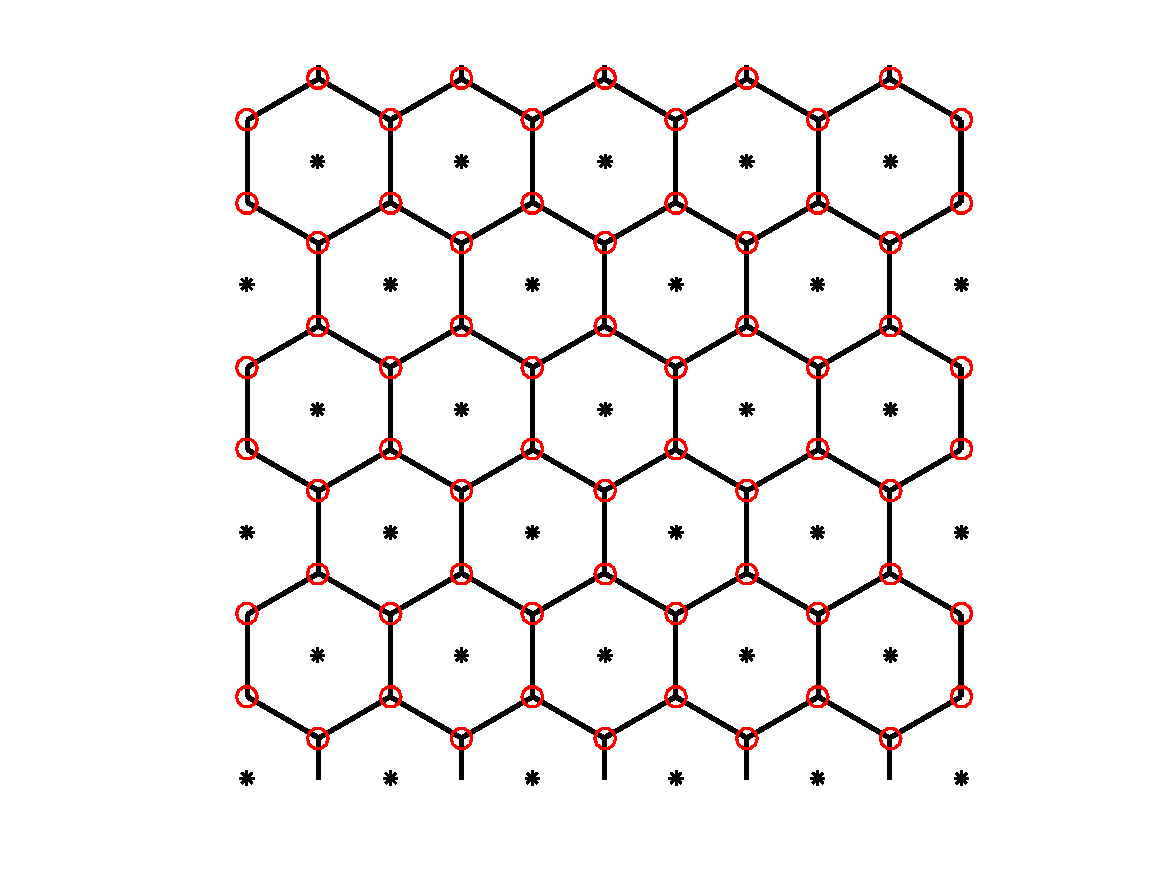
\includegraphics[width=7cm]{HexagTiling.pdf} \hspace{0.5cm}
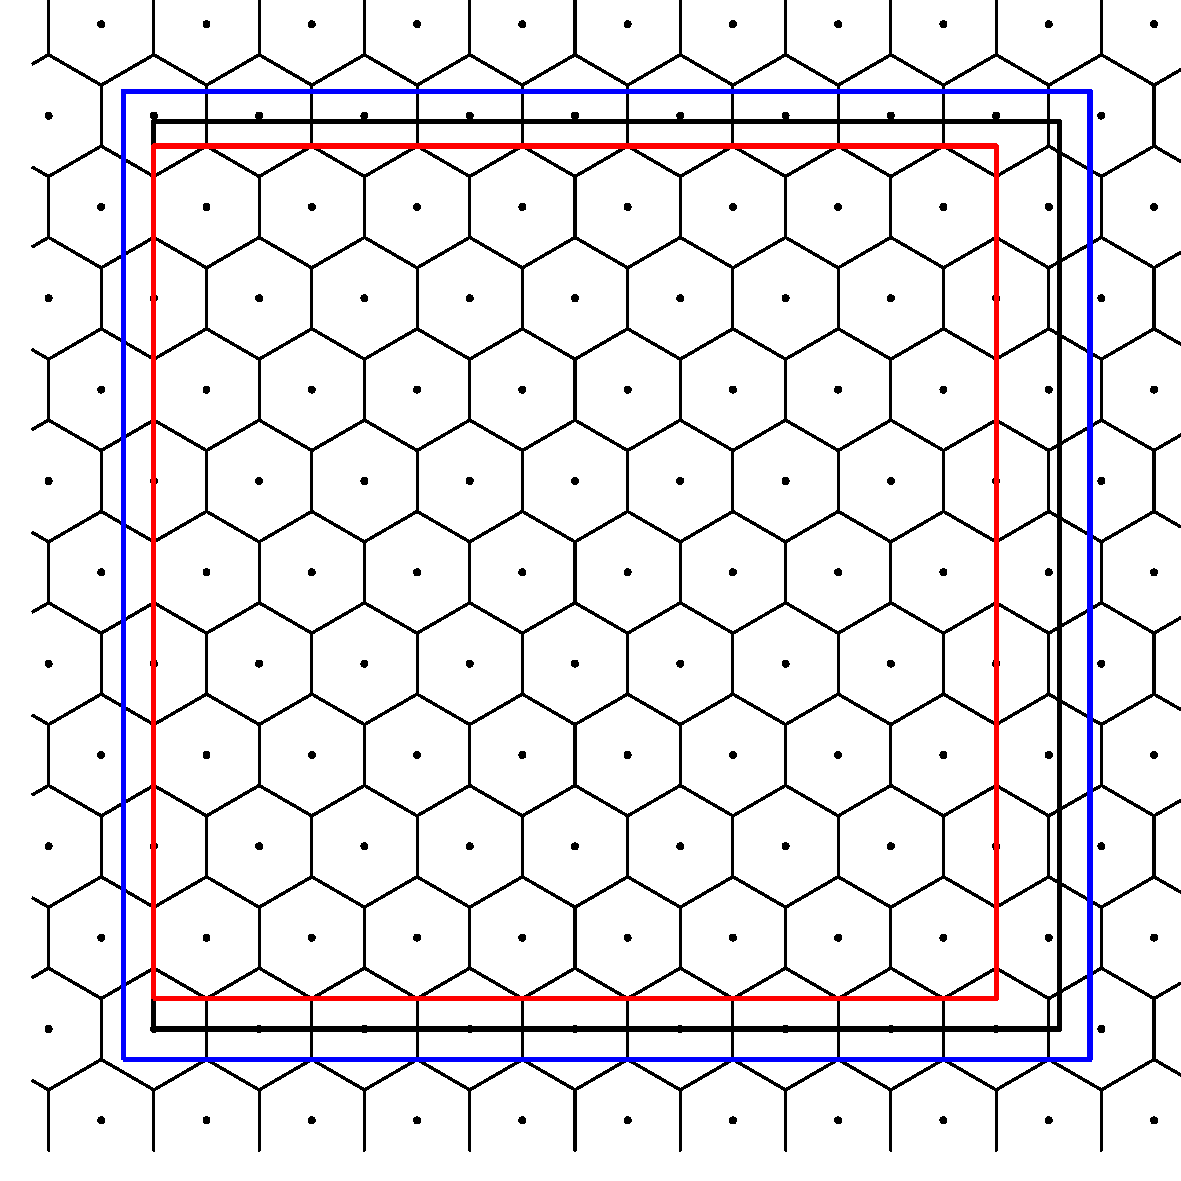
\includegraphics[width=5cm]{UUepsVHexag.pdf}
\end{center}
\caption{On the left: Hexagonal tiling restricted to a square domain $(0,T)^2$. On the right: the domains $U$ (black square), $U_\eps$ (red rectangle) and $U^{\eps}$ (blue square).}\label{HexagTiling:fig}
\end{figure}

We first introduce some notations for the tiling with hexagons. For $\theta\in\R$, we will denote by $e_\theta$ the unit vector of coordinates $(\cos\theta,\sin\theta)$. Let $\eps>0$ and let us consider a regular tiling with hexagons of ``size'' $\eps$ where the set of the centers of the hexagons is given by
\[
\calC_\eps = \left\{ k_1 \sqrt{3}\eps e_0 + k_2 \sqrt{3}\eps e_{\pi/3} \, ; \, k_1, k_2 \in \Z \right\} =
\left\{ \eps \left(\left(k_1+\frac{1}{2}k_2\right) \sqrt{3}, \frac{{3}}{2} k_2\right)\, ; \, k_1, k_2 \in \Z \right\}
\]
The distance between the centers of two neighbouring hexagons is $\sqrt{3}\eps$, the side length of the hexagons is $\eps$ and the area of each hexagon is $ \tfrac{3\sqrt{3}}{2}\eps^2$. The vertices of the hexagons are the set of points $\calV_\eps$ given by
\[
\calV_\eps = \calC_\eps + \left\{ \eps e_{\frac{\pi}{6} + n
\frac{\pi}{3}} \, ; \, 0\leq n \leq 5 \right\}.
\]
On Figure~\ref{HexagTiling:fig}, we show such a tiling with regular hexagons. The points of $\calC_\eps$ are plotted with black stars and the points of $\calV_\eps$ are the vertices of the hexagons marked by small red circles. For $z\in \calC_\eps$ we will denote by $\calD(z,\eps)$ the (open) hexagon of center $z$ and size $\eps$. Notice that the distance between a vertex $v\in\calV_\eps$ and the centers of its three neighbouring hexagons is equal to $\eps$, that is also the side length of the hexagons.

Finally we will denote by $\calE_\eps$ the set of edges. Each edge is a segment of length $\eps$ between two neighbouring vertices of $\calV_\eps$ and we will sometimes identify an edge $w\in\calE_\eps$ with its middle point. The set of edges is the union of three sets, depending on the orientation of the edge, and that are denoted by $\calE_\eps^{\pi/2}$, $\calE_\eps^{\pi/6}$ and $\calE_\eps^{-\pi/6}$. In order to remove boundary effects, when considering a square domain $U=(0,T)^2$, we will consider the enlarged domain $U^{\eps}=(-\tfrac{\eps}{2},T+\tfrac{\eps}{2})\times (-\tfrac{\eps}{2},T+\tfrac{\eps}{2})$ as well as the restricted domain
\[
U_\eps=\left(0,\sqrt{3}\eps
\left\lfloor \frac{T}{\sqrt{3}\eps}\right\rfloor\right)\times
\left(\frac{\eps}{2},3\eps\left\lfloor\frac{T+\eps/2}{{3}\eps}\right\rfloor-\frac{\eps}{2}\right)
\]
such that
\[
U_\eps\subset U\subset U^{\eps}.
\]
This will ensure that no
edge (seen as an open segment) of the tiling in $U_\eps$ intersects $\partial U_\eps$, and that each midpoint $w\in \calE_\eps \cap U_\eps$ is the middle of two centers in ${\calC}_\eps\cap U^{\eps}$ (see Figure~\ref{HexagTiling:fig} right).

To give some order of magnitudes, notice that the cardinality of the different sets of points are
\[
\left|\calC_\eps \cap U \right|\simeq \frac{2}{3\sqrt{3}} \frac{T^2}{\eps^2}, \quad
\left|\calE_\eps \cap U \right|\simeq \frac{2}{\sqrt{3}} \frac{T^2}{\eps^2}
\quad \text{ and } \quad \left|\calV_\eps \cap U \right|\simeq \frac{4}{3\sqrt{3}} \frac{T^2}{\eps^2}.
\]
These equivalents also hold when we consider $U_\eps$ or $U^\eps$ in place of $U$.


We denote by $\PC^{\Hex}_\eps(U^{\eps})$ the set of piecewise constant functions on the hexagonal tiling in $U^{\eps}$. A function $f\in
\PC^{\Hex}_\eps(U^{\eps})$ can be identified with the finite set of values $\{ f(y)\}_{y\,\in\,\calC_\eps\, \cap\,U^{\eps}}$. To have a function that is defined everywhere, we adopt the convention that the value of $f$ on an edge is equal to the mean value of its two neighbouring centers, and the value at a vertex is the mean value of its three neighbouring centers. For $f\in \PC^{\Hex}_\eps(U^{\eps})$, we denote for each vertex $v\in {\calV}_\varepsilon$, the three ordered neighbouring values at $v$ by $f^{(1)}(v)\le f^{(2)}(v)\le f^{(3)}(v)$. And for each $w\in\calE_\eps$, we denote by $f^+(w)$ and $f^-(w)$, respectively the maximum and the minimum of the two values of $f$ on the two sides of $w$.


\begin{prop}\label{level-int-discr:prop}
Let $f\in\PC^{\Hex}_\eps(U^{\eps})$. The function $f$ has a finite total variation in $U_\eps$ and for $h\in C_b(\R)$ and $H$ a primitive of $h$, the level perimeter integral of $f$ satisfies
\[
\LP_f\left(h,U_\eps\right)= \eps \sum_{w\,\in\,\calE_\eps\,\cap\,U_\eps} \left[H\left(f^+(w)\right) - H\left(f^-(w)\right)\right].
\]

Moreover, the function $f$ is of finite level total curvature integral and the level total curvature integral of $f$ satisfies
\[
\LTC_{f}(h,U_\eps)=\frac{\pi}{3}
\sum_{v\,\in\,\calV_\varepsilon\,\cap\,U_\eps} \left[H\left(f^{(3)}(v)\right) + H\left(f^{(1)}(v)\right)-2H\left(f^{(2)}(v)\right)\right].
\]

In particular,
\begin{align*}
\LP_f(U_\eps)&=\eps \sum_{w\,\in\,\calE_\eps\,\cap\,U_\eps} \left[f^+(w) -
f^-(w)\right]
\\
\intertext{and}
\LTC_{f}(U_\eps)&=\frac{\pi}{3}
\sum_{v\,\in\,{\calV}_\varepsilon\,\cap\,U_\eps} \left[f^{(3)}(v) +
f^{(1)}(v)-2f^{(2)}(v)\right].
\end{align*}
\end{prop}


\begin{proof}
Let us start with the level perimeter integral. Since $f\in\PC^{\Hex}_\eps(U^{\eps})$, for any $t\in\R$, the excursion set $E_f(t)\cap U_\eps$ is a union of hexagons (or parts of hexagons on the boundary), and an edge $w\in\calE_\eps$ is part of the boundary of $E_f(t)$ in $U_\eps$ if and only if $f^-(w) < t \leq f^+(w)$. We also recall that all edges in $\calE_\eps$ have the same length, that is equal to $\eps$ and that an edge in $U_\eps$ is entirely contained in $U_\eps$. Moreover, since $U_\eps$ is bounded, $t\mapsto \Per (E_f(t),U_\eps)$ is piecewise constant with compact support and therefore we have, for $h \in C_b(\R)$, denoting $H$ a primitive of $h$,
\begin{align*}
\LP_f(h,U_\eps) & = \int_\R h(t) \Per \left(E_f(t),U_\eps\right) \, dt = \int_\R h(t)
\left(\sum_{w\,\in\,\calE_\eps\,\cap\,U_\eps} \eps\ind_{f^-(w)\,<\,t\,\leq\,f^+(w)} \right) \, dt \\
& = \eps \sum_{w\,\in\,\calE_\eps\,\cap\,U_\eps} \int_{f^-(w)}^{f^+(w)} h(t) \;\, dt =
\eps \sum_{w\,\in\,\calE_\eps\,\cap\,U_\eps} \left[H\left(f^+(w)\right) - H\left(f^-(w)\right)\right].
\end{align*}

\begin{figure}[h]
\centerline{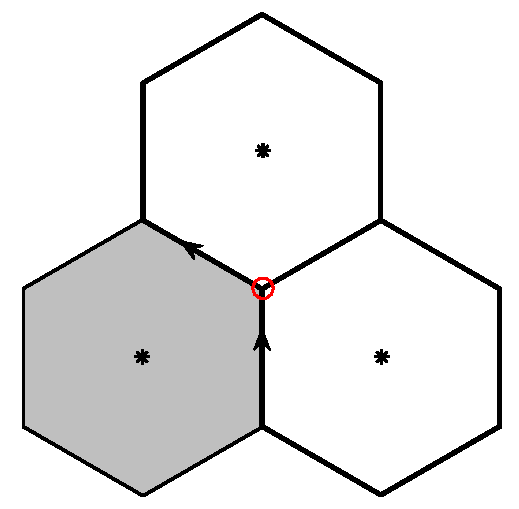
\includegraphics[width=4cm]{TurningAngleHexag1.pdf}
\hspace{2cm}
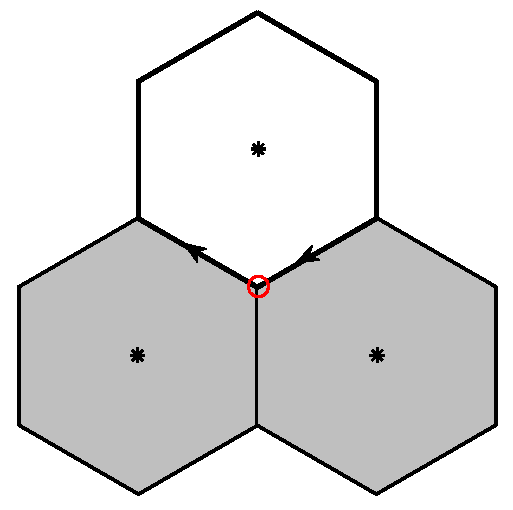
\includegraphics[width=4cm]{TurningAngleHexag2.pdf} }
\caption{The turning angle at a vertex $v$ is else $+\frac{\pi}{3}$ if $f^{(2)}(v)<t\leq f^{(3)}(v)$ (since in that case the set $\{f\geq t\}$ is made of one hexagon, see left figure) or $-\frac{\pi}{3}$ if $f^{(1)}(v)<t\leq f^{(2)}(v)$ (since in that case the set $\{f\geq t\}$ is made of two hexagons, see right figure).}\label{LTCHexagTiling:fig}
\end{figure}

For the level total curvature integral the computations are similar. The boundary of an excursion set $E_f(t)$ in $U_\eps$ is a curve that is piecewise linear since it is made of edges in $\calE_\eps$. Its curvature at regular points is then $0$, and it has only corner points at vertices $v\in\calV_\eps$, where the turning angle is else $\frac{\pi}{3}$ if $f^{(2)}(v)<t\leq f^{(3)}(v)$ or $-\frac{\pi}{3}$ if $f^{(1)}(v)<t\leq f^{(2)}(v)$ (see Figure~\ref{LTCHexagTiling:fig}). Therefore

\begin{align*}
\LTC_f\left(h,U_\eps\right) & = \int_\R h(t) \TC \left(\partial E_f(t) \cap U_\eps\right) \, dt \\
&= \int_\R h(t)
\left(\sum_{v\,\in\,\calV_\eps\,\cap\,U_\eps} \frac{\pi}{3}\left(
\ind_{f^{(2)}(v)\,<\,t\,\leq\,f^{(3)}(v)} - \ind_{f^{(1)}(v)\,<\,t\,\leq\,f^{(2)}(v)} \right) \right) \, dt \\
& = \frac{\pi}{3} \sum_{v\,\in\,\calV_\eps\,\cap\,U_\eps}
\int_{f^{(2)}(v)}^{f^{(3)}(v)} h(t) \, dt -\int_{f^{(1)}(v)}^{f^{(2)}(v)} h(t) \, dt \\
x^{2} & =
\frac{\pi}{3} \sum_{v\,\in\,\calV_\varepsilon\,\cap \,U_\eps} \left[H\left(f^{(3)}(v)\right) + H\left(f^{(1)}(v)\right)-2H\left(f^{(2)}(v)\right)\right].\qedhere
\end{align*}
\end{proof}


\subsection{The square tiling case}\label{LPLTCSq:subsec}

\begin{figure}[h]
\begin{center}
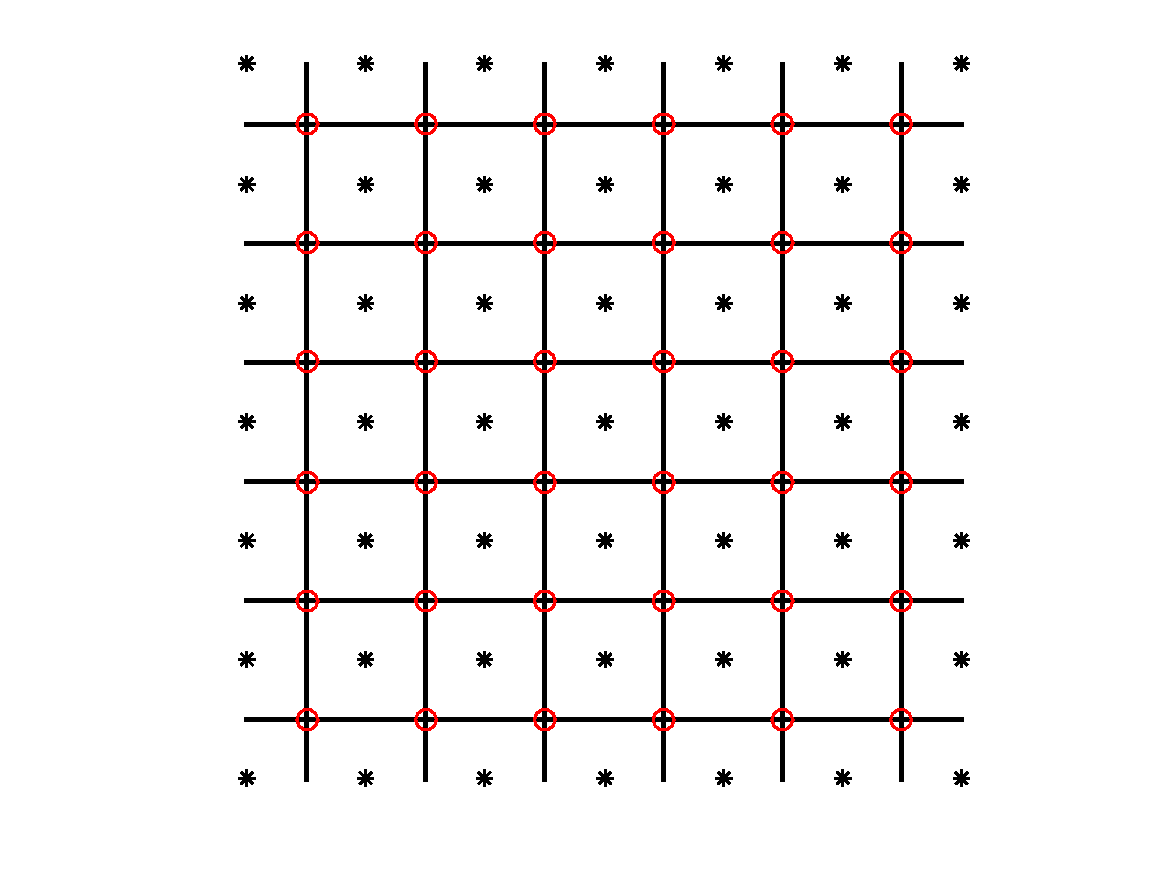
\includegraphics[width=7cm]{FigSquareTiling.pdf}
\hspace{0.5cm}
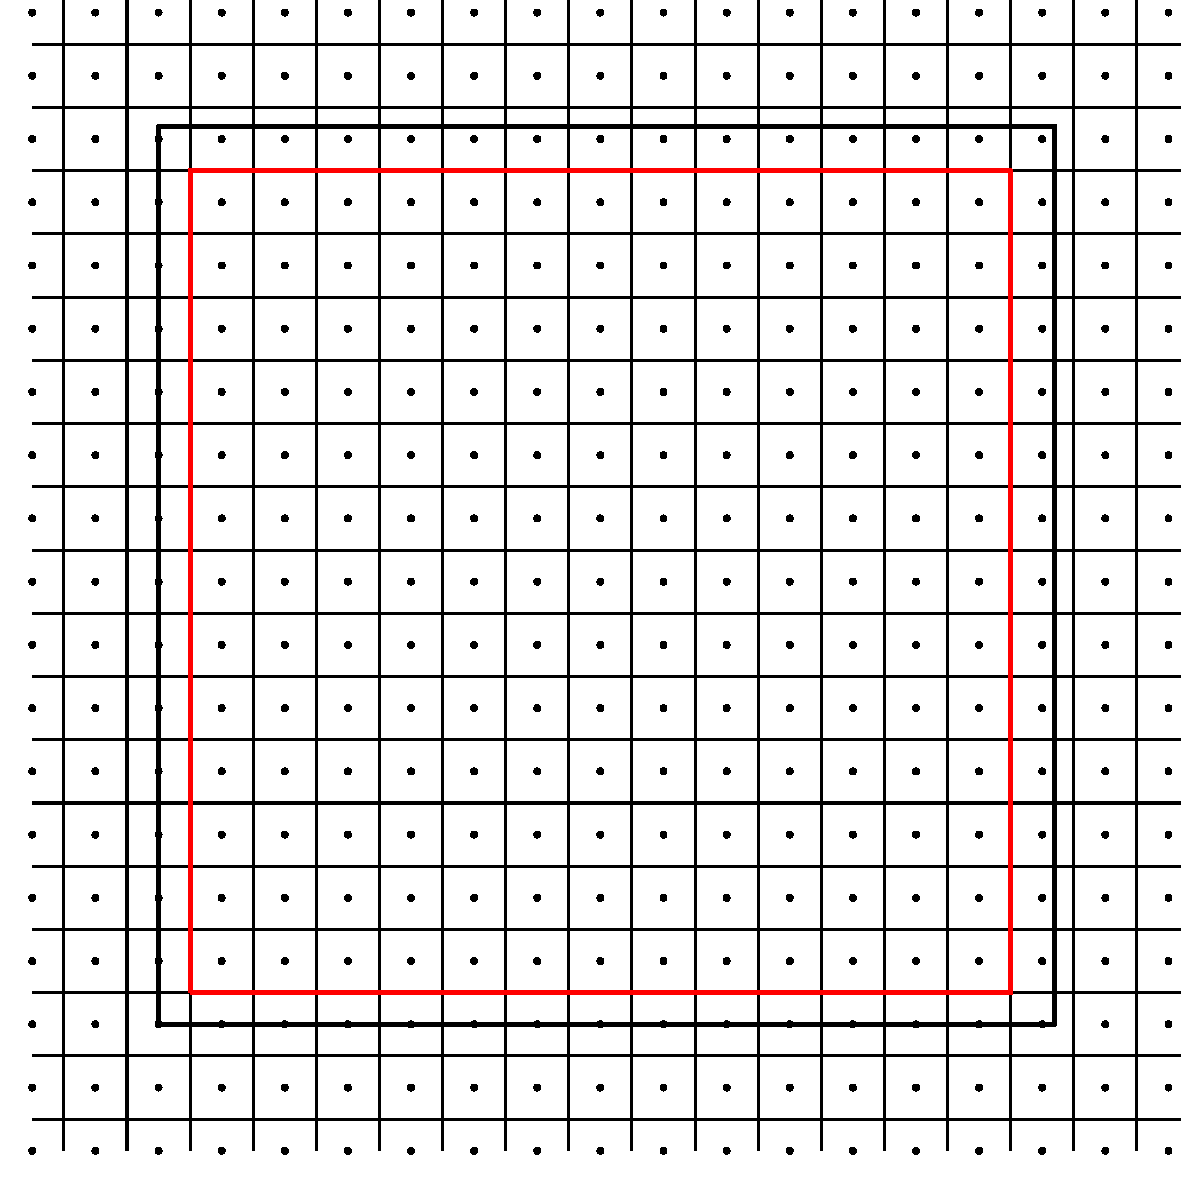
\includegraphics[width=5cm]{UUepsVSquare.pdf}
\end{center}
\caption{On the left: a tiling with squares restricted to a square domain $(0,T)^2$. The centers (set $\calC_\eps$) of the squares are the black stars, and the vertices (set $\calV_\eps$) are the points marked by a red circle. On the right: the domain $U$ (black square) and $U_\eps$ (red square).}\label{SquareTiling:fig}
\end{figure}

We now consider the case of a tiling with squares. This is the case used in practice for digital images since they are defined on (square) pixels (contraction of \emph{picture elements}). Let $\eps>0$ and let us consider a regular tiling with squares of ``size'' (side length) $\eps$ where the set of the centers of the squares is given by
\[
\calC_\eps = \left\{ k_1 \eps e_0 + k_2 \eps e_{\pi/2} \, ; \, k_1, k_2
\in \Z \right\} = \left\{ \eps (k_1,k_2) \, ; \, k_1, k_2 \in \Z \right\}.
\]
The side length of the squares is $\eps$ and the area of each square is $\eps^2$. The vertices of the squares are the set of points $\calV_\eps$ given by
\begin{align*}
\calV_\eps &= \calC_\eps + \left\{ \frac{\sqrt{2}}{2}\eps e_{\frac{\pi}{4} + n
\frac{\pi}{2}} \, ; \, 0\leq n \leq 3 \right\} \\
&= \left\{ \left(k_1 +\frac{1}{2}\right)
\eps e_0 + \left(k_2 +\frac{1}{2}\right) \eps e_{\pi/2} \, ; \, k_1, k_2 \in \Z \right\}.
\end{align*}
We will denote by $\calE_\eps$ the set of edges. Each $w\in\calE_\eps$ is a segment of length $\eps$ that is else horizontal or vertical. For $z\in
\calC_\eps$ we will denote by $\calD(z,\eps)$ the (open) square of center $z$ and size $\eps$. Finally, notice that the distance between a vertex $v\in\calV_\eps$ and the centers of its four neighbouring squares is equal to $\eps\sqrt{2}/2$.



When considering a square domain $U=(0,T)^2$ and $\eps>0$, we will define here the restricted domain $U_\eps=(0,\eps \lfloor
\tfrac{T}{\eps}\rfloor)^2$. For the enlarged domain $U^\eps$, since we already have that each midpoint $w\in \calE_\eps \cap U_\eps$ is the middle of two centers in ${\calC}_\eps\cap U$ (see Figure~\ref{SquareTiling:fig} right), we can simply set $U^\eps=U$.

Let us notice that here we have
\[
\left|\calC_\eps\cap U\right|\simeq \frac{T^2}{\eps^2} ; \quad\left|\calE_\eps\cap U\right|\simeq 2 \frac{T^2}{\eps^2}
\quad \text{ and } \quad \left|\calV_\eps\cap U\right|\simeq \frac{T^2}{\eps^2}.
\]
The same approximations hold when $U$ is replaced by $U_\eps$.

%\bigskip

When dealing with a tiling with squares, the definition of connectivity is not unique. Indeed we can say that two squares are neighbours if they have a common edge (this is the $4$-connectivity), or only as soon as they have a common corner (this is the $8$-connectivity). Now, in fact, these two connectivities are ``complementary''. Indeed, if we want a discrete version of the Jordan curve theorem to hold, we have to state it in the following way (\cite{Rosenfeld79}) : the complement of a 4-connected simple closed discrete curve (sequence of squares) is made of exactly two 8-connected components.


%\bigskip

We will denote by $\PC^{\Sq}_\eps(U)$ the set of functions $f$ defined on $U$ that are piecewise constant on the tiling with regular squares of size $\eps>0$. Such a function can be simply identified to the finite set of values $\{f(z) \}_{z\,\in\,\calC_\eps\,\cap\,U}$. The value of $f$ along an edge is taken as being the mean value of its two neighbouring centers, while its value at a vertex is given by the mean value of its four neighbouring centers. Since we have to consider two different total curvatures according to the choice of connectivity, we write $\TC^4(\partial E_f(t) \cap U_\eps)$ and $\TC^8(\partial E_f(t)\cap U_\eps)$ such that, for $h$ a bounded continuous function,
\begin{equation}\label{TCsquare}
\LTC^\dd_f(h,U)=\int_{\R}h(t) \TC^\dd\left(\partial E_f(t)\cap U\right) dt,\,\text{ for } \dd\in\{4,8\}.
\end{equation}

We denote for each vertex $v\in {\calV}_\varepsilon$, the four ordered neighbouring values at $v$ by $f^{(1)}(v)\le f^{(2)}(v)\le f^{(3)}(v) \le f^{(4)}(v)$. And for each $w\in\calE_\eps$, we denote by $f^+(w)$ and $f^-(w)$, respectively the maximum and the minimum of the two values of $f$ on the two sides of $w$.


\begin{prop}\label{level-int-discr-square:prop}
Let $f\in\PC^{\Sq}_\eps(U)$. The function $f$ has a finite total variation in $U_\eps$ and for $h \in C_b(\R)$ and $H$ a primitive of $h$, the level perimeter integral of $f$ satisfies
\[
\LP_f(h,U_\eps)= \eps \sum_{w\,\in\,\calE_\eps\,\cap \,U_\eps} \left[H\left(f^+(w)\right) - H\left(f^-(w)\right)\right].
\]

Moreover, the function $f$ is of finite level total curvature integral and the level total curvature integrals of $f$ satisfy
\begin{align*}
\LTC^4_{f}(h,U_\eps) & = \frac{\pi}{2} \sum_{v\,\in\, \calV_\varepsilon\,\cap\,U_\eps} \left[H\left(f^{(1)}(v)\right) + H\left(f^{(4)}(v)\right)- H\left(f^{(3)}(v)\right) - H\left(f^{(2)}(v)\right)\right] \\
&\quad+ \pi \sum_{v\,\in\,\calV_\eps\,\cap\,U_\eps} \left[H\left(f^{(3)}(v)\right) - H\left(f^{(2)}(v)\right)\right]\ind_{c(v)\,=\,\cross},
\end{align*}
and
\begin{align*}
\LTC^8_{f}(h,U_\eps) & = \frac{\pi}{2} \sum_{v\,\in\, \calV_\varepsilon\,\cap\,U_\eps} \left[H\left(f^{(1)}(v)\right) + H\left(f^{(4)}(v)\right)- H\left(f^{(3)}(v)\right) - H\left(f^{(2)}(v)\right)\right] \\
&\quad - \pi
\sum_{v\,\in\,\calV_\eps\,\cap\,U_\eps} \left[H\left(f^{(3)}(v)\right) - H\left(f^{(2)}(v)\right)\right]
\ind_{c(v)\,=\,\cross},
\end{align*}
where $c(v)=\cross$ denotes the event that the configuration at $v$ is ``a cross '' (meaning that $f^{(1)}$ and $f^{(2)}$ are achieved at two ``opposite'' squares (see Figure~\ref{LTCCross:fig})).
\end{prop}

\begin{proof}
Let us start with the level perimeter integral. Since $f\in\PC^{\Sq}_\eps(U)$, for any $t\in\R$, the excursion set $E_f(t)\cap U_\eps$ is a union of squares, and an edge $w\in\calE_\eps$ is part of the boundary of $E_f(t)$ in $U_\eps$ if and only if $f^-(w) < t \leq f^+(w)$. We also recall that all edges in $\calE_\eps$ have the same length, that is equal to $\eps$. Since $t\mapsto \Per (E_f(t;U_\eps))$ is piecewise constant with compact support, we have, for $h\in C_b(\R)$ and $H$ a primitive of $h$,
\begin{align*}
\LP_f(h,U_\eps) & = \int_\R h(t) \Per \left(E_f(t),U_\eps\right) \, dt = \int_\R h(t)
\left(\sum_{w\,\in\,\calE_\eps\,\cap\,U} \eps\ind_{f^-(w)\,<\,t\,\leq\,f^+(w)} \right) \, dt \\
& = \eps \sum_{w\,\in\,\calE_\eps\,\cap\,U_\eps} \int_{f^-(w)}^{f^+(w)} h(t) \:\, dt =
\eps \sum_{w\,\in\,\calE_\eps\,\cap\,U_\eps} \left[H\left(f^+(w)\right) - H\left(f^-(w)\right)\right].
\end{align*}

\begin{figure}[!htbp]
\centerline{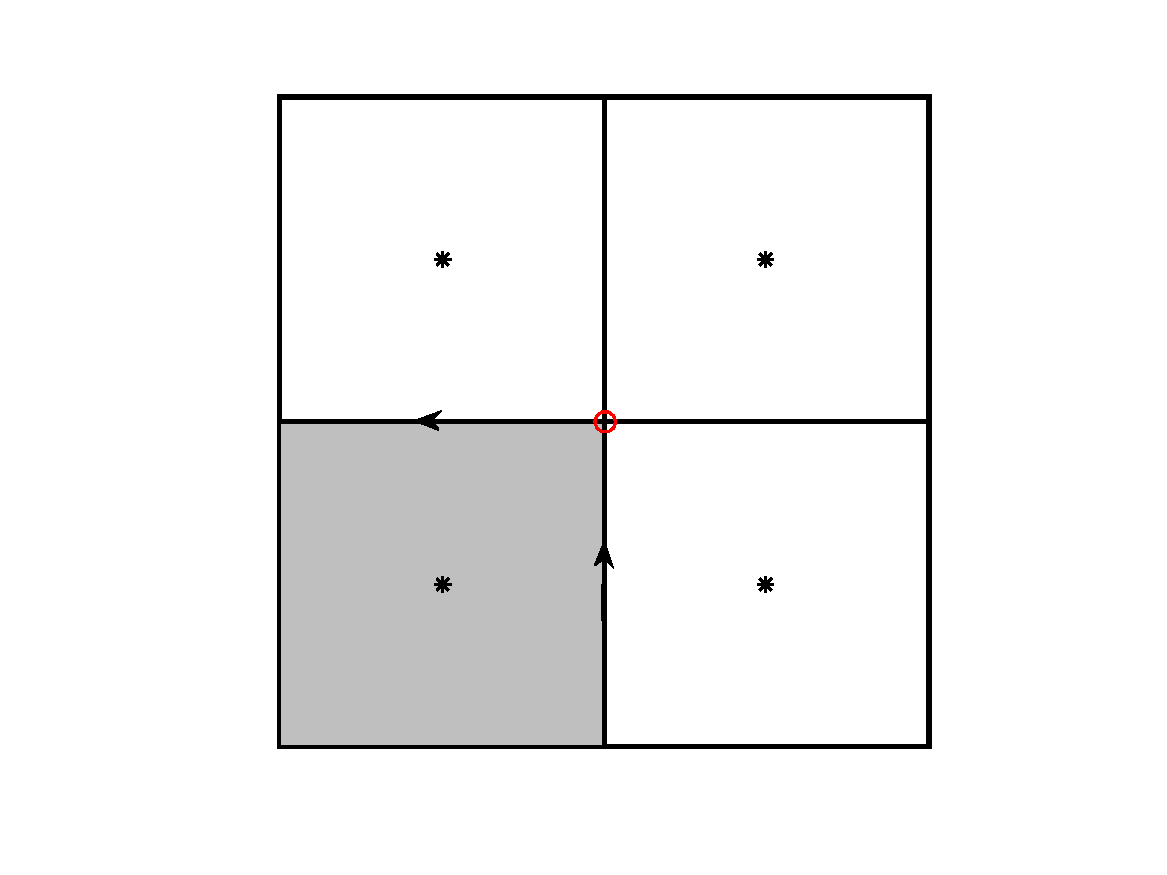
\includegraphics[width=5cm]{TurningAngleSquares1.pdf}
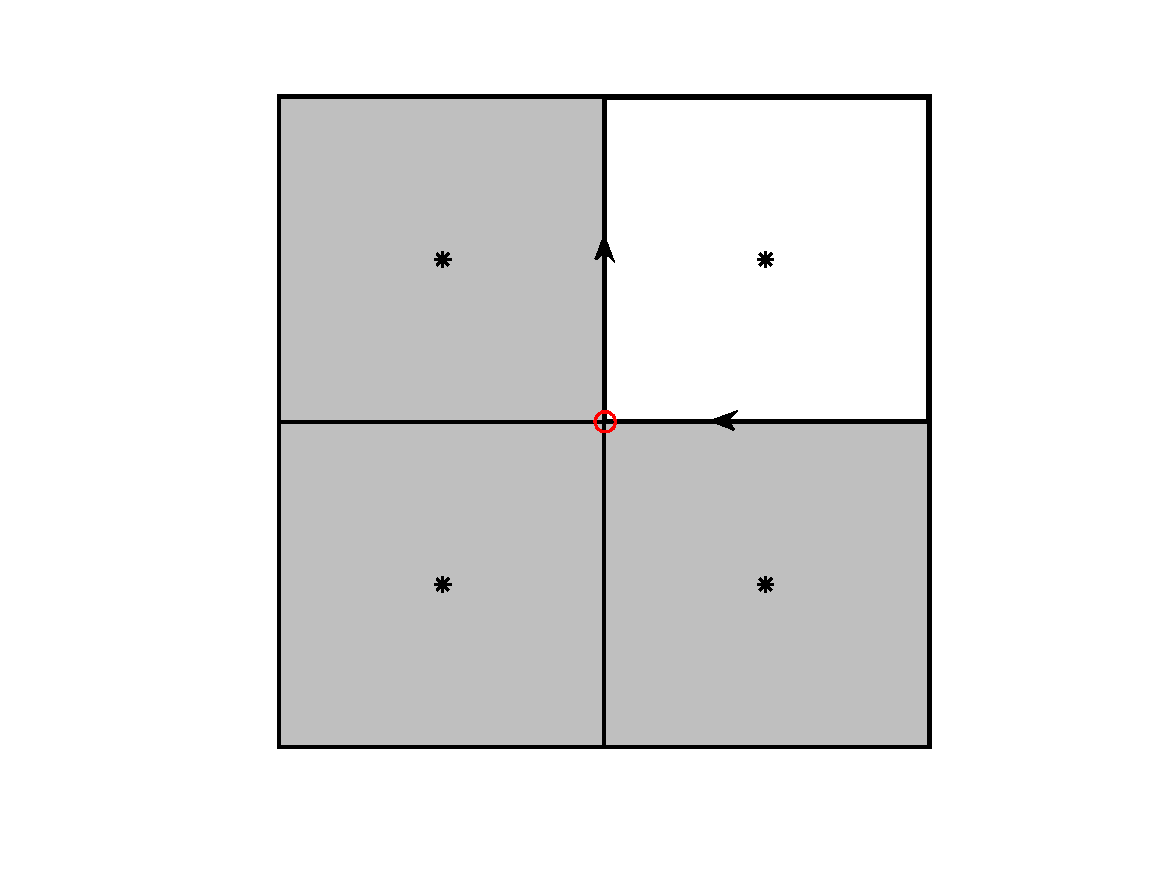
\includegraphics[width=5cm]{TurningAngleSquares3.pdf}
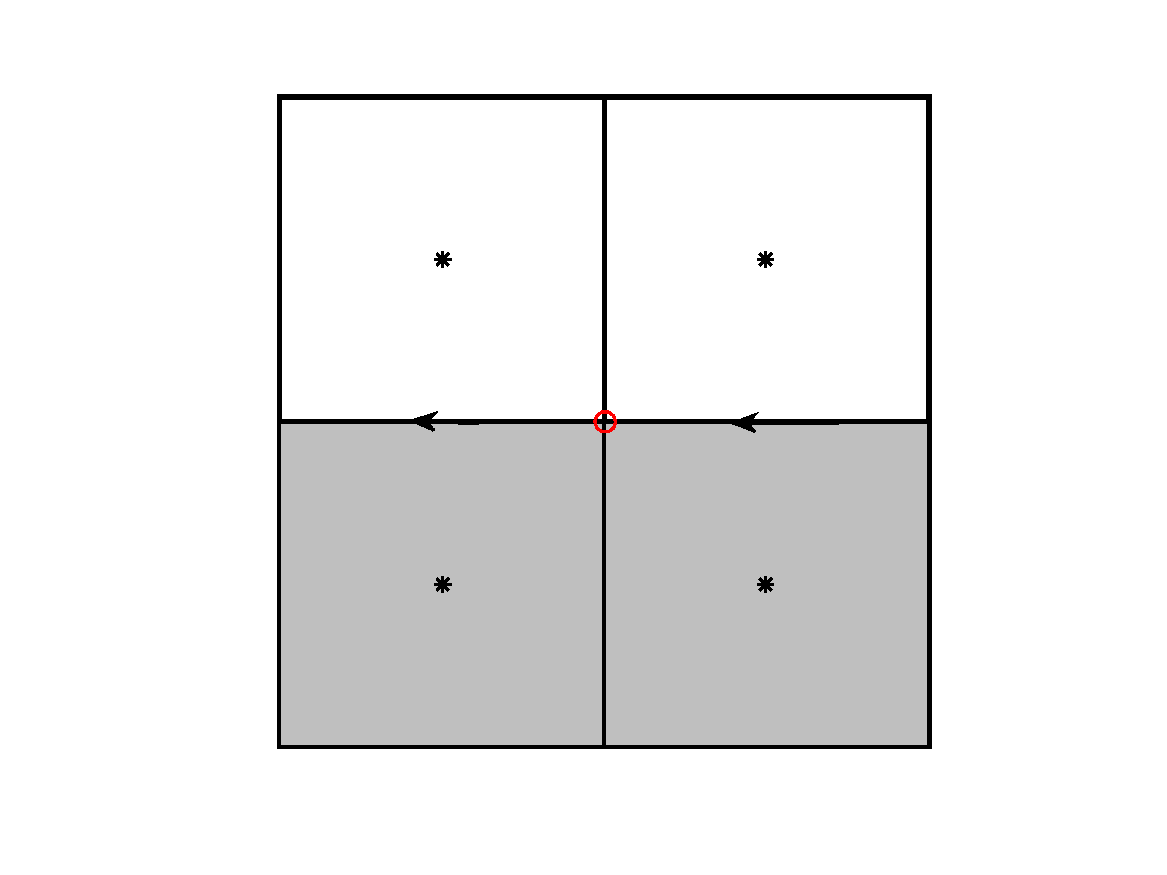
\includegraphics[width=5cm]{TurningAngleSquares2.pdf} }
\caption{The turning angle at a vertex $v$ is else $+\tfrac{\pi}{2}$ if $f^{(3)}(v)<t\leq f^{(4)}(v)$ (since in that case the set $\{f\geq t\}$ is made of one square, see the left-most figure), or $-\tfrac{\pi}{2}$ if $f^{(1)}(v)<t\leq f^{(2)}(v)$ (since in that case the set $\{f\geq t\}$ is made of three squares, see the middle figure), or $0$ if $f^{(2)}(v)<t\leq f^{(3)}(v)$ and the configuration at $v$ is not a cross (since in that case the set $\{f\geq t\}$ is made of two adjacent squares, see the right-most figure).}\label{LTCSquareTiling:fig}
\end{figure}

\begin{figure}[!htbp]
\centerline{
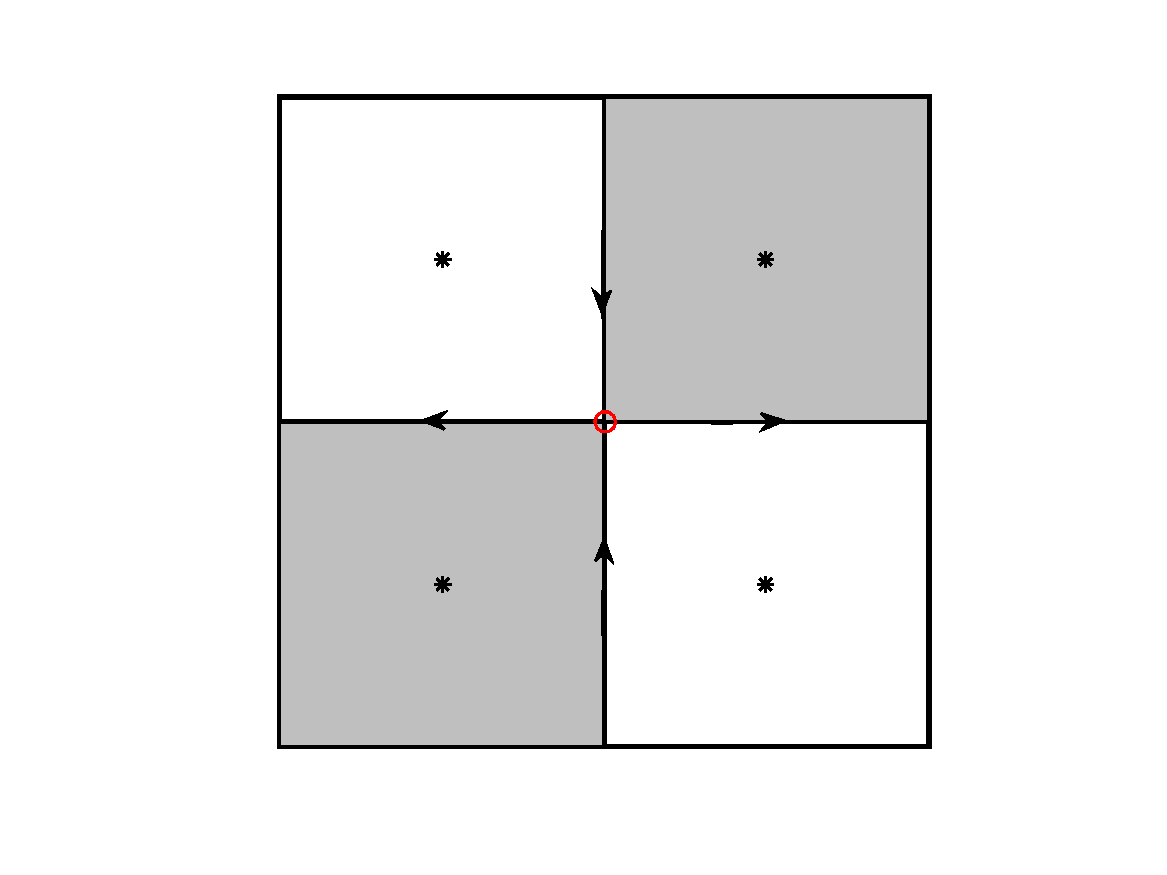
\includegraphics[width=5.5cm]{TurningAngleSquaresX.pdf}
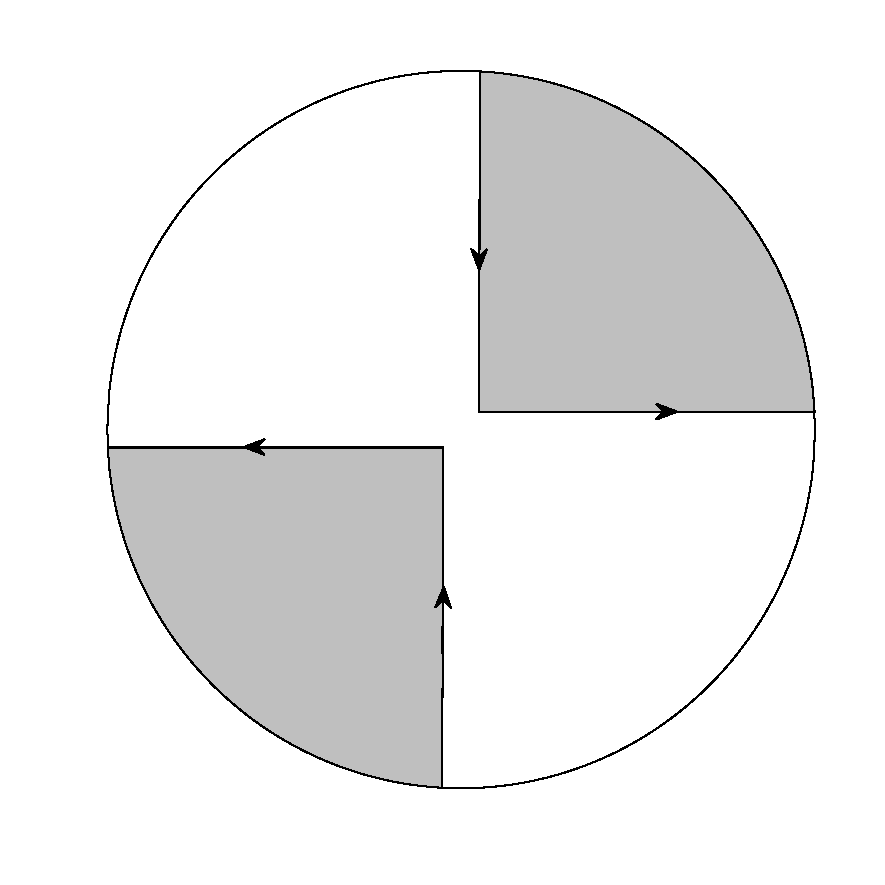
\includegraphics[width=4cm]{TurningCross4cc.pdf}
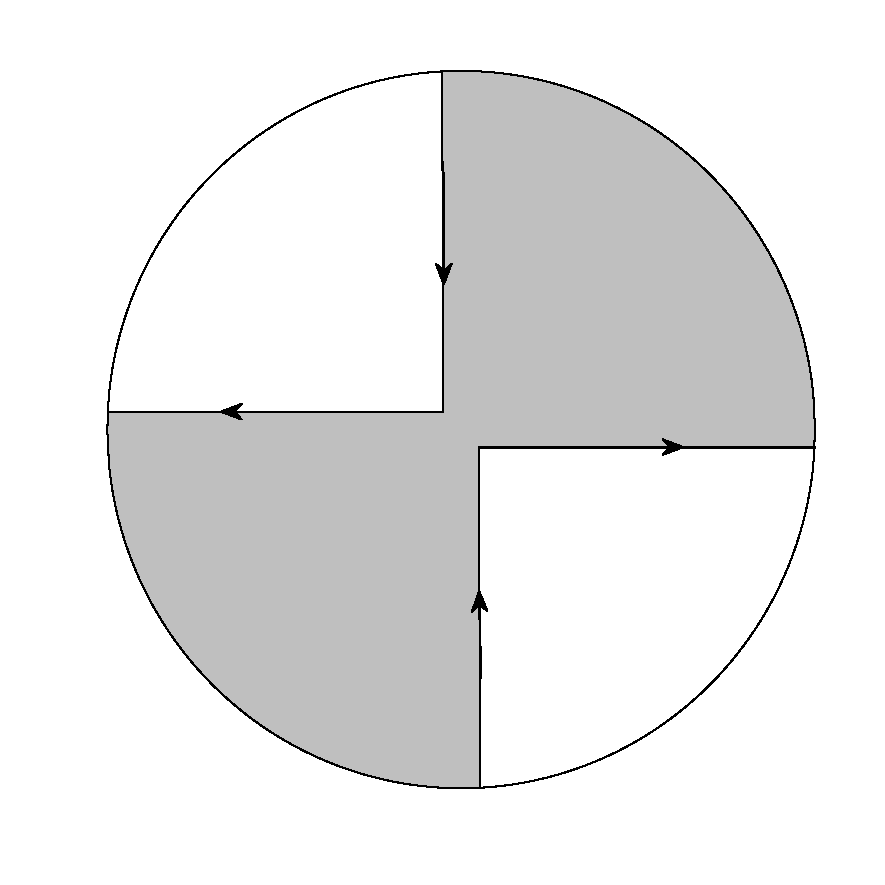
\includegraphics[width=4cm]{TurningCross8cc.pdf} }
\caption{ If $f^{(2)}(v)<t\leq f^{(3)}(v)$ and the configuration at $v$ is a cross (left figure), the turning angle at a vertex $v$ is $\pi=\pi/2 +\pi/2$ (in $4-$connectivity, since it is equivalent to the ``zoom'' presented in the middle figure) or $-\pi=-\pi/2 -\pi/2$ (in $8-$connectivity, see the ``zoom'' on the right figure).}\label{LTCCross:fig}
\end{figure}

For the level total curvature integral the computations are also similar to the ones in the case of hexagons. However, we have to consider the two different types of connectivity. The boundary of an excursion set $E_f(t)$ in $U_\eps$ is a curve that is piecewise linear since it is made of edges in $\calE_\eps$. Its curvature at regular points is then $0$, and it has only corner points at vertices $v\in\calV_\eps$, where the turning angle $\beta$ is (see Figure~\ref{LTCSquareTiling:fig}):
\begin{itemize}
\item $\beta=\frac{\pi}{2}$ if $f^{(3)}(v)<t\leq f^{(4)}(v)$ ;
\item $\beta= - \frac{\pi}{2}$ if $f^{(1)}(v)<t\leq f^{(2)}(v)$ ;
\item If $f^{(2)}(v)<t\leq f^{(3)}(v)$, then $\beta=0$ if the configuration at $v$ is not a ``cross'' (see Figure~\ref{LTCSquareTiling:fig}), whereas if the configuration at $v$ is a cross (see Figure~\ref{LTCCross:fig}), then $\beta=\pi$ in $4-$connectivity and $\beta=-\pi$ in $8-$connectivity.
\end{itemize}



Therefore,
\begin{multline*}
\LTC^4_f(h,U_\eps)\\
\begin{aligned}
& = \frac{\pi}{2} \sum_{v\,\in\,\calV_\eps\,\cap\,U_\eps}
\int_{f^{(3)}(v)}^{f^{(4)}(v)} h(t) \, dt -\int_{f^{(1)}(v)}^{f^{(2)}(v)} h(t) \, dt + \pi
\sum_{v\,\in\,\calV_\eps\,\cap\,U_\eps} \ind_{c(v)\,=\,\cross}
\int_{f^{(2)}(v)}^{f^{(3)}(v)} h(t) \, dt \\
& =
\frac{\pi}{2} \sum_{v\,\in\,\calV_\varepsilon\,\cap\,U_\eps} \left[H\left(f^{(1)}(v)\right) + H\left(f^{(4)}(v)\right)- H\left(f^{(3)}(v)\right) - H\left(f^{(2)}(v)\right)\right] \\
& + \pi
\sum_{v\,\in\,\calV_\eps\,\cap\,U} \left[H\left(f^{(3)}(v)\right) - H\left(f^{(2)}(v)\right)\right]
\ind_{c(v)\,=\,\cross}.
\end{aligned}
\end{multline*}
For $\LTC^8_f(h,U_\eps)$ the computation is the same, except that the $+\pi$ in front of the second sum is changed into $-\pi$.
\end{proof}

A convenient way to get rid of the connectivity ambiguity is to consider a kind of ``6-connectivity'' by setting
\[
\LTC^6_f(h,U_\eps) := \frac{1}{2} \left(\LTC^4_f(h,U_\eps) +\LTC^8_f(h,U_\eps) \right).
\]
Then, the ``cross'' configuration doesn't appear anymore in the formula, since, using the above results, we simply have
\[
\LTC^6_f(h,U_\eps) = \frac{\pi}{2} \sum_{v\,\in\,\calV_\varepsilon\,\cap\,U_\eps} \left[H\left(f^{(1)}(v)\right) +
H\left(f^{(4)}(v)\right)- H\left(f^{(3)}(v)\right) - H\left(f^{(2)}(v)\right)\right].
\]



\begin{rema}
Let us note that these formulas are of course linked with numerical computations of discrete topology. Actually, when considering a set $E\subset U$ we can choose $f\in \PC^{\Sq}_\eps(U)$ corresponding to its discretization of size $\eps$ by taking $f(z)=1$ when $z \in \calC_\eps\cap E$ and $f(z)=0$ otherwise. Now, since the values $\{f(z) \}_{z\,\in\,\calC_\eps\,\cap\,U}$ are in $\{0,1\}$ and those of $f$ in $\{0,1/4,1/2,3/4,1\}$, one can take $h\in C_b(\R)$ a non-negative function with support in $(3/4,1)$ such that $\int_{\R}h=\int_{3/4}^1h=1$. On the one hand, we clearly have
\begin{align*}
\LTC^{\dd}_f(h,U_\eps)&=\int_{3/4}^1\TC^{\dd}\left(\partial E_{f}(t)\cap U_\eps\right)h(t)dt\\
&=\TC^{\dd}\left(\partial E_{f}(1)\cap U_\eps\right)\int_{3/4}^1h(t)dt=\TC^{\dd}\left(\partial E_{f}(1) \cap U_\eps\right).
\end{align*}
\end{rema}
On the other hand, choosing $H(t)=\int_{-\infty}^th(t)$, since $f^{(j)}(v) \in \{0,1\}$ for $1\le j\le 4$, one has $H(f^{(j)}(v))=f^{(j)}(v)$ and
\begin{align*}
\LTC^{\dd}_f(h,U_\eps)&=
\frac{\pi}{2} \sum_{v\,\in\,\calV_\varepsilon\,\cap\,U_\eps} \left[f^{(1)}(v) + f^{(4)}(v)- f^{(3)}(v) - f^{(2)}(v)\right]\\
&\quad\pm \pi
\sum_{v\,\in\,\calV_\eps\,\cap\,U} \left[f^{(3)}(v) - f^{(2)}(v)\right]
\ind_{c(v)\,=\,\cross}.
\end{align*}
Moreover, since $f^{(1)}(v)\le\,\ldots\,\le f^{(4)}(v)$, the only $v\in\calV_\eps\cap U_\eps$ that contributes to the computation of $\LTC^\dd_f(h,U_\eps)$ are those for which $f^{(1)}(v)=0$ and $f^{(4)}(v)=1$. Among them we can distinguish three configurations. The first one when $f^{(2)}(v)=0$ and $f^{(3)}(v)=1$, only contributes to the second sum for cross events with $+1$; the other ones contribute only to the first sum with $+1$ when $f^{(2)}(v)=f^{(3)}(v)=0$ and with $-1$ when $f^{(2)}(v)=f^{(3)}(v)=1$. Hence it is enough to count the number of such configurations. By the Gauss--Bonnet theorem, since the Euler characteristic corresponds to the total curvature divided by $2\pi$, this coincides with the algorithms proposed for computing the Euler characteristic of discrete sets as for example the function \texttt{bweuler} in Matlab~\cite{Gray71,Pratt07} with respect to the two different connectivities.



\section{The mean geometry of discrete random fields}\label{MGoDRM:sec}
In this section we introduce $(\Omega, {\calA},\bbP)$ a complete probability space and replace $f$ by $X\in\PC^{\Hex}_\eps(U^{\eps})$ or $X\in\PC^{\Sq}_\eps(U^{\eps})$ defined through the real random variables $\{X(z)\}_{z\,\in\,\calC_\eps\,\cap\,U^{\eps}}$. Then $\LP$ and $\LTC$ are now real random variables and we will focus on their mean values given by expectations when they can be defined.

\subsection{Perimeter and total curvature of a white noise}
In this first part we investigate the case of a white noise obtained choosing $\{X(z)\}_{z\,\in\,\calC_\eps\,\cap\,U^{\eps}}$ independent identically distributed real random variables of common distribution function $F$. We will note $X^{\Hex}\in\PC^{\Hex}_\eps(U^{\eps})$ and $X^{\Sq}\in\PC^{\Sq}_\eps(U^{\eps})$ according to the tiling when considering $\LTC$.
\pagebreak
\begin{prop}
Assume that the $X(z)$, $z\in\calC_\eps\cap U^{\eps}$ are independent identically distributed on $\R$ with distribution function $F$. Then, for $h\in C_b(\R)\cap L^1(\R)$, for both the hexagonal and the square tiling case, $\LP$ and $\LTC$ have finite expectation and we have
\begin{align*}
\E\left(\LP_X\left(h,U_\eps\right)\right) &= 2\eps \left|\calE_\eps\cap U_\eps\right| \int_\R h(t) F(t) (1-
F(t)) \, dt.
\\
\intertext{In the hexagonal case, we have}
\E\left(\LTC_{X^{\Hex}}\left(h,U_\eps\right)\right) &= 2\pi \left|\calV_\eps^{\Hex}\cap U_\eps\right| \int_\R h(t) F(t) (1- F(t)) \left(F(t) -
\frac{1}{2}\right) \,dt,
\end{align*}
while in the square case we have
\begin{multline*}
\E\left(\LTC_{{X^{\Sq}}}^{4,\,8}(h,U_\eps)\right) \\
= 2\pi \left|\calV_\eps^{\Sq}\cap U_\eps\right| \int_\R h(t) F(t)
(1- F(t)) \big[(2F(t) - 1) \pm (1-F(t))F(t)\big] \,dt,
\end{multline*}
where we have the sign $+$ for $\LTC^4$ and the sign $-$ for $\LTC^8$.
\end{prop}


\begin{proof}
Note that choosing $h \in C_b(\R)\cap L^1(\R)$ ensures that we can choose a bounded primitive function $H$ in such a way that $H(X(z))$ are
bounded random variables and therefore they all have finite expectation. It ensures that $\LP$ and $\LTC$ have finite expectation as finite sums of such variables. Now, since the $X(z)$, $z\in\calC_\eps$, are independent identically distributed on $\R$ with distribution function $F$, we have for any $w\in \calE_\eps$, $(X^-(w),X^+(w))\stackrel{d}{=}(\min(X_1,X_2),\max(X_1,X_2))$ where $X_1$ and $X_2$ are independent and follow the distribution $F$. Therefore,
\[
\E\left(\LP_X(h,U_\eps)\right) = \eps\left|\calE_\eps\cap U_\eps\right| \, \E\big(H\left(\max\left(X_1,X_2\right)\right) -
H\left(\min\left(X_1,X_2\right)\right)\big).
\]

Hence we have to compute
\[
\E\left(H(X_{2,\,2})-H(X_{1,\,2})\right),
\]
where we use the notations of~\cite{Nevzorov}, meaning that $X_{1,\,n}\le\,\ldots\,\le X_{n,\,n}$ are the ordered observations of $X_1,\,\ldots,\,X_n$, for $n\ge 2$. We will denote by $F_{k,\,n}$ the distribution function of $X_{k,\,n}$. In this setting, we have that for $1\le k\le n$,
\[
F_{k,\,n}(t)=I_{F(t)}(k,n-k+1), \text{ with } I_x(k,n-k+1)=\sum_{m=k}^n
\binom{n}{m}
x^m(1-x)^{n-m},
\]
where $F_{k,\,n}(t)=\bbP(X_{k,\,n}\le t)$. Now, we can write by Fubini Theorem, since $h\in L^1(\R)$,
\begin{align*}
\E\left(H(X_{2,\,2}) - H(X_{1,\,2})\right) & = \int_\R h(t) \E \left(
\ind_{\,t\,<\,X_{2,\,2}}-\ind_{\,t\,<\, X_{1,\,2}}\right) \, dt \\
& = \int_\R h(t) \left(1-F_{{2,\,2}}(t)\right)-\left(1-F_{{2,\,1}}(t)\right)dt\\
& = \int_\R h(t) 2 F (t) (1- F(t)) \, dt,
\end{align*}
and this completes the proof of the formula for the level total perimeter.

For the level total curvature, the computation is very similar, except that for the hexagonal tiling we have now three independent random variables $X_1$, $X_2$ and $X_3$ of the same distribution $F$, and we consider their max, min and median. We have
\[
\E\left(\LTC_{X^{\Hex}}(h,U_{\eps})\right) = \frac{\pi}{3} \left|\calV_{\eps}^{\Hex}\cap U_{\eps}\right| \E\big(H\left(X_{3,\,3}\right) +
H\left(X_{1,\,3}\right) - 2 H\left(X_{2,\,3}\right)\big).
\]
Now, as above we can write
\begin{align*}
\E\big(H\left(X_{3,\,3}\right) + H\left(X_{1,\,3}\right) - 2 H\left(X_{2,\,3}\right)\big) & = \int_\R h(t) \E\left(
\ind_{\,t\,<\,X_{3,\,3}}+\ind_{\,t\,<\, X_{1,\,3}}-2\ind_{\,t\,<\,X_{2,\,3}} \right)dt \\
&=\int_\R h(t) \left(2F_{2,\,3}(t)-F_{3,\,3}(t)-F_{1,\,3}(t)\right)dt\\
& =3 \int_\R h(t) (1- F(t)) F(t) (2F(t) -1) \, dt
\end{align*}
and this completes the proof of the formula for the level total curvature integral. Finally for the square tiling we have now four independent random variables $X_1$, $X_2$, $X_3$ and $X_4$ of the same law $F$ to order. We have
\begin{multline*}
\E\big(H\left(X_{1,\,4}\right) + H\left(X_{4,\,4}\right) -H\left(X_{2,\,4}\right) -H\left(X_{3,\,4}\right)\big) \\
\begin{aligned}
&= \int_\R h(t)\big(F_{2,\,4}(t)+F_{3,\,4}(t)-F_{1,\,4}(t)-F_{4,\,4}(t)\big)\, dt\\
& = 4 \int_\R h(t) \left(F(t)^3(1-F(t))-F(t)(1-F(t))^3\right) \, dt \\
&=4 \int_\R h(t) F(t)(1- F(t))(2F(t) -1) \, dt.
\end{aligned}
\end{multline*}
Now, for any vertex $v$ we also have $\ind_{c(v)\,=\,\cross}\stackrel{d}{=}\ind_{\cross}\ind_{X_{2,\,4}\,\le\,t\,<\,X_{3,\,4}}$ with
\[
\E\left(\ind_{\cross}\ind_{X_{2,\,4}\,\le\,t\,<\,X_{3,\,4}}\middle|X_{2,\,4},X_{3,\,4}\right)=\frac{1}{3}\ind_{X_{2,\,4}\,\le\,t\,<\,X_{3,\,4}},
\]
since there are 2 configurations over 6 possible ones to get a cross. Thus
\begin{align*}
\E\big(\left(H\left(X_{3,\,4}\right) -H\left(X_{2,\,4}\right)\big) \ind_{\cross}\right) & = \frac{1}{3}\int_\R h(t) \left(F_{2,\,4}(t)-F_{2,\,3}(t)\right) dt\\
&=2\int_\R h(t) F(t)^2(1- F(t))^2\,dt.
\end{align*}
Finally, we get
\begin{multline*}
\E\left(\LTC^4_{X^{\Sq}}(h,U_{\eps})\right)\\
= 2\pi \left|\calV_\eps^{\Sq} \cap U_\eps\right|\int_\R h(t) F(t)
(1- F(t)) \big[(2F(t) - 1) +(1-F(t))F(t)\big] \,dt,
\end{multline*}
and
\begin{multline*}
\E\left(\LTC^8_{X^{\Sq}}(h,U_\eps)\right)\\
= 2\pi \left|\calV_\eps^{\Sq} \cap U_\eps\right| \int_\R h(t) F(t)
(1- F(t)) \big[(2F(t) - 1) - (1-F(t))F(t)\big] \,dt.\qedhere
\end{multline*}
\end{proof}

Notice that, as a consequence, we get
\[
\E\left(\LTC^6_{X^{\Sq}}(h,U_\eps)\right) = 4\pi \left|\calV_\eps^{\Sq} \cap U_\eps\right| \int_\R h(t) F(t)
(1- F(t)) \left(F(t) - \frac{1}{2}\right)\,dt,
\]
which is, up to a constant factor that depends on the geometry of the tiling (angles between the edges and number of vertices), the same as $\E(\LTC_{X^{\Hex}}(h,U_\eps))$.

Let us also remark that choosing a distribution $F$ such that $F(1-F)\in L^1(\R)$ we can deduce that, for almost every $t \in\R$,
\[
\E\left(\Per(E_X(t),U_\eps)\right)=2\eps \left|\calE_\eps\cap U_\eps\right| F(t)(1-F(t)),
\]
and similarly for the mean values of total curvatures. We insist on the fact that this holds for almost every $t$. Actually, considering a Bernoulli noise of parameter $p\in (0,1)$, the distribution function $F_p$ has two jumps at $t=0$ and $t=1$ and $F_p^-(t)(1-F_p^-(t))$ has to be used instead of $F_p(t)(1-F_p(t))$ to compute the mean perimeter of the excursion set at these jumps values. We illustrate these results in the case of tiling with squares on Figures~\ref{WNoise:fig} and~\ref{LP-LTC-WNoise:fig}. Here we consider the square domain $U=(0,1)^2$ and $\eps=1/200$. The random field is a white noise with uniform distribution on $[0,1]$ of size $200\times 200$ pixels, i.e. here $F$ is continuous with $F(t)=0$ for $t<0$, $F(t)=1$ for $t\ge 1$ and $F(t)=t$ for $t\in[0,1]$ in such a way that $F(1-F)\in L^1(\R)$.

\begin{figure}
\begin{center}
\begin{tabular}{ll}
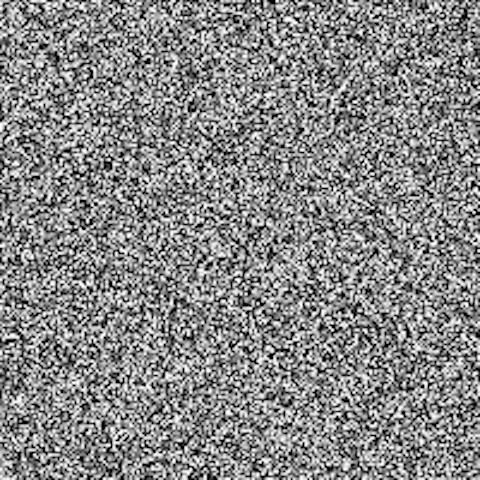
\includegraphics[scale=1.10]{WNoise200.png} & {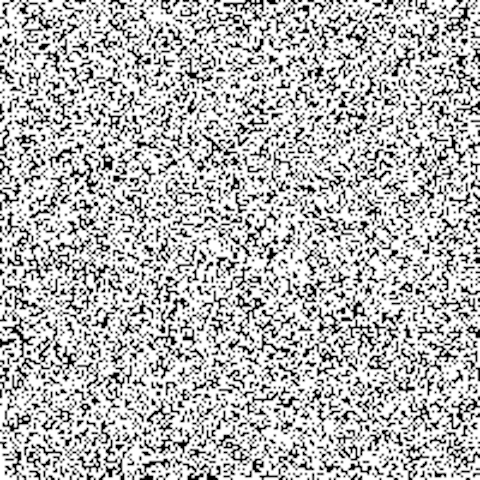
\includegraphics[scale=1.10]{WNoise200-t0382.png}} \\
{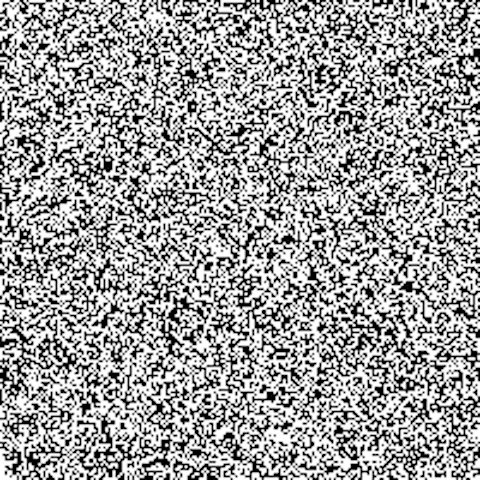
\includegraphics[scale=1.10]{WNoise200-t05.png}} & {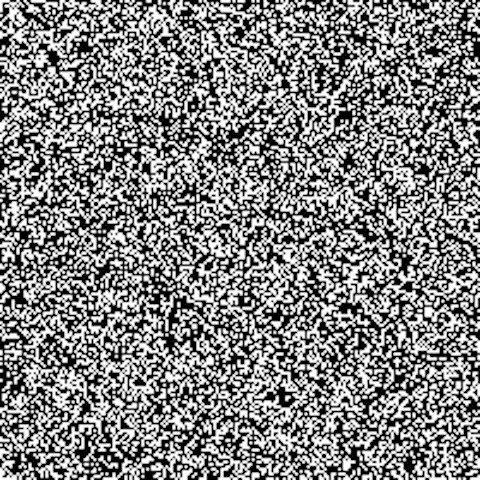
\includegraphics[scale=1.10]{WNoise200-t0618.png}}
\end{tabular}
\end{center}
\caption{First line: Left, a sample of a white noise with uniform distribution of size $200\times 200$ pixels; and right, excursion set for the level $t=\frac{1}{2}(3-\sqrt{5})$. Second line: excursion sets for the levels $t=\frac{1}{2}$ (left) and $\frac{1}{2}(-1+\sqrt{5})$ (right).}\label{WNoise:fig}
\end{figure}


\begin{figure}[!htbp]
\centering
\hfill
\begin{subfigure}
{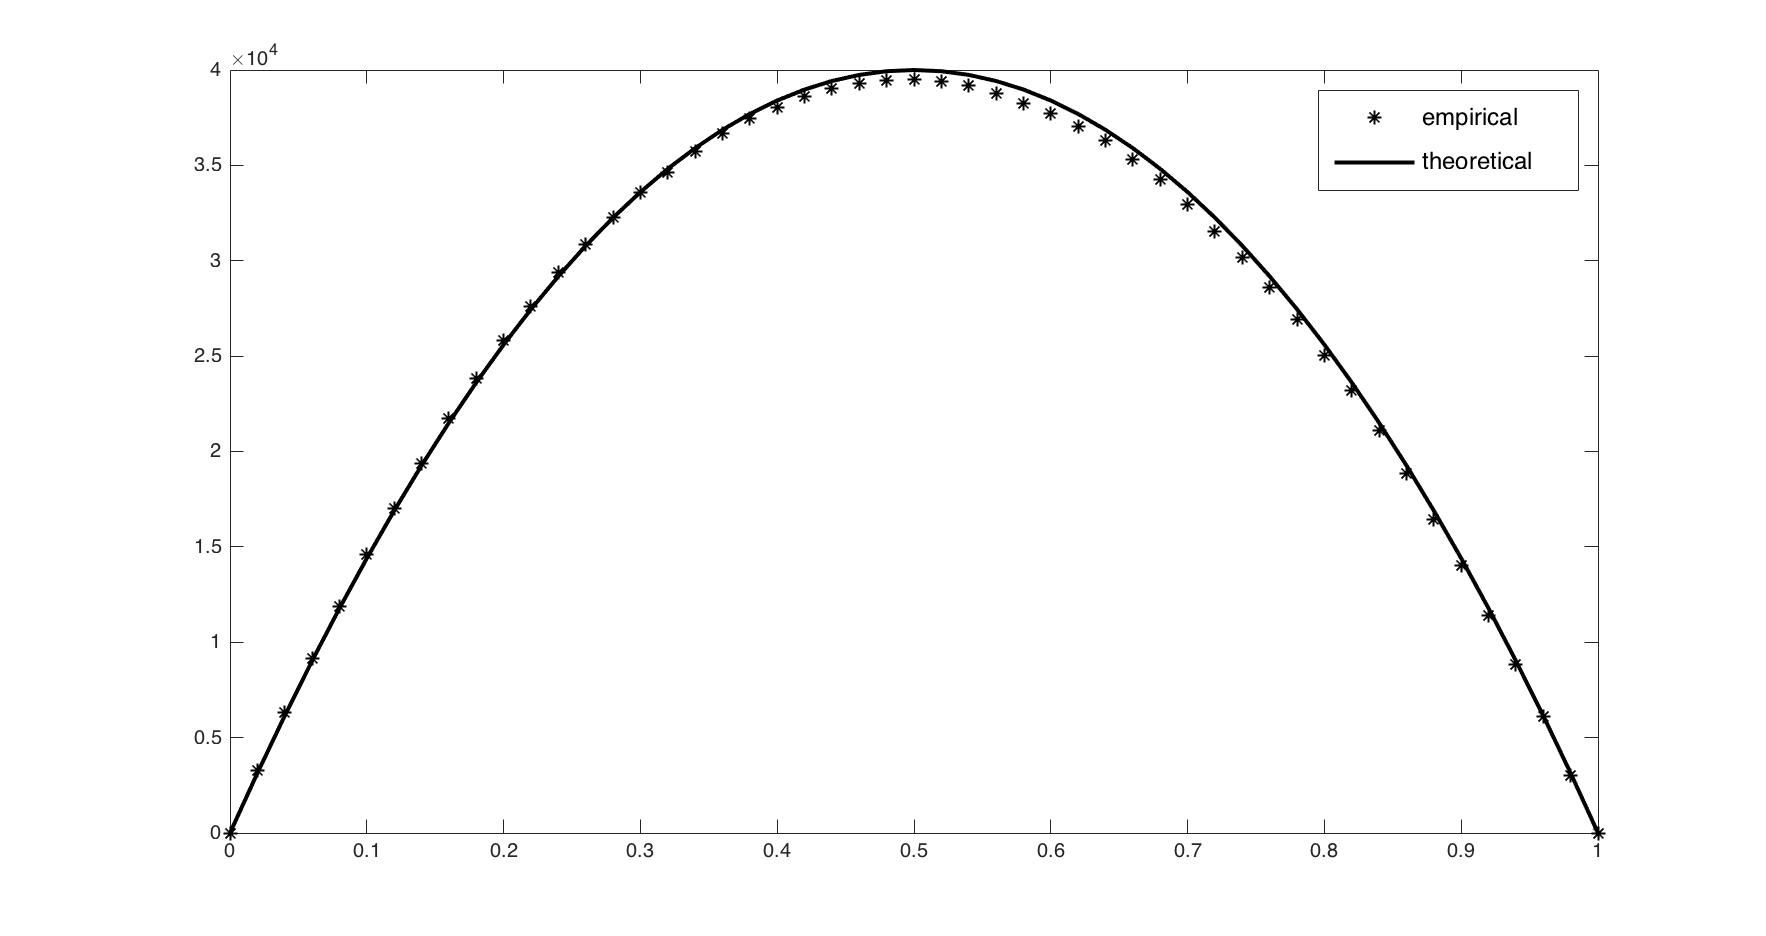
\includegraphics[scale=0.49]{LP-WNoise.png}}
\end{subfigure}
\hfill
\begin{subfigure}
{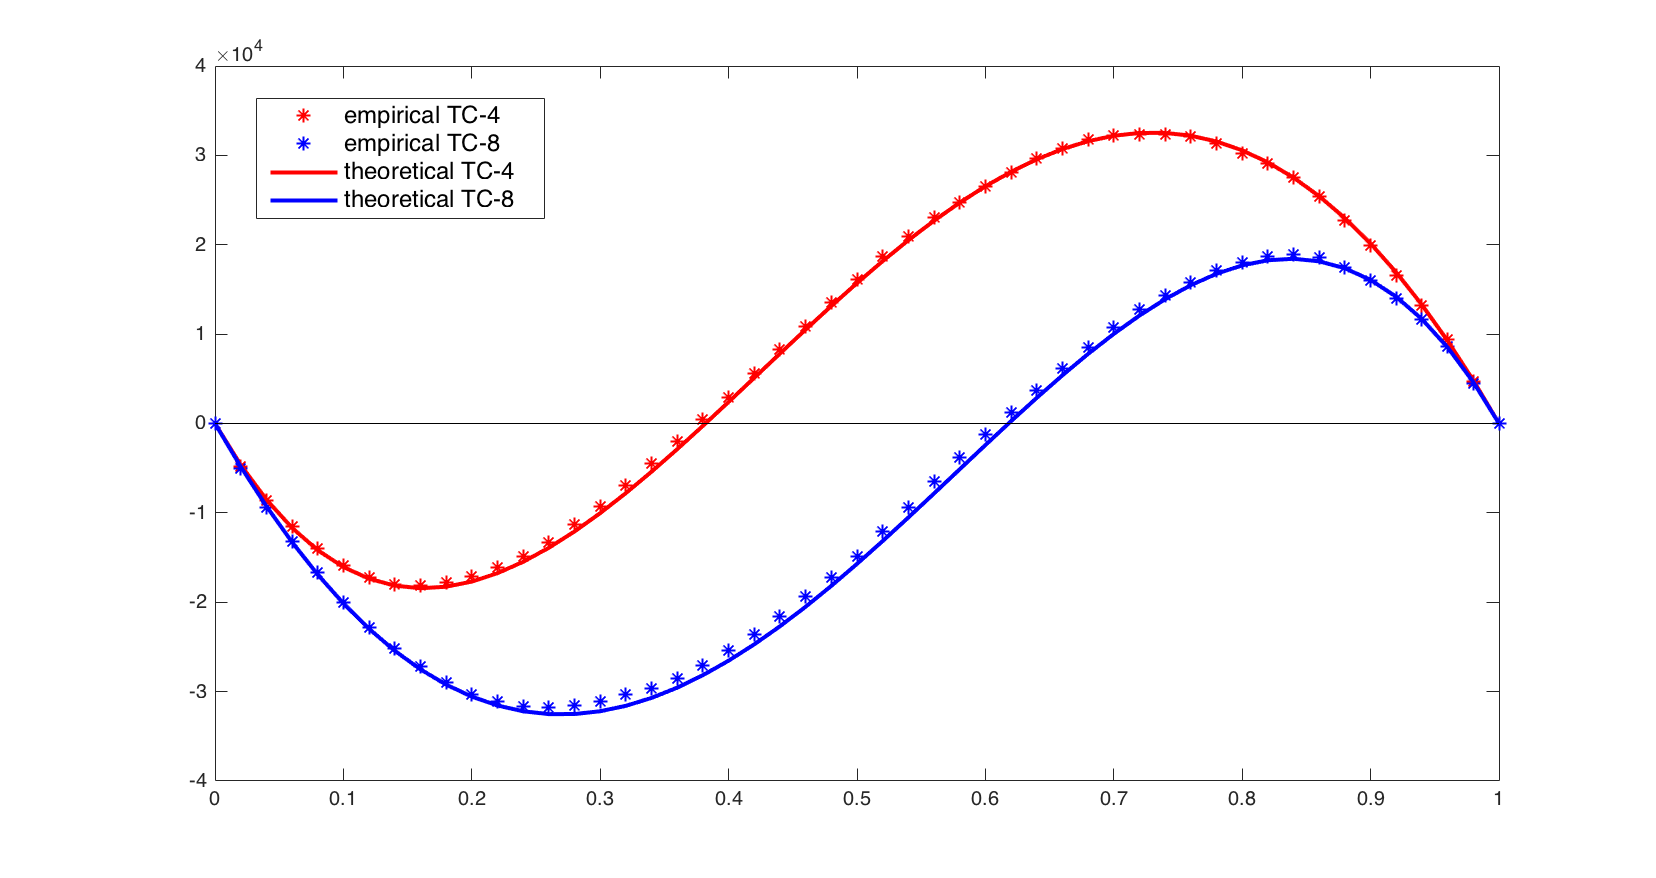
\includegraphics[scale=0.515]{LTC4-8-WNoise.png}}
\end{subfigure}
\caption{On the left, the perimeter of white noise with uniform distribution: empirical values (plotted with stars) and theoretical curve of the mean perimeter given by $t\mapsto \frac{4}{\eps^2} t(1-t) $. On the right, the total curvature: empirical values (plotted with stars) and theoretical mean total curvatures given by $t\mapsto \tfrac{2\pi}{\eps^2} t(1-t)[(2t-1) \pm\linebreak(1-t)t] $.}\label{LP-LTC-WNoise:fig}
\end{figure}

This example leads us to two remarks. The first one is that the empirical curves on one large sample are very close to the theoretical mean values, suggesting that the variances of $\LP_X$ and $\LTC_X$ are very small. Computing these variances is doable in theory and it would be an interesting direction for future investigations. The second remark is the question of knowing if there is a relationship between the values where $t\mapsto\E(\TC^\dd(\partial E_X(t,U_\eps))))$ crosses $0$ and percolation thresholds. Indeed in the hexagonal case, the percolation threshold is $p_c=0.5$ and this is also the value $t_c$ at which $t\mapsto \tfrac{2\pi}{\eps^2} t(1-t)(2t-1) $ crosses $0$. And in the square case, the percolation threshold is $p_c\simeq 0.593$ and $t_c= \tfrac{1}{2} + \tfrac{1-\sqrt{5}}{2} \simeq 0.618$ is the positive zero of $t\mapsto \E(\TC^4(\partial E_X(t),U_\eps))$, hence it seems that $|p_c-t_c|$ is ``small'', and studying this fact to know if it can be generalized would be interesting.



\subsection{Perimeter and total curvature of positively correlated Gaussian fields}\label{GaussianDiscret:sec}

It is more difficult to get explicit computations when considering non-independent random variables without adding assumptions on their distribution. In this section we consider the discretization of a standard centered Gaussian stationary field $X=\left(X(x)\right)_{x\,\in\,\R^2}$, that is also positively correlated, with covariance function $\rho$, meaning that $\Cov(X(x),X(y))=\rho(x-y)\ge 0$ with $\rho(0)=1$. Note that the case where the variance of $X(x)$, given by $\sigma^2 := \rho(0)$, is not equal to $1$ can easily be deduced from this one considering $X/\sigma$. For $\eps>0$ we consider the discretization of $X$ given by the set of the values $\left(X(z)\right)_{z\,\in\,\calC_\eps}$. The main quantities of interest will be
\begin{equation}\label{beta}
\beta_\theta(\eps) := \Var\left(X(\eps e_\theta)-X(0)\right)=2\left(1-\rho(\eps e_\theta)\right), \text{ for } e_\theta \in S^1.
\end{equation}

Note that the behavior of $\beta_\theta(\eps)$ is linked with the regularity of the field. Actually, mean square regularity is related to sample paths continuity for Gaussian fields (see~\cite{AdlerTaylorBook} for instance). Adding stationarity, one can deduce directional regularity from the behavior of $\beta_\theta(\eps)$ when $\eps$ tends to zero. For instance, when there exists $\alpha \in (0,1]$ and $\lambda_{2\alpha}(\theta)>0$ such that $\eps^{-2\alpha}\beta_\theta(\eps) \rightarrow
\lambda_{2\alpha}(\theta)$ as $\eps$ goes to $0$, one can find a modification of $X$ such that, for $x\in\R^2$, $t\in \R \mapsto X(x+t e_\theta)$ is almost surely $\alpha'$-H\"older continuous for any $\alpha'<\alpha$ (we refer the interested reader to~\cite[Part~2]{BGeosto}). Let us also emphasize that when $X$ is a.s. $C^1$ one has $\eps^{-2}\beta_\theta(\eps) \rightarrow \lambda_{2}(\theta)$, where $\lambda_{2}(\theta)=\Var(\partial_\theta X(0))$, with $\partial_\theta X $ the partial derivative of $X$ in the direction~$e_\theta$. When the field $X$ is isotropic this value does not depend on $\theta$ and the common value denoted as $\lambda_2$ is usually called second spectral moment.



In the following Theorem~\ref{GaussianDiscret:th} we focus on asymptotics for mean $\LP$ and $\LTC$ obtained for the discretization of $X$ on a tiling as $\eps$ goes to zero. Our results are mainly based on ordered statistics of order $2$ for $\LP$, $3$ for $\LTC$ in the hexagonal tiling case and $4$ for $\LTC$ in the square tiling case. Even with a Gaussian distribution, there are few results available in our dependent setting and we need to impose extra assumptions on the dependency given by the covariance function. In particular we are working with positively correlated variables meaning that $\rho$ is a non-negative function. Moreover, we will need the following assumptions:
\begin{enumerate}\Aenumi
\item \label{A1} there exists $\alpha\in (0,1]$ and real numbers $\lambda_{{2\alpha}}(\theta)\geq 0$ such that
\[
\eps^{-2\alpha}\beta_\theta(\eps)\underset{\eps\,\rightarrow\,0}{\longrightarrow} {\lambda_{{2\alpha}}(\theta)},
\]
for any edge orientation $e_\theta$ of the tiling.
\item \label{A2}Assumption~\eqref{A1} holds and $\rho(\eps e_\theta)=\rho(\eps e_{\pi/2})$ for any edge orientation $e_\theta$ of the tiling, hence we write $\lambda_{{2\alpha}}$ the common value of $\lambda_{{2\alpha}}(\theta)$.
\item \label{A3}Assumption~\eqref{A2} holds for the square tiling and $\rho(\eps e_{\pi/2})-\rho(\eps (e_0+e_{\pi/2}))> 0$ and $1-2\rho(\eps e_{\pi/2})+\rho(\eps (e_0+e_{\pi/2}))\ge 0$ with
\[
\eps^{-2\alpha}\big(1-2\rho(\eps e_{\pi/2})+\rho(\eps
(e_0+e_{\pi/2}))\big) \underset{\eps\,\rightarrow\,0}{\longrightarrow} 0.
\]
\end{enumerate}


\begin{theo}\label{GaussianDiscret:th}
We consider the discretization $X_\eps$ of a centered stationary standard Gaussian and positively correlated random field $X$. Let $h \in C_b(\R)\cap L^1(\R)$.

\noindent Then, under~\eqref{A1},
\[
\left(\sqrt{3}\eps\right)^{(1-\alpha)}\E\left(\LP_{X_\eps^{\Hex}}(h,U_\eps)\right)\underset{\eps\,\rightarrow\,0}{\longrightarrow}{\calL}(U)\times \frac{2}{{\pi}}
\left(\frac{1}{3}\sum_{i=1}^3\sqrt{{\lambda_{{2\alpha}}(\theta_i)}}\right)\int_{\R}h(t)e^{-t^2/2}dt,
\]
with $\{\theta_i;1\le i\le 3\}=\{\pi/2,\pm\pi/6\}$, while
\[
\eps^{(1-\alpha)}\E\left(\LP_{X_\eps^{\Sq}}(h,U_\eps)\right)\longrightarrow
{\calL}(U)\times \frac{2}{{\pi}} \left(\frac{1}{2}\sum_{i=1}^2\sqrt{{\lambda_{{2\alpha}}(\theta_i)}}\right)\int_{\R}h(t)e^{-t^2/2}dt,
\]
with $\{\theta_1,\theta_2\}=\{0,\pi/2\}$.\\
Moreover, under~\eqref{A2},
\[
\left(\sqrt{3}\eps\right)^{2(1-\alpha)}\E\left(\LTC_{X_\eps^{\Hex}}(h,U_\eps)\right)\underset{\eps\,\rightarrow\,0}{\longrightarrow} {\calL}(U)\times\frac{1}{\sqrt{2\pi}}\lambda_{{2\alpha}}\int_{\R}h(t)te^{-t^2/2}dt.
\]
Finally, under~\eqref{A3}, then
\[
\eps^{2(1-\alpha)}\E\left(\LTC^6_{X_\eps^{\Sq}}(h,U_\eps)\right)\underset{\eps\rightarrow 0}{\longrightarrow} {\calL}(U)\times
\frac{1}{\sqrt{2\pi}}\lambda_{{2\alpha}}\int_{\R}h(t)te^{-t^2/2}dt,
\]
where we recall that $\LTC^6:=\frac{1}{2}(\LTC^4+ \LTC^8)$.
\end{theo}

The proof of this theorem is technical and it is postponed to Appendix~\ref{App:GaussianDiscret:th}


\begin{rema}
When $X$ is assumed to be a.s. $C^3$ and isotropic, we have for all $t\in\R$,
\[
\E\left(\Per(E_X(t),U)\right) =2{\calL}(U)C_1^\ast(X,t)\;\text{ and }\;
\E\left(\TC(\partial E_X(t)\cap U)\right)= 2\pi {\calL}(U) C_0^\ast(X,t),
\]
where $C_1^\ast$ and $C_0^\ast$ are the Lipschitz--Killing curvatures densities (see~\cite{BDDE-19}), given by
\[
C_1^\ast(X,t)=\frac{1}{4}\sqrt{\lambda_2}e^{-t^2/2} \quad \text{ and
} \quad C_0^\ast(X,t)=(2\pi)^{-3/2}{\lambda_2}te^{-t^2/2},
\]
where $\lambda_2$ denotes the spectral moment of $X$ corresponding to $\Var(\partial_1 X(0))\linebreak=\Var(\partial_2 X(0))$ by isotropy. Since
\[
\Var\left(\partial_j X(0)\right)=\lim_{\eps\rightarrow 0}\Var\left(\frac{X(\eps e_{\theta_j})-X(0)}{\eps}\right)=\lim_{\eps\rightarrow 0}\eps^{-2}\beta_{\theta_j}(\eps),\text{ for }\theta_1=0
\,
\text{ and }\theta_2=\frac{\pi}{2},
\]
the field $X$ will satisfy~\eqref{A1} with $\alpha=1$ and $\lambda_{2\alpha}(\theta)=\lambda_2$ for any orientation $\theta$ by isotropy, as soon as $\rho$ is non-negative in order to ensure the positive dependence assumption. Hence, since it also satisfies~\eqref{A2} by isotropy, by Theorem~\ref{GaussianDiscret:th} we obtain for any $h\in C_b(\R)\cap L^1(\R)$,
\begin{align*}
\E\left(\LP_{X_\eps^{\Hex}}(h,U_\eps)\right)&\underset{\eps\,\to\,
0}{\longrightarrow}\frac{4}{\pi}\times \E(\LP_X(h,U)) \\
\text{ and }
\E\left(\LTC_{X_\eps^{\Hex}}(h,U_\eps)\right)&\underset{\eps\,\to\,0}{\longrightarrow} \E(\LTC_X(h,U)),
\end{align*}
with
\begin{align*} 
\E\left(\LP_X(h,U)\right) &=\int_\R h(t)\E\left(\Per(E_X(t),U)\right) dt
\\
\text{ and } \E\left(\LTC_X(h,U)\right) &=\int_\R h(t) \E\left(\TC(\partial E_X(t)\cap U)\right) dt.
\end{align*}
It follows that we have a weak-convergence
\begin{align*}
\E\left(\Per\left(E_{X_\eps^{\Hex}}(t),U_\eps\right)\right) &\underset{\eps\,\to\,0}{\rightharpoonup} \frac{4}{\pi}\times \E\left(\Per(E_X(t),U)\right)
\\
\text{ and }
\E\left(\TC\left(\partial E_{X_\eps^{\Hex}}(t)\cap U_\eps\right)\right) &\underset{\eps\to 0}{\rightharpoonup}
\E\left(\TC(\partial E_X(t) \cap U)\right).
\end{align*}
\end{rema}

Now, if we assume moreover that $\rho(x)=\tilde{\rho}(\|x\|^2)$ with $\tilde{\rho}$ a non-negative function that is $C^2$ on a neighbourhood of $0$ and such that $\tilde{\rho}'(0)<0$ and $\tilde{\rho}''(0)>0$ we easily check, using Taylor formula, the additional assumptions for the square tiling and also obtain the weak-convergence
\begin{align*}
\E\left(\Per\left(E_{X_\eps^{\Sq}}(t),U_\eps\right)\right) &\underset{\eps\,\to\, 0}{\rightharpoonup} \frac{4}{\pi}\times \E\left(\Per\left(E_X(t),U\right)\right)
\\
\text{ and }
\E\left(\TC^6\left(\partial E_{X_\eps^{\Sq}}(t)\cap U_\eps\right)\right) &\underset{\eps\,\to\,0}{\rightharpoonup} \E\left(\TC\left(\partial
E_X(t)\cap U\right)\right).
\end{align*}
An example of such a field is given choosing $\tilde{\rho}(r)=e^{-\kappa^2 r}$, for some $\kappa>0$, such that $\lambda_2=2\kappa^2$. Note that the over-estimation for the perimeter, as remarked in~\cite[Figure~1]{BDDE-19}, is now corrected with the multiplication by $\frac{4}{\pi}$ for the theoretical value. This is illustrated in Figure~\ref{StatGaussT100:fig} where we have chosen $\rho(x)=e^{-\kappa^2\|x\|^2}$ for $\kappa=100$, $U=(0,1)^2$ and $\eps=2^{-10}$ (that could also correspond to $(0,100)^2$, $\kappa=1$ and $\eps=100\times 2^{-10}$).

\begin{figure}[!b]
\centering
\hfill
\begin{subfigure}
{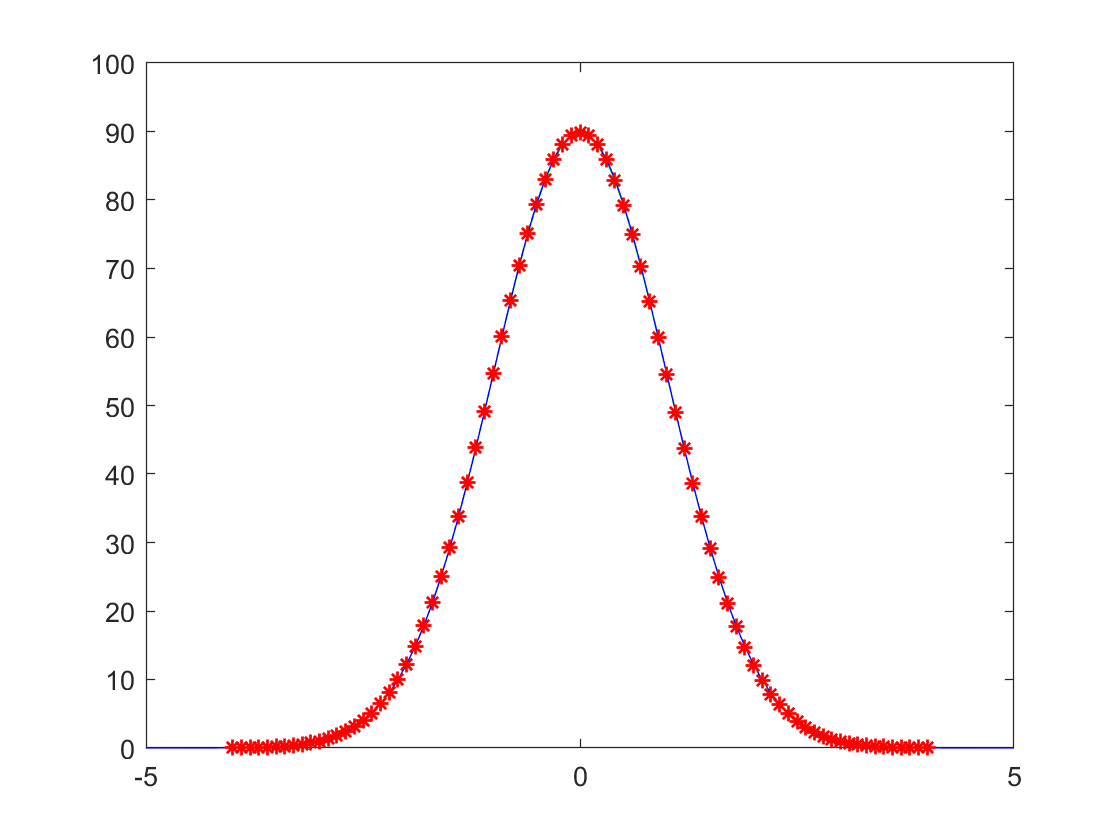
\includegraphics[scale=0.76]{PerGaussT100.png}}
\end{subfigure}
\hfill
\begin{subfigure}
{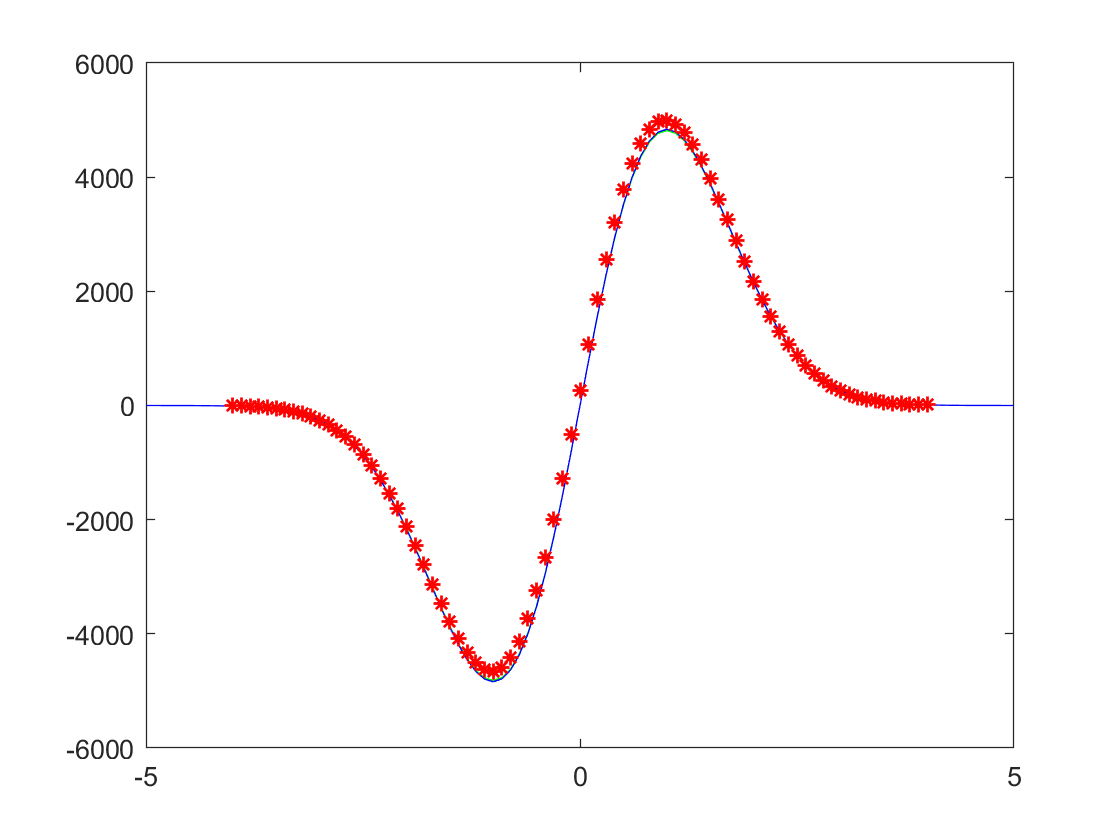
\includegraphics[scale=0.76]{TCGaussT100.png}}
\end{subfigure}
\caption{Smooth isotropic correlated Gaussian field. Left: Perimeter, empirical values plotted with red stars and theoretical curves of the mean perimeter given by $t\mapsto \tfrac{2}{\pi}\sqrt{\text{\small{$\lambda_2$}}}e^{-t^2/2} $ in blue and $t\mapsto
\tfrac{2}{\pi}\sqrt{\text{\small{$\eps^{-2}\beta_0(\eps)$}}}e^{-t^2/2}$ in green. Right: Total curvature $\TC^6=\tfrac{1}{2}(\TC^4+\TC^8)$, empirical values plotted with red stars and theoretical mean total curvatures given by $t\mapsto \tfrac{1}{\sqrt{2\pi}} \lambda_2te^{-t^2/2}$ in blue and $t\mapsto \tfrac{1}{\sqrt{2\pi}} \eps^{-2}\beta_0(\eps)te^{-t^2/2}$ in green. }\label{StatGaussT100:fig}
\end{figure}


We can also illustrate Theorem~\ref{GaussianDiscret:th} with some fractional fields that are not $C^1$ anymore. Let us take for example the covariance function $\rho(x)=e^{-\kappa^{2\alpha} \|x\|^{2\alpha}}$ for $\alpha \in (0,1)$. For such a covariance function, the results on the hexagonal tiling will hold with $\lambda_{2\alpha}(\theta)=2\kappa^{2\alpha}$. However even if we have $\rho(\eps e_{\pi/2})-\rho(\eps (e_0+e_{\pi/2})\ge 0$ we get $1-2\rho(\eps e_{\pi/2})+\rho(\eps (e_0+e_{\pi/2}))=(2^{\alpha}-2)\eps^{2\alpha}(\kappa^{2\alpha}+o(1))$. Hence the square tiling assumption for the total curvature~\eqref{A3} fails in this case. Choosing instead an anisotropic covariance function given by $\rho(x)=e^{-\kappa^{2\alpha} (x_1^{2\alpha} + x_2^{2\alpha})}$ for $x=(x_1,x_2)\in\R^2$, is enough to check all needed assumptions~\eqref{A1}, \eqref{A2} and~\eqref{A3}. We illustrate this for the square tiling with $\alpha=0.5$ on Figures~\ref{Exp05T100:fig} and~\ref{StatExp05T100:fig}. Here we consider $U=(0,1)^2$, $\kappa=100$ and $\eps=2^{-10}$ (that could also correspond to $U=(0,100)^2$, $\kappa=1$ and $\eps=100\times 2^{-10}$).



\begin{figure}[!h]
%\begin{center}
%[width=6cm]
%\begin{tabular}{ll}
\centering
\begin{subfigure}
{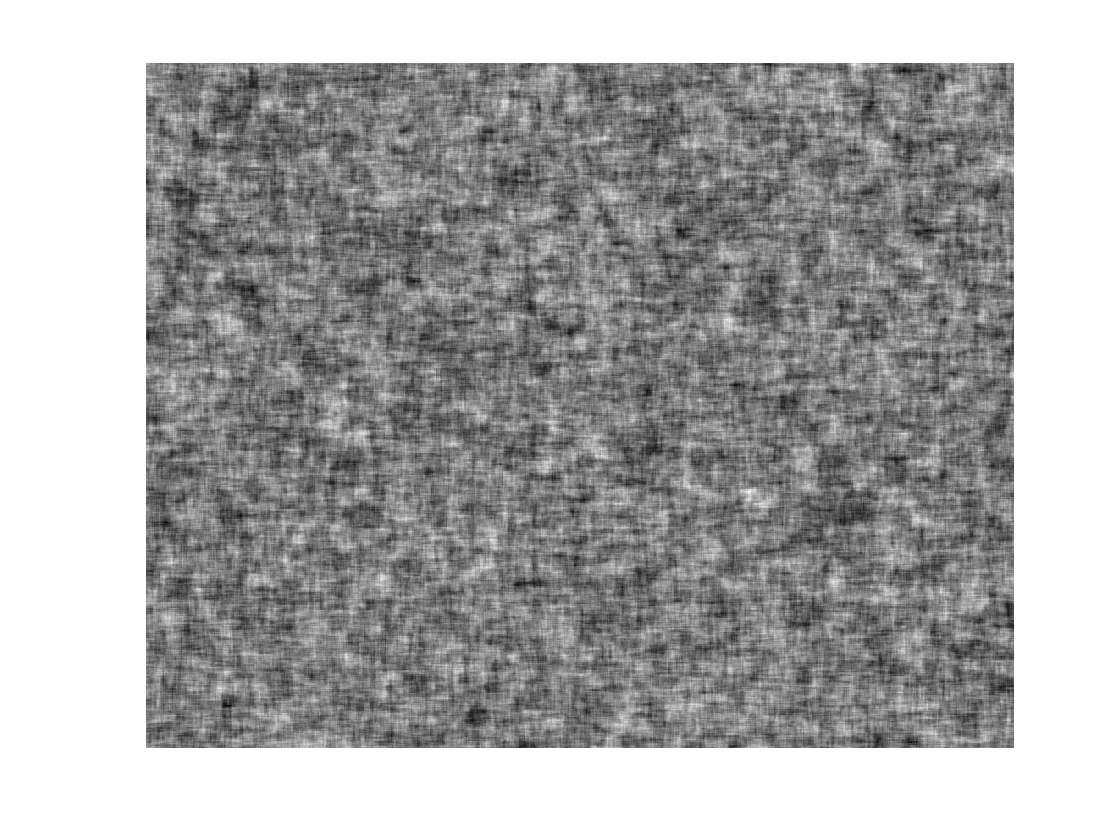
\includegraphics[scale=0.68]{Exp05T100.png}}
\end{subfigure}
\hspace{0.5mm}
\begin{subfigure}
 {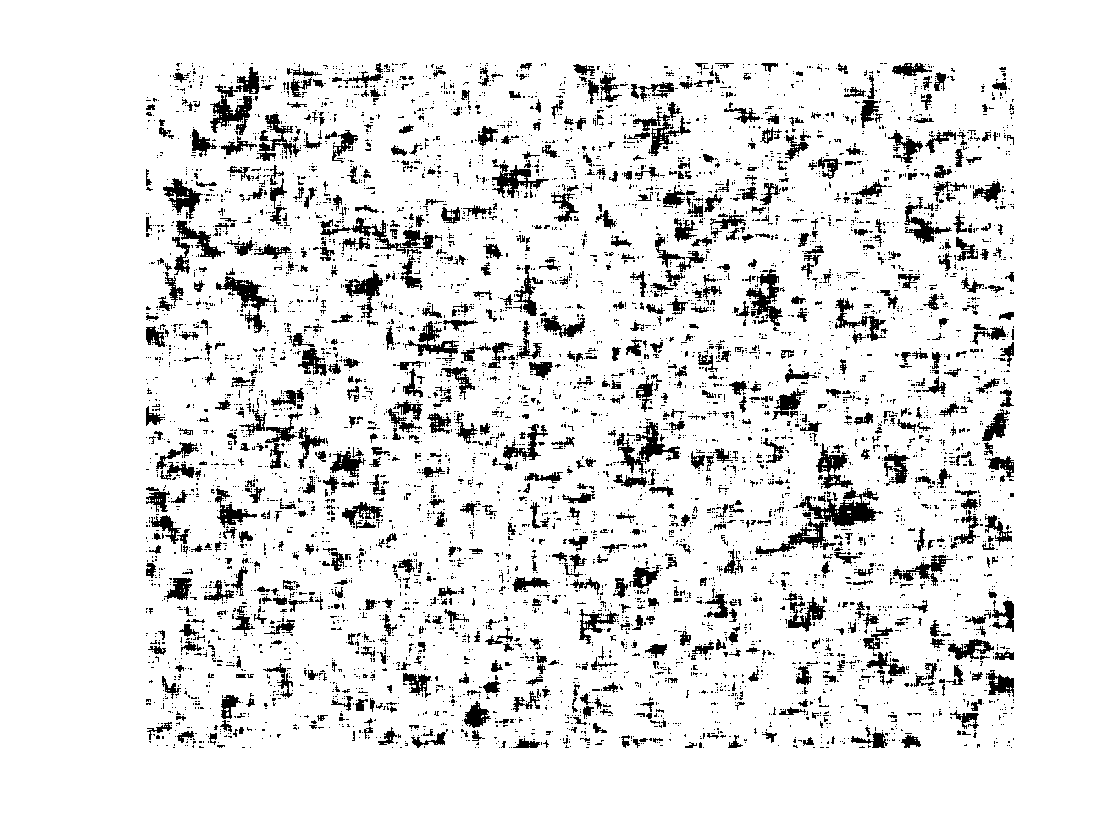
\includegraphics[scale=0.68]{ExcminExp05T100.png}}
\end{subfigure}\\[-1.5em]
\begin{subfigure}
{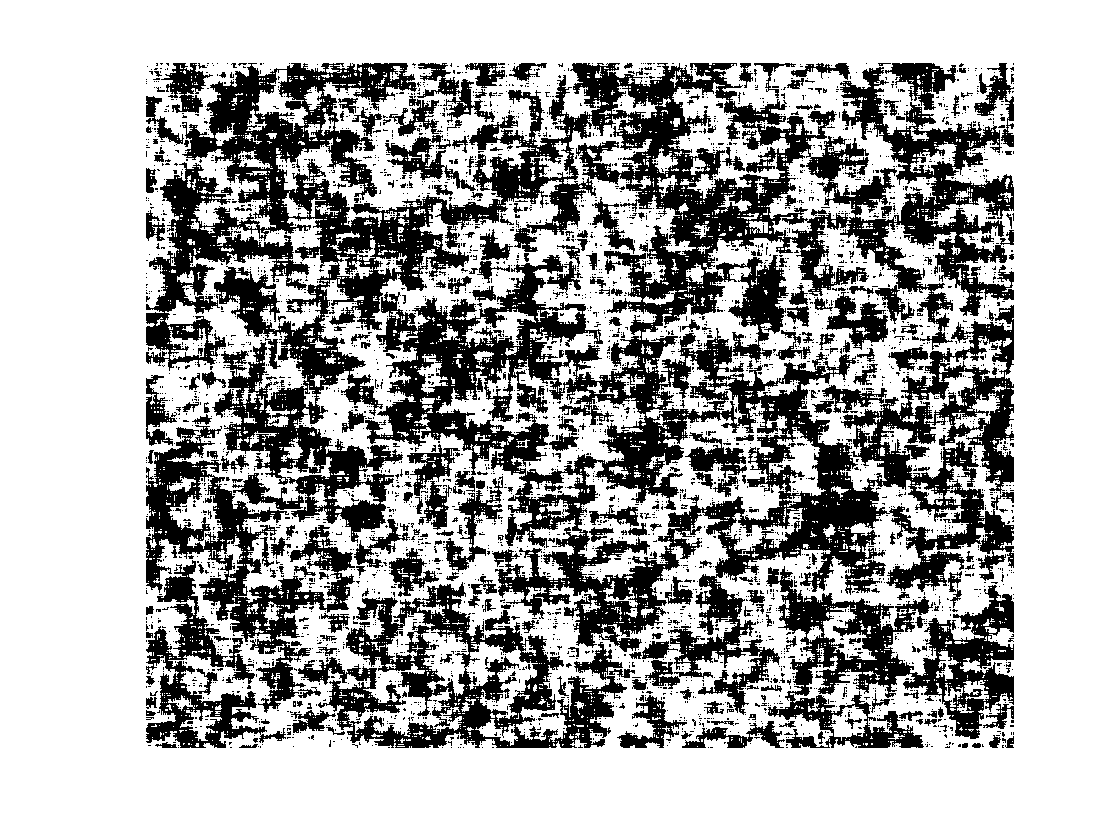
\includegraphics[scale=0.68]{ExcmidExp05T100.png}}
\end{subfigure}
\hspace{0.5mm}
\begin{subfigure}
 {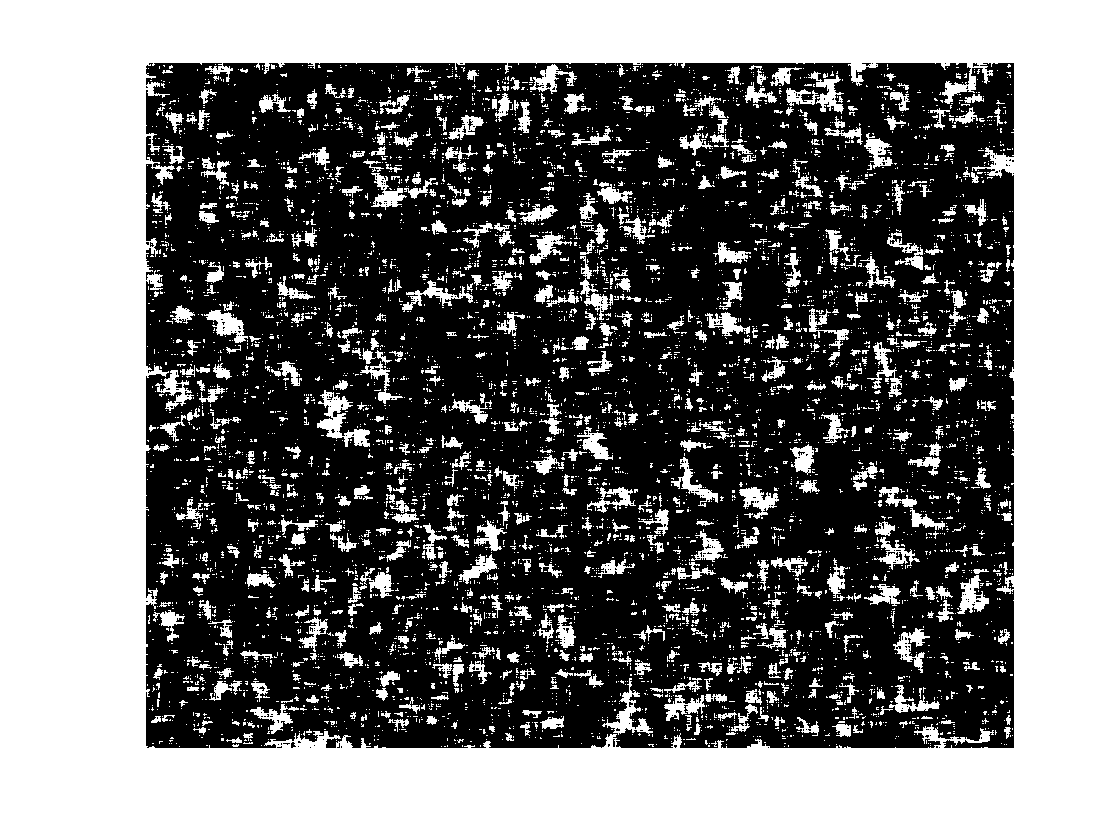
\includegraphics[scale=0.68]{ExcmaxExp05T100.png}}
 \end{subfigure}
%\end{tabular}
%\end{center}
\caption{First line: Left, a sample of a fractional correlated standard Gaussian field of size $2^{10}\times 2^{10}$ pixels for $\alpha=0.5$; and right, excursion set for the level $t=-1$. Second line: excursion sets for the levels $t=0$ (left) and $1$ (right).}\label{Exp05T100:fig}
\end{figure}

\begin{figure}[!htbp]
\centering\hfill
\begin{subfigure}
{\!\!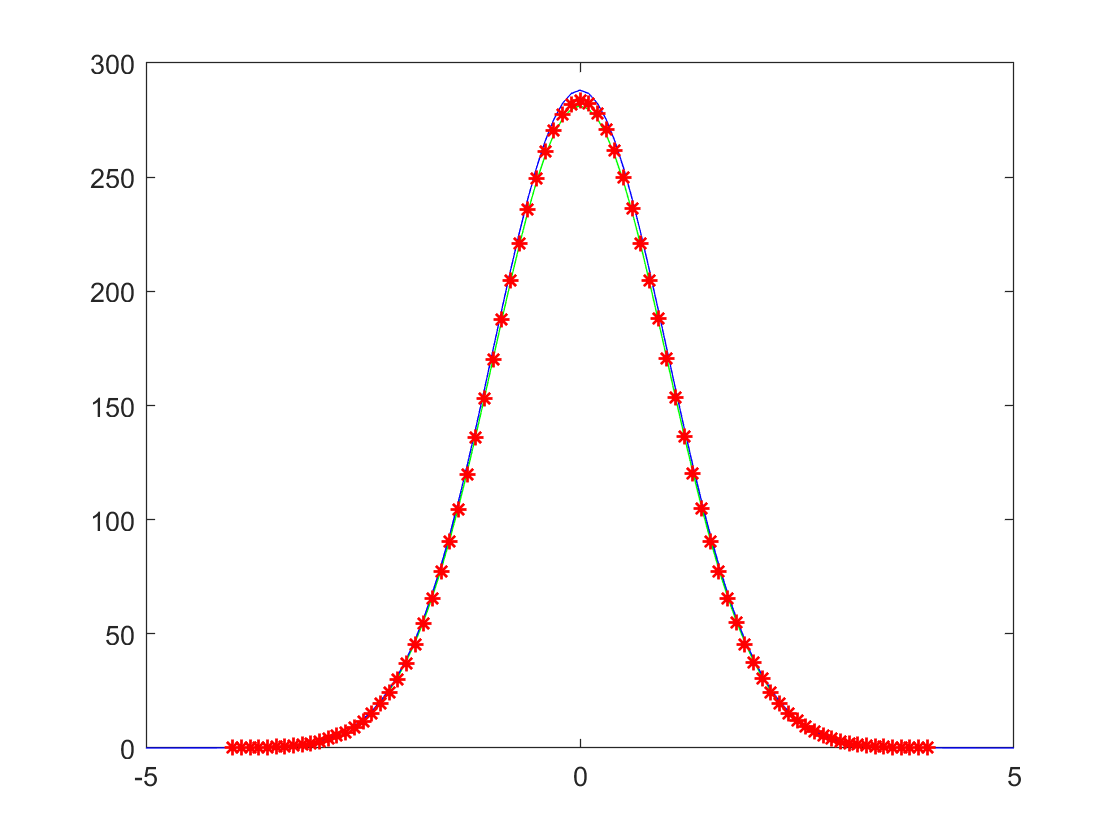
\includegraphics[scale=0.75]{PerExp05T100.png}}
\end{subfigure}
\hfill
\begin{subfigure}
{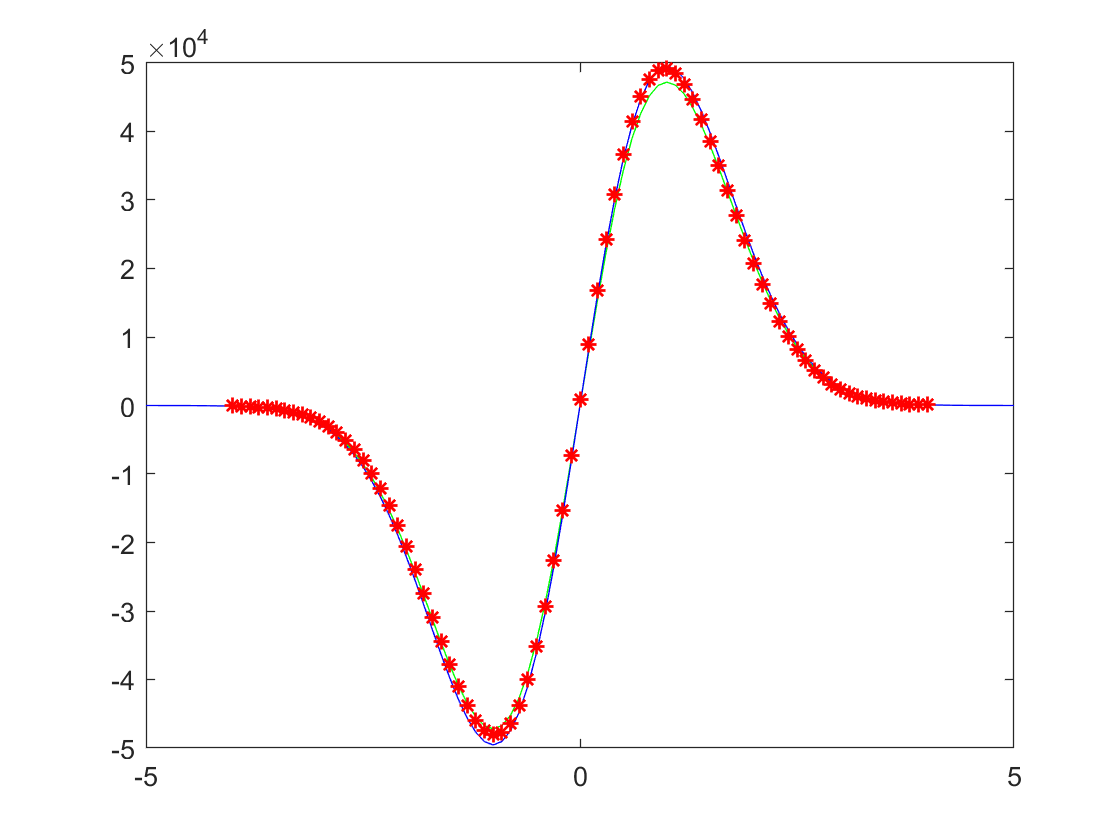
\includegraphics[scale=0.75]{TCExp05T100.png}}
\end{subfigure}
\caption{Fractional correlated Gaussian field for $\alpha=0.5$. Left: Perimeter, empirical values (red stars) and theoretical curves of the mean perimeter given by $t\mapsto \eps^{-(1-\alpha)}\tfrac{2}{\pi}\sqrt{\text{\small{$\lambda_{2\alpha}$}}}e^{-t^2/2} $ in blue and $t\mapsto
\tfrac{2}{\pi}\sqrt{\text{\small{$\eps^{-2}\beta_0(\eps)$}}}e^{-t^2/2}$ in green. Right: Total curvature $\TC^6=\tfrac{1}{2}(\TC^4+\TC^8)$, empirical values (red stars) and theoretical mean total curvatures given by $t\mapsto \eps^{-2(1-\alpha)}\tfrac{1}{\sqrt{2\pi}} \lambda_{2\alpha}te^{-t^2/2}$ in blue and $t\mapsto \tfrac{1}{\sqrt{2\pi}} \eps^{-2}\beta_0(\eps)te^{-t^2/2}$ in green. }\label{StatExp05T100:fig}
\end{figure}



We also illustrate the resolution effect on Figure~\ref{resolution:fig} where we still consider\linebreak$U=(0,1)^2$ given with a maximal resolution (minimal $\eps$) $\eps_{min}=2^{-10}$ for $2^{10}\times 2^{10}$ pixels and discretize the field for intermediate resolution $\eps=2^{-k}$, for $k\in\{6,7,8\}$ and $\alpha=0.5$. Finally, Figure~\ref{TVresal:fig} presents in $\log$-$\log$ scale the dependency of the computation of the total variation $\LP_{X_\eps}(U)=\int_\R\Per(E_{X_\eps}(t),U)dt$ (computed by a Riemann sum for empirical values) compared to the theoretical values given with the normalized spectral moment $\eps^{2\alpha}\lambda_{2\alpha} $ or considering the non asymptotic spectral moment given by $\beta_0(\eps)=2(1-\exp(-(\kappa\eps)^{\alpha})$. Actually, if we could take $h=1$ in Theorem~\ref{GaussianDiscret:th}, we should observe $\LP_{X_\eps}(U)\sim 2\sqrt{\text{\small{$\tfrac{2\lambda_{2\alpha}}{\pi}$}}}\eps^{-(1-\alpha)}=2\sqrt{\text{\small{$\tfrac{2}{\pi}$}}}\eps^{-1}\sqrt{\eps^{2\alpha}\lambda_{2\alpha}}.$ We can observe the $1-\alpha$ slope for $\log$-$\log$ scale in Figure~\ref{TVresal:fig} but it seems also that $\E(\LP_{X_\eps}(U))\sim 2\sqrt{\text{\small{$\frac{2}{\pi}$}}}\eps^{-1}\sqrt{\text{\small{$\beta_0(\eps)$}}}$ gives a better estimate for smaller resolution. For total curvature, we compute similarly the Riemann sum of the absolute empirical values and we denote $\LaTC_X(U)=\int_{\R}|\TC(\partial E_X(t)\cap U)|dt$. Now the slopes are given by $2(1-\alpha)$ and similarly, a better match is obtained choosing $\beta_0(\eps)$ instead of $\eps^{2\alpha}\lambda_{2\alpha}$ in the theoretical formula.

\begin{figure}[!htbp]
\centering
\hfill
%[width=5cm]
\begin{subfigure}[$\eps=2^{-8}$]
{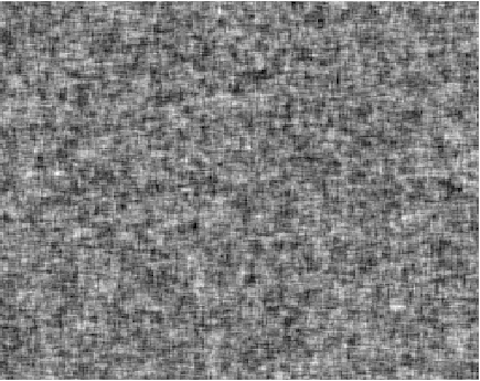
\includegraphics{Imdiscal05eps8-2.png}}
\end{subfigure}
\hfill
\begin{subfigure}[$\eps=2^{-7}$]
{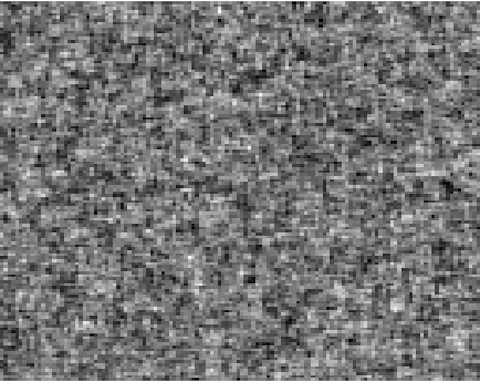
\includegraphics{Imdiscal05eps7-2.png}}
\end{subfigure}
\hfill
\begin{subfigure}[$\eps=2^{-6}$]
{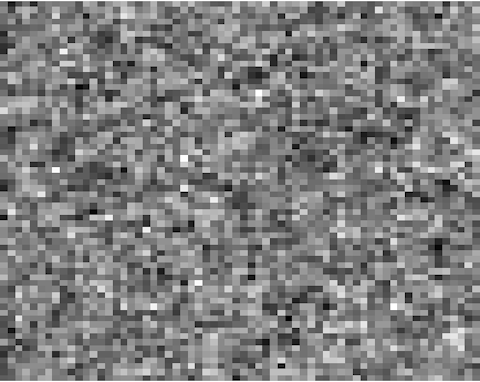
\includegraphics{Imdiscal05eps6-2.png}}
\end{subfigure}
\caption{A sample of a fractional correlated standard Gaussian field of size $2^{10}\times 2^{10}$ pixels for $\alpha=0.5$ and different resolutions $\eps$.}\label{resolution:fig}
\vspace{-6pt}
\end{figure}
%\begin{tabular}{ccc}
%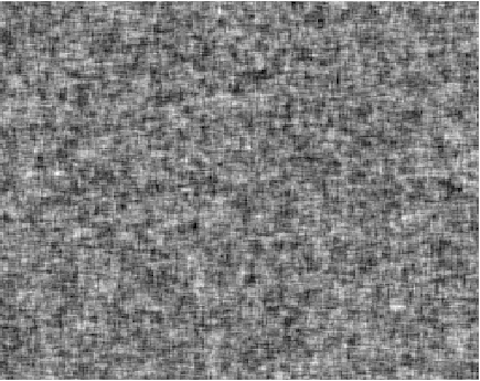
\includegraphics[width=5cm]{Imdiscal05eps8-2.png} & {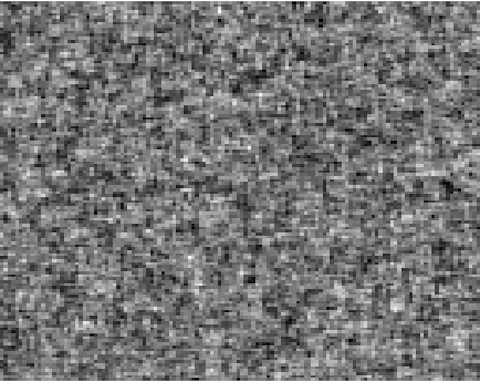
\includegraphics[width=5cm]{Imdiscal05eps7-2.png}} & {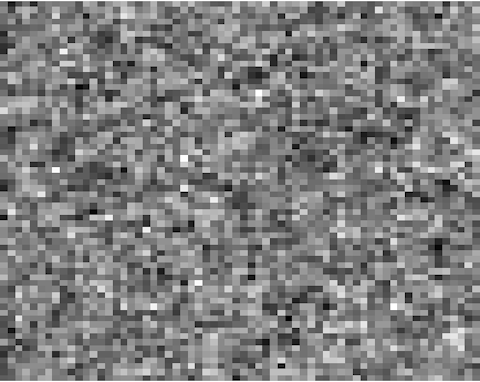
\includegraphics[width=5cm]{Imdiscal05eps6-2.png}} \\
%$\eps=2^{-8}$& $\eps=2^{-7}$&$\eps=2^{-6}$
%\end{tabular}
%\end{center}


\begin{figure}
%\begin{center}
%\begin{tabular}{cc}
\centering
\hfill
\begin{subfigure}
{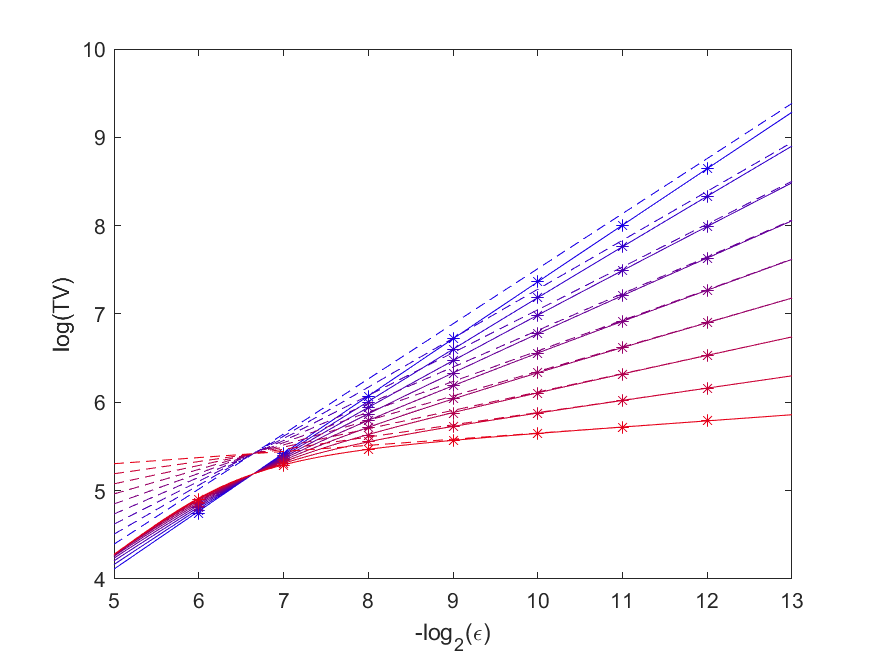
\includegraphics[scale=0.98]{VTresal.png}}
\end{subfigure}
\hfill
\begin{subfigure}
{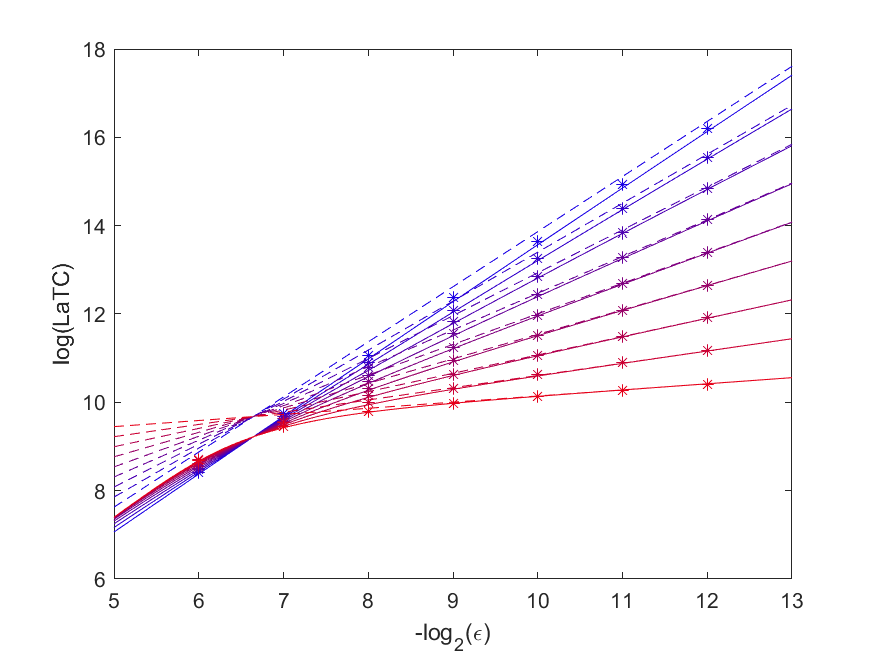
\includegraphics[scale=0.98]{LaTCresal.png}}
\end{subfigure}
%%\end{tabular}
%\end{center}
\caption{Log-log plots of $\TV$ and $\LTaC$ for fractional correlated standard Gaussian fields of size $2^{12}\times 2^{12}$ pixels for $\alpha$ varying between $0.1$ (in blue) and $0.9$ (in red), as functions of the resolution $\eps$. Empirical values are plotted with stars and theoretical ones are plotted with dashed curves for $\eps^{2\alpha}\lambda_{2\alpha}$ and with continuous curves for $\beta_0(\eps)$.}\label{TVresal:fig}
\end{figure}


\break
\section{Discretization of smooth functions}\label{DoSF:sec}

In this section, we will study the limits of $\LP_{f_\eps}$ and $\LTC_{f_\eps}$ as the size $\eps$ of the tiling goes to $0$, when $f$ is a smooth function. In particular, we would like to know if the limits coincide with $\LP_f$ and $\LTC_f$. For this aim, let $U=(0,T)^2$ with $T>0$ and we recall first the main formulas obtained in our previous paper~\cite{BD-Geometry-published} for a smooth ($C^2$) function $f$ on $\R^2$, given by~\eqref{LPfsmooth:eq} and~\eqref{LTCfsmooth:eq}, for $h\in C_b(\R)$.


When $h$ is also assumed to be $C^1$ on $\R$, denoting by $H$ a primitive of $h$, a simple computation leads to, for any vector $e\in\R^2$, 
\[
D^2(H\circ f)(x).(e,e) = h'(f(x))\left\langle \nabla f(x),e\right\rangle^2 +
h(f(x)) D^2 f(x).(e,e),
\]
where $\langle \cdot,\cdot\rangle$ is the Euclidean scalar product on $\R^2$. Using this formula with $e=\tfrac{\nabla f(x)^\perp}{|\nabla f(x)|} $, we get, 

\begin{align*}
\LTC_f (h,U) & = - \int_U D^2(H\circ f)(x).\left(\frac{\nabla f(x)^\perp}{\left|\nabla f(x)\right|}, \frac{\nabla f(x)^\perp}{\left|\nabla f(x)\right|} \right) \ind_{\left|\nabla\,(H\circ f)\,(x)\right|\,>\,0} \, dx \\
&= \LTC_{H\,\circ\,f} (1,U) = \LTC_{H\,\circ\,f} (U).
\end{align*}
Hence we are reduced back to the case $h=1$. In a similar way, decomposing a bounded continuous function $h$ into $h=h_1-h_2$, where $h_1=h +2 \|h\|_\infty$ and $h_2=2 \| h\|_\infty$ are both positive continuous and bounded functions, we get that
\[
\LP_f (h,U) = \LP_{H_1\circ f} (U)-\LP_{H_2\circ f} (U).
\]
Observe that we also have $\LP_f (h,U_\eps) = \LP_{H_1\circ f} (U_\eps)-\LP_{H_2\circ f} (U_\eps),$ when $f\in\PC^{\Hex}_\eps(U^{\eps})$ or $f\in \PC^{\Sq}_\eps(U^{\eps})$. Since we can proceed similarly for the level total curvature we will focus on the case where $h=1$ in the following.

%\medskip
%
%
%\smallskip

Usually, to infer an approximation error between the integral of a function and its discretized version, one uses an approximation inequality like the Koksma--Hlawka inequality~\cite{PausingerSvane2015}. Now here we will need a similar result that is given by the following proposition.

\begin{prop}[Approximation Inequality]\label{approx:prop}
Let $W$ be a rectangular domain in $\R^2$. Let $g$ be a bounded, Lipschitz function defined on $\R^2$. Let us consider a regular tiling with a shape $H_\eps$ (that can be an hexagon, a square or a rhomb) of ``size'' $\eps$. Let $a_\eps=\calL(H_\eps)$ be the area of $H_\eps$ and let $d_\eps$ be the diameter of $H_\eps$ (that is the maximal distance between two points of $H_\eps$). Let $\calC_\eps$ be the set of centers of the tiles. Then
\begin{multline*}
\left| a_\eps \sum_{y\,\in\,\calC_\eps \,\cap\,W } g(y) - \int_W g(x) \, dx
\right|
\\
\leq d_\eps \left(\calL(W) \Lip(g) + 2 \calH^1(\partial W)
\sup |g|\right) + d_\eps^2 \Lip(g) L\left(\calH^1(\partial W) + 4 d_\eps\right).
\end{multline*}

Let $A\subset W$ be an open or closed subset of $W$. Then the cardinality of $\calC_\eps \cap A$ is bounded:
\[
\left| \calC_\eps \cap A \right| \leq \frac{1}{a_\eps} \calL \left(A
\oplus B(0,d_\eps)\right),
\]
where $B(0,d_\eps)$ is the ball of center $0$ and radius $d_\eps$, and $\oplus$ denotes the Minkowski sum, defined by $A\oplus B := \{x+y \, ; \, x\in A \text{ and } y\in B\}$.
\end{prop}

\begin{proof}
Let us start with the first part of the proposition. We notice that
\[
a_\eps \sum_{y\,\in\,\calC_\eps\,\cap\,W } g(y) = \sum_{y\,\in\,\calC_\eps\,
\cap\,W } \int_{H_\eps} g(y) \, dz.
\]
Let $W_\eps :=(\calC_\eps \cap W) \oplus H_\eps$. It satisfies $W_\eps \subset W\oplus B(0,d_\eps)$. Let $W_\eps\Delta W =(W\backslash W_\eps)\cup (W_\eps\backslash W)$ denotes the symmetric difference between $W$ and $W_\eps$. 
Then we have
\begin{multline*}
\left| a_\eps \sum_{y\,\in\,\calC_\eps \,\cap\,W } g(y) - \int_W g(x) \, dx
\right|\\
\begin{aligned}
& \leq \left| a_\eps \sum_{y\,\in\,\calC_\eps\,\cap\,W } g(y) - \int_{W_\eps} g(x) \, dx
\right| + \left| \int_{W_\eps} g(x) \, dx - \int_W g(x) \, dx
\right| \\
& \leq \sum_{y\,\in\,\calC_\eps\,\cap\,W} \int_{H_\eps} |g(y) - g(y+z)| \, dz + \calL \left(W_\eps\Delta W\right) \sup |g| \\
& \leq \Lip(g) d_\eps \calL (W_\eps) + 2 d_\eps
\calH^1(\partial W) \sup |g|.
\end{aligned}
\end{multline*}
Bounding $\calL(W_\eps)$ by $\calL(W) + d_\eps
\calH^1(\partial W) + 4 d_\eps^2$, we have the result.

%\smallskip

For the second part of the proposition, we first notice that
\[
\calL \left(\cup_{y\,\in\,\calC_\eps\,\cap\,A} (y \oplus H_\eps)\right) =
\sum_{y\,\in\,\calC_\eps\,\cap\,A} \calL(y \oplus H_\eps) = a_\eps \left|
\calC_\eps \cap A \right|.
\]
Now, since $\cup_{y\,\in\,\calC_\eps\,\cap\,A} (y \oplus H_\eps)$ is included in $A \oplus B(0,d_\eps)$, we have the announced inequality.
\end{proof}

\subsection*{Notations}
When $f$ is a $C^2$ function on $U\subset\R^2$, we will use the notations
\[
\nabla f(x) = 
\binom{\partial_1 f(x)}{\partial_2
f(x)} \quad \text{ and } \quad D^2f(x) =
 \binom{\partial_{11}
f(x) \; \partial_{12} f(x)}{
\partial_{21} f(x) \; \partial_{22}
f(x)},
\]
for the partial derivatives of $f$ at point $x\in U$.

\subsection{Limits as the hexagon's size goes to \texorpdfstring{$0$}{0}}

Let $U=(0,T)^2$ be a fixed domain. Let $\eps_0>0$, and let us consider a tiling with regular hexagons of size $\eps \in (0,\eps_0]$. Let $f$ be a $C^2$ function defined on $U^{\eps_0}$. We then consider a discretized version $f_\eps \in \PC^{\Hex}_\eps(U^{\eps})$ of $f$ defined by
\begin{equation}\label{disc:hexa}
\text{ for a.e. }\;x\in U^{\eps}, \quad f_\varepsilon(x) =\sum_{z\,\in\,\calC_\eps\,\cap\,U^{\eps}} f(z)
\ind_{\calD(z,\,\eps)}(x),
\end{equation}
where the $\calD(z,\eps)$ are the hexagonal tiles, and the boundary conditions are defined as in Section~\ref{THTC:subsec}. The formulas for $\LP_{f_\eps}(U_\eps)$ and $\LTC_{f_\eps}(U_\eps)$ were given in Proposition~\ref{level-int-discr:prop}. We are interested in their limits as $\eps$ goes to $0$, and the links with $\LP_f (U)$ (Equation~\eqref{LPUfsmooth:eq}) and $\LTC_f (U)$ (Equation~\eqref{LTCUfsmooth:eq}).



We first define
\begin{equation}\label{LPHex}
\tLP_{f}^{^{\Hex}}(U)=\frac{2}{3} \int_U \left(\left|\left\langle
\nabla f(x),e_0\right\rangle \right| +\left|\left\langle \nabla f(x),e_{\pi/3}\right\rangle \right| +\left|\left\langle
\nabla f(x),e_{2\pi/3} \right\rangle\right| \right) \, dx,
\end{equation}
and
\begin{multline}\label{LTCHex}
\tLTC_{f}^{^{\Hex}}(U)\\
=\frac{\pi}{3\sqrt{3}} \int_U \left(\frac{3}{2}\partial_{22}f(x)-\frac{1}{2}\partial_{11}f(x)\right)\big(\ind_{C_1}(\nabla f(x))-2\ind_{C_0}(\nabla f(x))\big) \, dx,
\end{multline}
where $C_0:=\{z\in\R^2\smallsetminus\{0\}; \arg(z) \text{ or } \arg(-z) \in [-\pi/6,\pi/6]\}$ and $C_1:=\{z\in\R^2\smallsetminus\{0\}; \arg(z) \text{ or } \arg(-z) \in (\pi/6,5\pi/6)\}=\R^2\smallsetminus\overline{C_0}$.


\begin{theo}\label{limit-deter:th}
Let $f$ be a function defined on $U$ and assume that $f$ is $C^2$ on $U^{\eps_0}$ with $\|\nabla f\|_\infty:=\max_{U^{\eps_0}}\|\nabla f\|<+\infty$ and $ \|D^2 f\|_\infty:=\max_{U^{\eps_0}}\|D^2 f\|<+\infty$. For $\eps\in (0,\eps_0]$, let $f_\eps$ be the discretized version of $f$ on $U^{\eps}$. Then,
\begin{align*}
\left| \LP_{f_\eps}(U_\eps) - \tLP^{^{\Hex}}_{f}(U) \right| &\leq
\eps C_{_{\LP}}^{^{\Hex}}(f,U) \,.
\\
\intertext{where}
C_{_{\LP}}^{^{\Hex}}(f,U)&\le C \left({\calL}(U)+{\calH}^1(\partial U)\right)\left(\|\nabla f\|_\infty+\left\|D^2
f\right\|_\infty\right),
\end{align*}
$C$ being a numerical constant independent of everything.

If moreover $f$ is $C^3$ on $U^{\eps_0}$ with $\|D^3 f\|_\infty:=\max_{U^{\eps_0}}\|D^3 f\|<+\infty$, let us introduce the set
\[
{\calO}_{\eps}(f,U) =\left\{ x\in U \, ; \, \left|
\frac{\sqrt{3}}{2}\left|\partial_2f(x)\right|-\frac{1}{2}\left|\partial_1 f(x)\right| \right|<
3 \eps \left\|D^2 f\right\|_\infty \right\}.
\]

Then, there exists a constant $C_{_{\LTC}}^{^{\Hex}}(f,U)$ such that
\begin{align*}
\left|\LTC_{f_\eps}(U_\eps)-\tLTC_{f}^{\Hex}(U)\right| &\le
\eps C_{_{\LTC}}^{^{\Hex}}(f,U)\, + C \left\|D^2 f\right\|_\infty {\calL}({\mathcal
O}_{2\eps}(f,U)),
\\
\intertext{where}
C_{_{\LTC}}^{^{\Hex}}(f,U) &\le C\left({\calL}(U)+{\calH}^1(\partial U)\right)\left(\left\|D^2f\right\|_\infty+\left\|D^3f\right\|_\infty\right).
\end{align*}
\end{theo}

\begin{proof}
We detail here the result concerning the level perimeter integral of $f_\eps$, as $\eps$ goes to $0$. We assume that $f_\eps$ is the discretized version of a $C^2$ function $f$ defined on $U^{\eps_0}$ with $U_\eps\subset U\subset U^{\eps}\subset U^{\eps_0}$ for $\eps\le \eps_0$. We have by Proposition~\ref{level-int-discr:prop} that
\[
\LP_{f_\eps}(U_\eps) = \eps \sum_{w\,\in\,\calE_\eps\,\cap\,U_\eps} \left[f^+(w) - f^-(w)\right].
\]

\begin{figure}[!htbp]
%\begin{center}
\centering
\hfill
\begin{subfigure}
{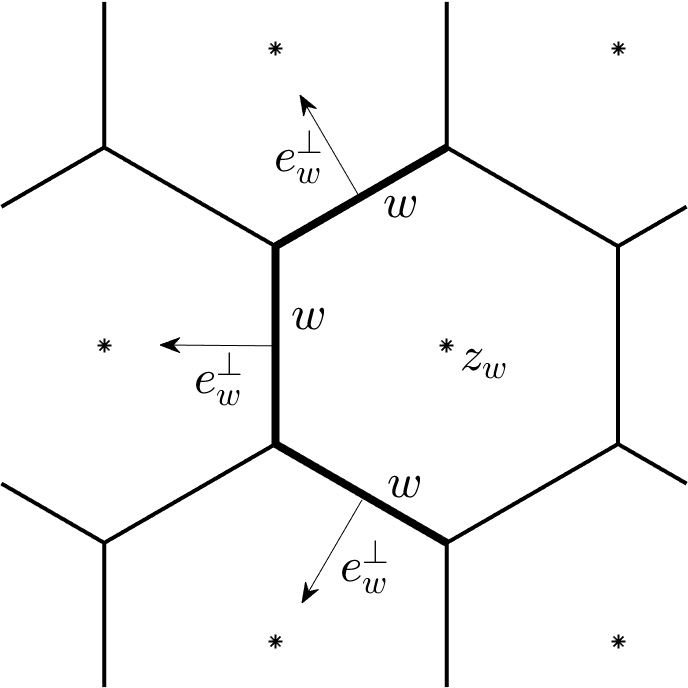
\includegraphics{FigConvLPHexag2.png}}
\end{subfigure}
\hfill
\begin{subfigure}
{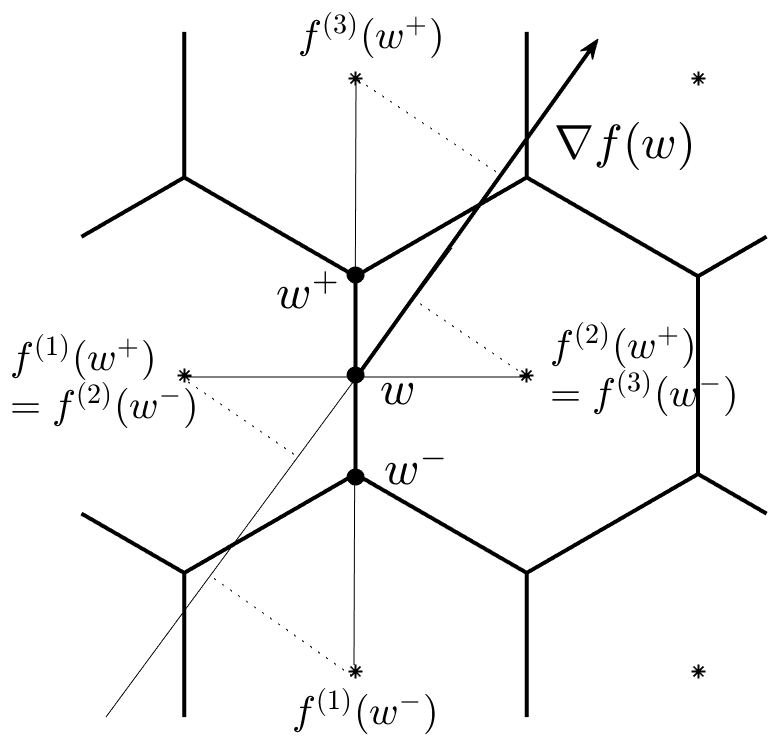
\includegraphics{FigConvLTCHexag2.png}}
\end{subfigure}
\caption{Left: Each edge $w$ is the boundary between two neighbouring hexagons, and we denote by $z_w$ the center of the right-most hexagon. Right: A vertical edge $w$, and its two associated vertices $w^+$ and $w^-$. Given the gradient $\nabla f(w)$, one can find the ordered values of $f$.}\label{FigConvLPHexag2:fig}
\end{figure}


Let $w\in\calE_\eps$ be an edge, that is the boundary between two neighbouring hexagons, and let $z_w$ be the center of the right-most hexagon (i.e. among the two hexagon centers, $z_w$ is the one that has the largest first coordinate). The center of the other hexagon is then $z_w+\eps\sqrt{3} e_w^\perp$, where $e_w$ is the unit length vector oriented as the edge $w$, and $e_w^\perp$ is its $\frac{\pi}{2}$-rotation. See also Figure~\ref{FigConvLPHexag2:fig} left. Then
\begin{align*}
f^+(w) - f^-(w) & = \left| f\left(z_w+\eps\sqrt{3} e_w^\perp\right) - f(z_w)\right|
\\
& = \eps\sqrt{3} \left|\left\langle \nabla f(z_w),e_w^\perp\right\rangle \right| + r_1(z_w,\eps),
\end{align*}
where $|r_1(z_w,\eps)|\leq \tfrac{3}{2}\eps^2 \|D^2 f\|_\infty$. Now, each center $z\in\calC_\eps$ is the $z_w$ of three different $w$, with respective normal orientation $e_w^\perp$ equal to $e_{2\pi/3}$, $e_\pi=-e_0$ and $e_{4\pi/3}=-e_{\pi/3}$. Therefore, we can rewrite
\begin{multline*}
\LP_{f_\eps}(U_\eps) \\
\begin{aligned}
& = \eps \sum_{w\,\in\,\calE_\eps\,\cap\,U_\eps} \left(
\eps\sqrt{3} \left|\left\langle \nabla f(z_w),e_w^\perp\right\rangle \right| + r_1(z_w,\eps) \right) \\
& = \eps^2 \sqrt{3} \sum_{z\,\in\,\calC_\eps\,\cap\,U} \left(\left|\left\langle \nabla f(z),e_0 \right\rangle\right| + \left|\left\langle \nabla f(z),e_{\pi/3} \right\rangle \right| +\left|\left\langle \nabla f(z),e_{2\pi/3} \right\rangle\right|\right) + r_2(\eps),
\end{aligned}
\end{multline*}
with $|r_2(\eps)|\le C\eps \left({\calL}(U) \|D^2 f\|_\infty +{\calH}^1(\partial U)\|\nabla f\|_\infty\right)$, using the fact that $|\calC_\eps\cap U|\linebreak\le C {\calL}(U)
\eps^{-2}$. Then, since the area of each hexagon $\calD(z,\eps)$ is equal to $a_\eps=\frac{3\sqrt{3}}{2}\eps^2$, by Proposition~\ref{approx:prop}, we finally get
\begin{multline*}
\LP_{f_\eps}(U_\eps)\\
\begin{aligned}
& = \frac{2}{3} \eps^2 \frac{3\sqrt{3}}{2} \sum_{z\,\in\,\calC_\eps\,\cap\,U} \left(\left|\left\langle \nabla f(z),e_0 \right\rangle \right| + \left|\left\langle \nabla f(z),e_{\pi/3} \right\rangle\right| +\left|\left\langle \nabla f(z),e_{2\pi/3} \right\rangle\right|\right) + r_2(\eps) \\
& =
\frac{2}{3} \int_U \left(\left|\left\langle
\nabla f(x),e_0\right\rangle\right| +\left|\left\langle \nabla f(x),e_{\pi/3}\right\rangle\right| +\left|\left\langle
\nabla f(x),e_{2\pi/3}\right\rangle\right| \right) \, dx + r_3(\eps),
\end{aligned}
\end{multline*}
with $|r_3(\eps)|\le \eps C_{_{\LP}}^{^{\Hex}}(f,U),$ where
\[
C_{_{\LP}}^{^{\Hex}}(f,U)\le C \left({\calL}(U) \left\|D^2 f\right\|_\infty +{\calH}^1(\partial U)\|\nabla f\|_\infty\right).
\] 
This ends the proof for the level perimeter integral.

%\bigskip

The proof for $\LTC$ also relies on Taylor formulas but now of order 2 instead of 1 and needs a clever grouping of vertices (see Figure~\ref{FigConvLPHexag2:fig} right). The details are postponed to Appendix~\ref{app:limit-deter:th}.
\end{proof}

\subsection{Limit as the square's size \texorpdfstring{$\eps$}{eps} goes to \texorpdfstring{$0$}{0}}

Again, let $U=(0,T)^2$ be a fixed domain. Let $\eps_0>0$, and let us now consider a tiling with squares of size $\eps \in (0,\eps_0]$. Let $f$ be a $C^2$ function defined on $U^{\eps_0}$. We then consider a discretized version $f_\eps\in \PC^{\Sq}_\eps(U^{\eps})$ of $f$ defined by
\begin{equation}\label{disc:sq}
\text{ for a.e. } x\in U^{\eps}, \quad f_\varepsilon(x) =\sum_{z\,\in\,\calC_\eps\,\cap\,U^{\eps}} f(z)
\ind_{\calD(z,\,\eps)}(x),
\end{equation}
where the $\calD(z,\eps)$ are the square tiles, and the boundary conditions are defined as in Section~\ref{LPLTCSq:subsec}. The formulas for $\LP_{f_\eps}(U_\eps)$ and $\LTC_{f_\eps}(U_\eps)$ were given in Proposition~\ref{level-int-discr-square:prop}. We are interested in their limits as $\eps$ goes to $0$, and the links with $\LP_f (U)$ (Equation~\eqref{LPUfsmooth:eq}) and $\LTC_f (U)$ (Equation~\eqref{LTCUfsmooth:eq}).

We first define
\begin{align}
\tLP_{f}^{^{\Sq}}(U) &= \int_U \left(\left|\left\langle
\nabla f(x),e_0\right\rangle\right| +\left|\left\langle \nabla f(x),e_{\pi/2}\right\rangle\right| \right) \, dx\label{LPSq}\\
\intertext{and}
\tLTC_{f}^{^{\Sq}}(U) &= \frac{\pi}{2}\int_U \partial_{12}f(x) \left[\ind_{\nabla\,f(x)\,\in\,Q_+}-\ind_{\nabla\,f(x)\,\in\,Q_-}\right] \, dx,\label{LTCSq}
\end{align}

where here $Q_+=\{z=(z_1,z_2)\in\R^2; z_1z_2>0\}$ and $Q_-=\{z=(z_1,z_2)\in\R^2; z_1z_2<0\}$.



\begin{theo}\label{limit-deter-sq:th}
Let $f$ be a function defined on $U$ and assume that $f$ is $C^2$ on $U^{\eps_0}$ with $\|\nabla f\|_\infty:=\max_{U^{\eps_0}}\|\nabla f\|<+\infty$ and $ \|D^2 f\|_\infty:=\max_{U^{\eps_0}}\|D^2 f\|<+\infty$. For $\eps\in (0,\eps_0]$, let $f_\eps$ be the square discretized version of $f$ on $U^{\eps}$. Then,
\[
\left| \LP_{f_\eps}(U_\eps) - \tLP^{^{\Sq}}_{f}(U) \right| \leq
\eps C_{_{\LP}}^{^{\Sq}}(f,U) \,.
\]
where
\[
C_{_{\LP}}^{^{\Sq}}(f,U)\le C \left({\calL}(U)+{\mathcal
H}^1(\partial U)\right)\left(\|\nabla f\|_\infty+\left\|D^2
f\right\|_\infty\right),
\]
$C$ being a numerical constant independent of everything.

If moreover $f$ is $C^3$ on $U^{\eps_0}$ with $\|D^3 f\|_\infty:=\max_{U^{\eps_0}}\|D^3 f\|<+\infty$, let us introduce the set
\[
{\calU}_{\eps}(f,U) =\left\{ x\in U \, ; \,
\left|\partial_1f(x)\right| < \eps \left\|D^2 f\right\|_\infty \; \text{ or } \;
\left|\partial_2 f(x)\right| < \eps \left\|D^2 f\right\|_\infty \right\}.
\]

Then, there exists a constant $C_{_{\LTC}}^{^{\Sq}}(f,U)$ such that for $\dd \in\{4,6,8\}$,
\begin{align*}
\left|\LTC^{\dd}_{f_\eps}(U_\eps)-\tLTC_{f}^{\Sq}(U)\right| &\le
\eps C_{_{\LTC}}^{^{\Sq}}(f,U)\, + C \left\|D^2 f\right\|_\infty {\calL}\left(\calU_{3\eps}(f,U)\right),
\\
\intertext{where}
C_{_{\LTC}}^{^{\Sq}}(f,U) &\le C\left({\calL}(U)+{\calH}^1(\partial U)\right)\left(\left\|D^2f\right\|_\infty+\left\|D^3f\right\|_\infty\right).
\end{align*}
\end{theo}

\begin{figure}[!htbp]
%\begin{center}
\centering
\hfill
%[width=5cm]
\begin{subfigure}
{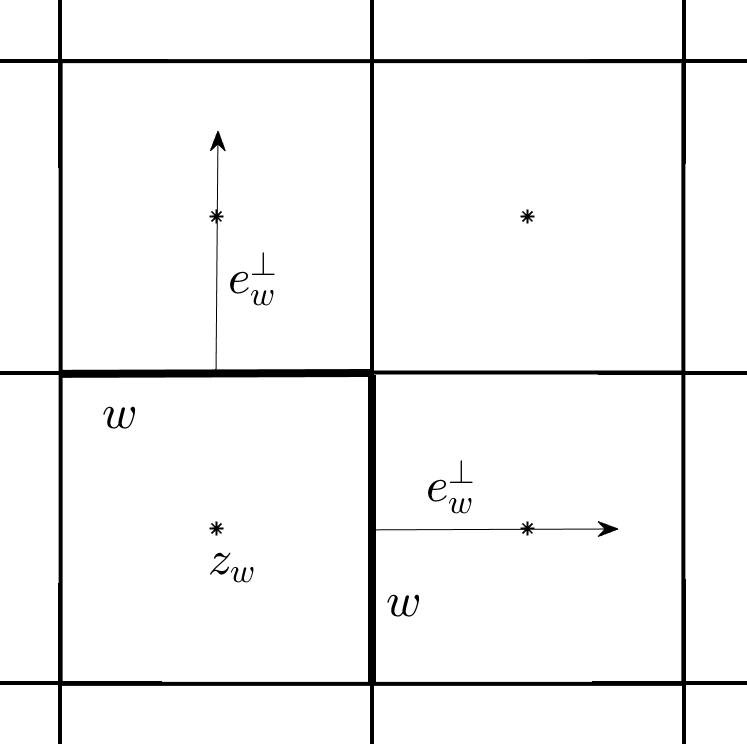
\includegraphics[scale=1.05]{FigConvLPSquare2.png}}
\end{subfigure}
\hfill
\begin{subfigure}
{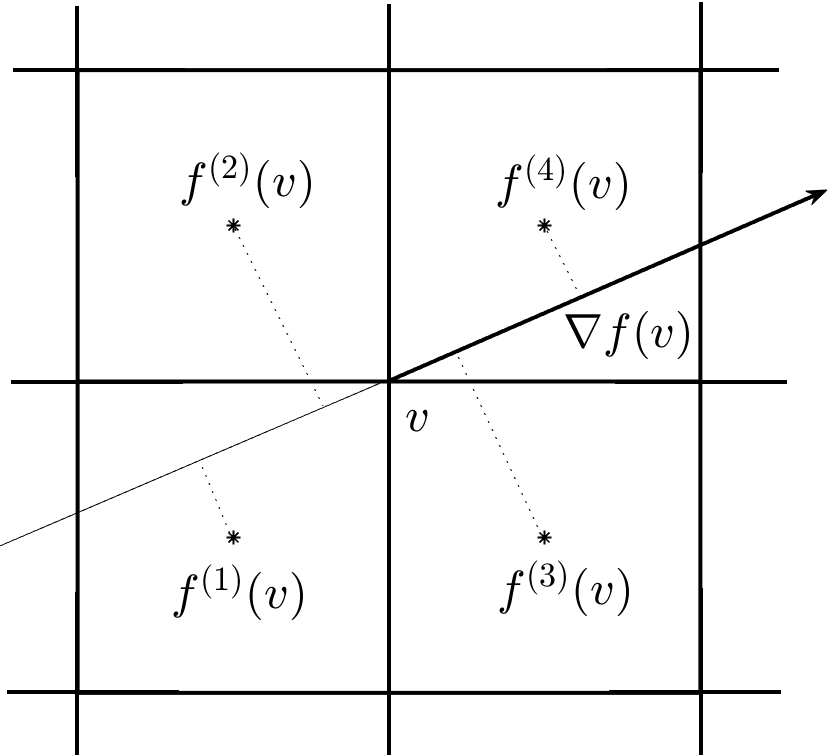
\includegraphics[scale=1.05]{FigConvLTCSquare2.png}}
\end{subfigure}
%\end{center}
\caption{Left: Each edge $w$ is the boundary between two neighbouring squares, and we denote by $z_w$ the center of the left-most (if the edge is vertical) or bottom-most (if the edge is horizontal) square. Right: A vertex $v$, and its four associated centers. Given the gradient $\nabla f(v)$, one can find the ordered values of $f$.}\label{FigConvLPSquare2:fig}
\end{figure}


\begin{proof}
Let us consider the level perimeter integral of $f_\eps$, as $\eps$ goes to $0$, with $f_\eps$ the square discretized version of a $C^2$ function $f$ defined on $U^{\eps_0}$. The computations here will be very similar to the ones in the hexagonal case. We have, by Proposition~\ref{level-int-discr-square:prop}, that
\[
\LP_{f_\eps}(U) = \eps \sum_{w\,\in\,\calE_\eps\,\cap\,U}\left[f^+(w) - f^-(w)\right].
\]

Let $w\in\calE_\eps$ be an edge, that is the boundary between two neighbouring squares, and let $z_w$ be the center of the left-most (if the edge is vertical), or bottom-most (if the edge is horizontal) square. The center of the other square is then $z_w+\eps e_w^\perp$. See Figure~\ref{FigConvLPSquare2:fig} left. Then
\begin{align*}
f^+(w) - f^-(w) & = \left| f\left(z_w+\eps e_w^\perp\right) - f(z_w)\right|
\\
& = \eps \left|\left\langle \nabla f(z_w),e_w^\perp\right\rangle\right| + r_1(z_w,\eps),
\end{align*}
where $|r_1(z_w,\eps)|\leq \eps^2 \|D^2f\|_\infty$, by Taylor formula. Now, each center $z\in\calC_\eps$ is the $z_w$ of two different $w$, with respective normal orientation $e_w^\perp$ equal to $e_{0}$ and $e_{\pi/2}$. Therefore, we can rewrite
\begin{align*}
\LP_{f_\eps}(U_\eps) & = \eps^2 \sum_{w\,\in\,\calE_\eps\,\cap\,U_\eps} \left(\left|\left\langle \nabla f(z_w),e_w^\perp\right\rangle\right| + r_1(z_w,\eps) \right) \\
& = \eps^2 \sum_{z\,\in\,\calC_\eps\,\cap U_\eps} \left(\left|\left\langle \nabla f(z),e_0\right\rangle\right| +\left|\left\langle \nabla f(z),e_{\pi/2}\right\rangle\right|\right) + r_2(\eps),
\end{align*}
with $|r_2(\eps)|\le C\eps \left({\calL}(U) \|D^2 f\|_\infty +{\calH}^1(\partial U)\|\nabla f\|_\infty\right)$, using the fact that $|\calC_\eps \cap U|\linebreak\le C {\calL}(U)
\eps^{-2}$. Then, since the area of each square $\calD(z,\eps)$ is equal to $a_\eps=\eps^2$,\linebreak by Proposition~\ref{approx:prop}, we finally get
\begin{align*}
\LP_{f_\eps}(U_\eps) & = \eps^2 \sum_{z\,\in\,\calC_\eps\,\cap\,U_\eps} \left(\left|\left\langle \nabla f(z),e_0 \right\rangle\right| +\left|\left\langle \nabla f(z),e_{\pi/2} \right\rangle \right||\right) + r_2(\eps) \\
& = \int_U \left(\left|\left\langle
\nabla f(x),e_0\right\rangle\right| +\left|\left\langle \nabla f(x),e_{\pi/2}\right\rangle\right|
\right) \, dx + r_3(\eps),
\end{align*}
with $|r_3(\eps)|\le \eps C_{_{\LP}}^{^{\Sq}}(f,U),$ where $ C_{_{\LP}}^{^{\Sq}}(f,U)\le C \left({\calL}(U) \|D^2 f\|_\infty +{\calH}^1(\partial U)\|\nabla f\|_\infty\right)$. This ends the proof for the level perimeter integral.


%\bigskip
The proof for $\LTC$ is similar but more technical, and it is postponed to Appendix~\ref{app:limit-deter-sq:th}.
\end{proof}



\subsection{Discretizing a smooth random field}

In this section, we will see what happens to the mean level perimeter integral and to the mean level total curvature integral of a discretized smooth stationary random field, in both the hexagonal tiling and the square tiling cases. Roughly speaking, we will see that the perimeter is always biased, whereas the total curvature is not, under an additional isotropy assumption. 


In all this section, as previously, we consider a fixed domain $U=(0,T)^2$.



\begin{prop}\label{cvgce:LP}
Let $X$ be a stationary $C^2$ random field on $\R^2$ such that \[
\|\nabla X\|_\infty=\underset{U^{\eps_0}}{\max}\|\nabla X\|\text{ and }\left\|D^2 X\right\|_\infty=\underset{U^{\eps_0}}{\max}\left\|D^2 X\right\|
\]
have finite expectations for some $\eps_0>0$. Then $\LP_X(U), \tLP^{^{\Hex}}_{X}(U)$ and $\tLP^{^{\Sq}}_{X}(U)$ are in $L^1(\Omega)$.


Let us consider the discretization $X_\eps \in \PC_\eps^{\Hex}(U_\eps)$ as in~\eqref{disc:hexa}, respectively $X_\eps \in \PC_\eps^{\Sq}(U_\eps)$ as in~\eqref{disc:sq}. Then $\LP_{X_\eps}(U_\eps)$ converges to $\tLP^{^{\Hex}}_{X}(U)$, respectively to $\tLP^{^{\Sq}}_{X}(U)$, in $L^1(\Omega)$, as $\eps$ goes to $0$.


Moreover,
\begin{align*}
\frac{2\sqrt{3}}{3} \E(\LP_{X}(U)) &\leq
\E\left(\tLP^{^{\Hex}}_{X}(U)\right) \leq \frac{4}{3} \E\left(\LP_{X}(U)\right),
\\
\intertext{respectively}
\E(\LP_{X}(U)) &\leq \E\left(\tLP^{^{\Sq}}_{X}(U)\right) \leq \sqrt{2} \E\left(\LP_{X}(U)\right).
\end{align*}
Under the additional assumption that $X$ is isotropic we have
\[
\E\left(\tLP^{^{\Hex}}_{X}(U)\right) = \E\left(\tLP^{^{\Sq}}_{X}(U)\right) =
\frac{4}{\pi} \E\left(\LP_{X}(U)\right).
\]
\end{prop}

To give some hints on the numerical values: $\tfrac{2\sqrt{3}}{3}\simeq 1.15$, $\tfrac{4}{3} \simeq 1.33$, $\sqrt{2} \simeq 1.41$ and $\tfrac{4}{\pi} \simeq 1.27$. This shows that, whatever the field, whatever the smallness of the hexagons, there is always a bias when approximating the level perimeter integral of the field $X$ by the one of its discretized version on an hexagonal tiling. There is also a bias on a square tiling, except if the smooth field $X$ has a gradient that is everywhere aligned with $e_0$ or $e_{\frac{\pi}{2}}$. The strongest bias is obtained when the gradient is everywhere aligned with the diagonal directions $e_{\frac{\pi}{4}}$ or $e_{-\frac{\pi}{4}}$. These last remarks are consequences of the proofs below.

\begin{proof}
Under our assumptions it is clear that $\LP_{X_\eps}(U_\eps), \LP_X(U), \tLP^{^{\Hex}}_{X}(U)$ and $\tLP^{^{\Sq}}_{X}(U)$ are in $L^1(\Omega)$. Moreover we also have that $C_{\LP}^{^{\Hex}}(X,U)$ and $C_{\LP}^{^{\Sq}}(X,U)$ are in $L^1(\Omega)$ so that the convergence results hold taking expectation from Theorems~\ref{limit-deter:th} and~\ref{limit-deter-sq:th}. According to the beginning of Section~\ref{DoSF:sec}, by Fubini theorem and the stationarity of $X$, we have
\[
\E\left(\LP_{X}(U)\right) = \int_U \E \left(\left\|\nabla X(x)\right\|\right) \, dx = \calL(U)
\E \left(\left\|\nabla X(0)\right\|\right),
\]
whereas we have
\begin{align*}
\E\left(\tLP^{^{\Hex}}_{X}(U)\right) &= \frac{2}{3} \calL(U) \E \left(
\left|\left\langle \nabla X(0), e_0\right\rangle\right| + \left|\left\langle \nabla X(0), e_{\frac{\pi}{3}}\right\rangle\right| +\left|\left\langle \nabla X(0),
e_{\frac{2\pi}{3}}\right\rangle\right|\right)
\\
\text{ and } \quad \E\left(\tLP^{^{\Sq}}_{X}(U)\right) &= {\calL}(U)
\E \left(\left(\left|\left\langle \nabla X(0), e_0\right\rangle\right| +\left|\left\langle \nabla
X(0), e_{\frac{\pi}{2}}\right\rangle\right|\right)\right).
\end{align*}
Now, a simple computation shows that for any $\theta\in\R$, we have
\[
\sqrt{3} \leq |\cos\theta| + \left|\cos\left(\theta-\frac{\pi}{3}\right)\right| +
\left|\cos\left(\theta-\frac{2\pi}{3}\right)\right| \leq 2.
\]
Therefore
\[
\frac{2\sqrt{3}}{3} \E\left(\LP_{X}(U)\right) \leq
\E\left(\tLP^{^{\Hex}}_{X}(U)\right) \leq \frac{4}{3} \E\left(\LP_{X}(U)\right).
\]
In the case of a tiling with squares, since for any $\theta\in\R$ we have
\begin{align*}
1 &\leq |\cos\theta| + |\sin\theta| \leq \sqrt{2},
\\
\intertext{we obtain}
\E\left(\LP_{X}(U)\right) &\leq \E\left(\tLP^{^{\Sq}}_{X}(U)\right) \quad\!\leq \sqrt{2} \E\left(\LP_{X}(U)\right).
\end{align*}


When the smooth stationary random field $X$ is moreover isotropic, $\nabla X$ is rotationally invariant and, according to~\cite[Proposition~4.10]{Bilodeau}, its gradient direction $\nabla X(x)/\| \nabla X(x)\|$ is independent from $\| \nabla X(x)\|$ and uniform on $S^1$. Thus we get, for any $\theta\in[0,2\pi)$,
\[
\E\big(\left|\left\langle \nabla X(0), e_\theta\right\rangle\right|\big) = \E\left(
\left\| \nabla X(0) \right\|\right) \int_0^{2\pi}\left|\cos\left(\varphi-\theta\right)\right| \,
\frac{1}{2\pi} d\varphi = \frac{2}{\pi} \E\left(\left\| \nabla X(0)\right\|\right)
.
\]
This shows that in the isotropic case
\[
\E\left(\tLP^{^{\Hex}}_{X}(U)\right) = \E\left(\tLP^{^{\Sq}}_{X}(U)\right) =
\frac{4}{\pi} \E\left(\LP_{X}(U)\right),
\]
and since $\frac{4}{\pi}>1$, there is always a bias.
\end{proof}

\pagebreak
\begin{rema}
Assuming moreover that $\E(\|\nabla X\|_\infty^2)<+\infty$, for any $h:\R\rightarrow
\R$ bounded $C^1$ function with derivative $h'\in C_b(\R)$, and denoting by $H$ a primitive of $h$, then the random field $H\circ X$ will satisfy the assumptions of Proposition~\ref{cvgce:LP}. By linearity this allows us to state the convergence results for $\LP_{X_\eps}(h,U_\eps)$ and obtain in the isotropic case the weak convergence
\[
\E\left(\Per(E_{X_\eps}(t),U_\eps)\right)\rightharpoonup \frac{4}{\pi} \E\left(\Per(E_{X}(t),U)\right),
\]
as remarked in the Gaussian setting of Section~\ref{GaussianDiscret:sec}. This is illustrated on Figure~\ref{StatGaussT100:fig} and it explains why computing perimeters from discrete images is not easy. However, solutions exist to obtain non-biased estimates of the level perimeter integrals from pixelated images, and we propose such a solution in the Appendix~\ref{unbiased:app}. The idea behind the unbiased estimation of the perimeter given in the Appendix~\ref{unbiased:app} in the square tilling framework is to linearly interpolate the function inside each dual square and approximate the boundary of each level set by a polygonal line where now segments are not only horizontal or vertical (as for the discretized function). We show in the Appendix why this linear interpolate provides unbiased estimates of the level perimeter integral. See also Figure~\ref{ExampleSmooth:fig}, where we used a non-Gaussian smooth isotropic shot noise field as considered in~\cite{BD-Geometry-published}.
\end{rema}


%\bigskip

For the level total curvature, things are different: there is no bias. Intuitively this can be explained by the fact that the total curvature is related to the Euler characteristic that counts the number of connected components and the number of holes, and these numbers remain (almost) the same when the function is discretized on very small hexagons or squares.

\begin{prop}\label{cvgce:LTC}
Let $X$ be a stationary $C^3$ random field on $\R^2$ such that \[
\|\nabla X\|_\infty=\underset{U^{\eps_0}}{\max}\|\nabla X\|,\, \left\|D^2 X\right\|_\infty=\underset{U^{\eps_0}}{\max}\left\|D^2 X\right\|\text{ and }\left\|D^3 X\right\|_\infty=\underset{U^{\eps_0}}{\max}\left\|D^3 X\right\|
\]
have finite expectations for some $\eps_0>0$.
Then $\LTC_X(U), \tLTC^{^{\Hex}}_{X}(U)$ and $\tLTC^{^{\Sq}}_{X}(U)$ are in $L^1(\Omega)$.


Let us consider the discretization $X_\eps \in \PC_\eps^{\Hex}(U_\eps)$ as in~\eqref{disc:hexa}, respectively $X_\eps \in \PC_\eps^{\Sq}(U_\eps)$ as in~\eqref{disc:sq}. Assume that $\bbP(\langle \nabla X(0),e_\theta\rangle=0)=0$ for $\theta\in\{\tfrac{\pi}{3},\tfrac{2\pi}{3}\}$, resp. for $\theta\in\{0,\tfrac{\pi}{2}\}$. Then, $\LTC_{X_\eps}(U_\eps)$, resp. $\LTC^{\dd}_{X_\eps}(U_\eps)$ for any $d\in\{4,6,8\}$, converges to $\tLTC^{^{\Hex}}_{X}(U)$ in $L^1(\Omega)$, resp. to $\tLTC^{^{\Sq}}_{X}(U)$, as $\eps$ goes to $0$.


Moreover, under the additional assumption that $X$ is isotropic
\[
\E\left(\tLTC^{^{\Hex}}_{X}(U)\right) =\E\left(\tLTC^{^{\Sq}}_{X}(U)\right) =
\E\left(\LTC_{X}(U)\right).
\]
\end{prop}

\begin{proof}
We begin with the proof of the square tiling
discretization. Under our assumptions it is clear that $\LTC_X(U),
\LTC^{\dd}_{X_\eps}(U_\eps)$ and $\tLTC^{^{\Sq}}_{X}(U)$ are in $L^1(\Omega)$. Moreover we also have $C_{\LTC}^{\Sq}(X,U)$ in $L^1(\Omega)$ and since ${\calL}(\calU_{\eps}(X,U))$ is bounded by ${\calL}(U)$ we can take the expectation in the a.s. inequality stated in Theorem~\ref{limit-deter-sq:th}. Now we have by Fubini theorem and stationarity,
\[
\E\left({\calL}(\calU_{\eps}(X,U))\right)={\calL}(U)\bbP\left(\left|\partial_1 X(0)\right|<\eps \left\|D^2 X\right\|_\infty \text{ or } \left|\partial_2 X(0)\right|<\eps \left\|D^2 X\right\|_\infty \right).
\]
But for $j=1,2$,
\begin{align*}
\bbP\left(\left|\partial_j X(0)\right|<\eps \left\|D^2 X\right\|_\infty\right)&\le \bbP\left(\left|\partial_j X(0)\right|<\eps^{1/2}\right)+ \bbP\left(\left\|D^2 X\right\|_\infty>\eps^{-1/2}\right)\\
&\le \bbP\left(\left|\partial_j X(0)\right|<\eps^{1/2}\right)+\eps^{1/2}\E\left(\left\|D^2 X\right\|_\infty\right)
\end{align*}
by Markov inequality. Since $\lim_{\eps\rightarrow 0}\bbP(|\partial_j X(0)|<\eps^{1/2})=\bbP(\partial_j X(0)=0)=0$ by assumption, we can conclude that ${\calL}(\calU_{\eps}(X,U))$ converges to $0$ in $L^1(\Omega)$ and thus in probability. Hence $\|D^2 X\|_\infty {\calL}(\calU_{\eps}(X,U))$ converges to $0$ in probability and since the variables $\{\|D^2 X\|_\infty {\calL}(\calU_{\eps}(X,U)); \eps\in (0,\eps_0]\}$ are uniformly integrable (because they are uniformly bounded by ${\calL}(U)\|D^2 X\|_\infty$) we also have that $\|D^2 X\|_\infty {\calL}(\calU_{\eps}(X,U))$ converges to $0$ in $L^1(\Omega)$. According to Theorem~\ref{limit-deter-sq:th} this implies that $\LTC^\dd_{X_\eps}(U_\eps)$ converges to $\tLTC^{^{\Sq}}_{X}(U)$ in $L^1(\Omega)$. Moreover by stationarity we obtain
\[
\E\left(\tLTC^{^{\Sq}}_{X}(U)\right)={\calL}(U)\times \frac{\pi}{2}\E\left(\partial_{12}X(0)\left(\ind_{\nabla\,X(0)\,\in\,Q^+}-\ind_{\nabla\, X(0)\,\in\,Q^+}\right)\right).
\]
Now let us assume also that $X$ is isotropic and remark that our assumption implies that $\nabla X(0)\neq 0$ a.s. Hence let us define $\Theta$ as the argument of the gradient $\nabla X(0)$ and write
\[
\E\left(\tLTC^{^{\Sq}}_{X}(U)\right)={\calL}(U)\times \frac{\pi}{2}\E\left(\partial_{12}X(0)g(\Theta)\right),
\]
where $g$ is the $\pi$ periodic function piecewise $C^1$ defined by $g(\theta)=1$ if $\theta\in (0,\pi/2)$, $g(\theta)=-1$ if $\theta\in (\pi/2,\pi)$ and $g(\theta)=0$ if $\theta\in\{0,\frac{\pi}{2}\}$. Then, using the Fourier series of $g$ and the isotropy of $X$, we can show (see the Appendix~\ref{cvLTC:app}) that
\begin{align*}
\E\left(\tLTC^{^{\Sq}}_{X}(U)\right)&=\calL(U)\times
\frac{\pi}{2}\E\left(\partial_{12}X(0)g(\Theta)\right) \\
&=- {\calL}(U) \E\left(\frac{D^2X(0)\cdot \left(\nabla X(0)^\perp,\nabla X(0)^\perp\right)}{\left\|\nabla X(0)\right\|^2}\right)\\
&=\E\left(\LTC_X(U)\right).
\end{align*}

%\medskip

Now let us consider the hexagonal tiling case. The first part follows similarly using Theorem~\ref{limit-deter:th}, once we have remarked that
\begin{multline*}
{\calO}_{\eps}(X,U)\\
\subset \left\{ x\in U ;\left|\left\langle X(x), e_{\pi/3}\right\rangle\right|<3\eps\left\|D^2X\right\|_\infty \text{ or } \left|\left\langle X(x), e_{2\pi/3}\right\rangle\right|<3\eps\left\|D^2X\right\|_\infty\right\}.
\end{multline*}
Then, by stationarity we obtain
\begin{multline*}
\E\left(\tLTC^{^{\Hex}}_{X}(U)\right)\\
={\calL}(U)\times \frac{\pi}{3\sqrt{3}}\E\left(\left[\frac{3}{2}\partial_{22}X(0)
-\frac{1}{2}\partial_{11}X(0)\right]\left(\ind_{\nabla\,X(0)\,\in\,C_1}-2\ind_{\nabla\,X(0)\,\in\,C_0}\right)\right).
\end{multline*}

\pagebreak

Assuming moreover that $X$ is isotropic, again our assumption implies that $\nabla X(0)\neq 0$ a.s. As previously we define $\Theta$ as the argument of the gradient $\nabla X(0)$ and write
\[
\E\left(\tLTC^{^{\Hex}}_{X}(U)\right)=
\calL(U)\times
\frac{\pi}{3\sqrt{3}}\E\left(\left[\frac{3}{2}\partial_{22}X(0)
-\frac{1}{2}\partial_{11}X(0)\right]g(\Theta)\right),
\]
where $g$ is now the $\pi$-periodic function define on $[-\pi/6,5\pi/6]$ by $g=\ind_{(\pi/6,\,5\pi/6)}\linebreak-2\ind_{(-\pi/6,\,\pi/6)}$. Here again, using the Fourier series of $g$ and the isotropy of $X$ (see the technical details in the Appendix~\ref{cvLTC:app}), we can show that
\[
\E\left(\tLTC^{^{\Hex}}_{X}(U)\right) =\E\left(\LTC_X(U)\right).\qedhere
\]
\end{proof}



\begin{figure}[!hbp]
\begin{center}
%\begin{tabular}{ll}
\hfill
\begin{subfigure}
{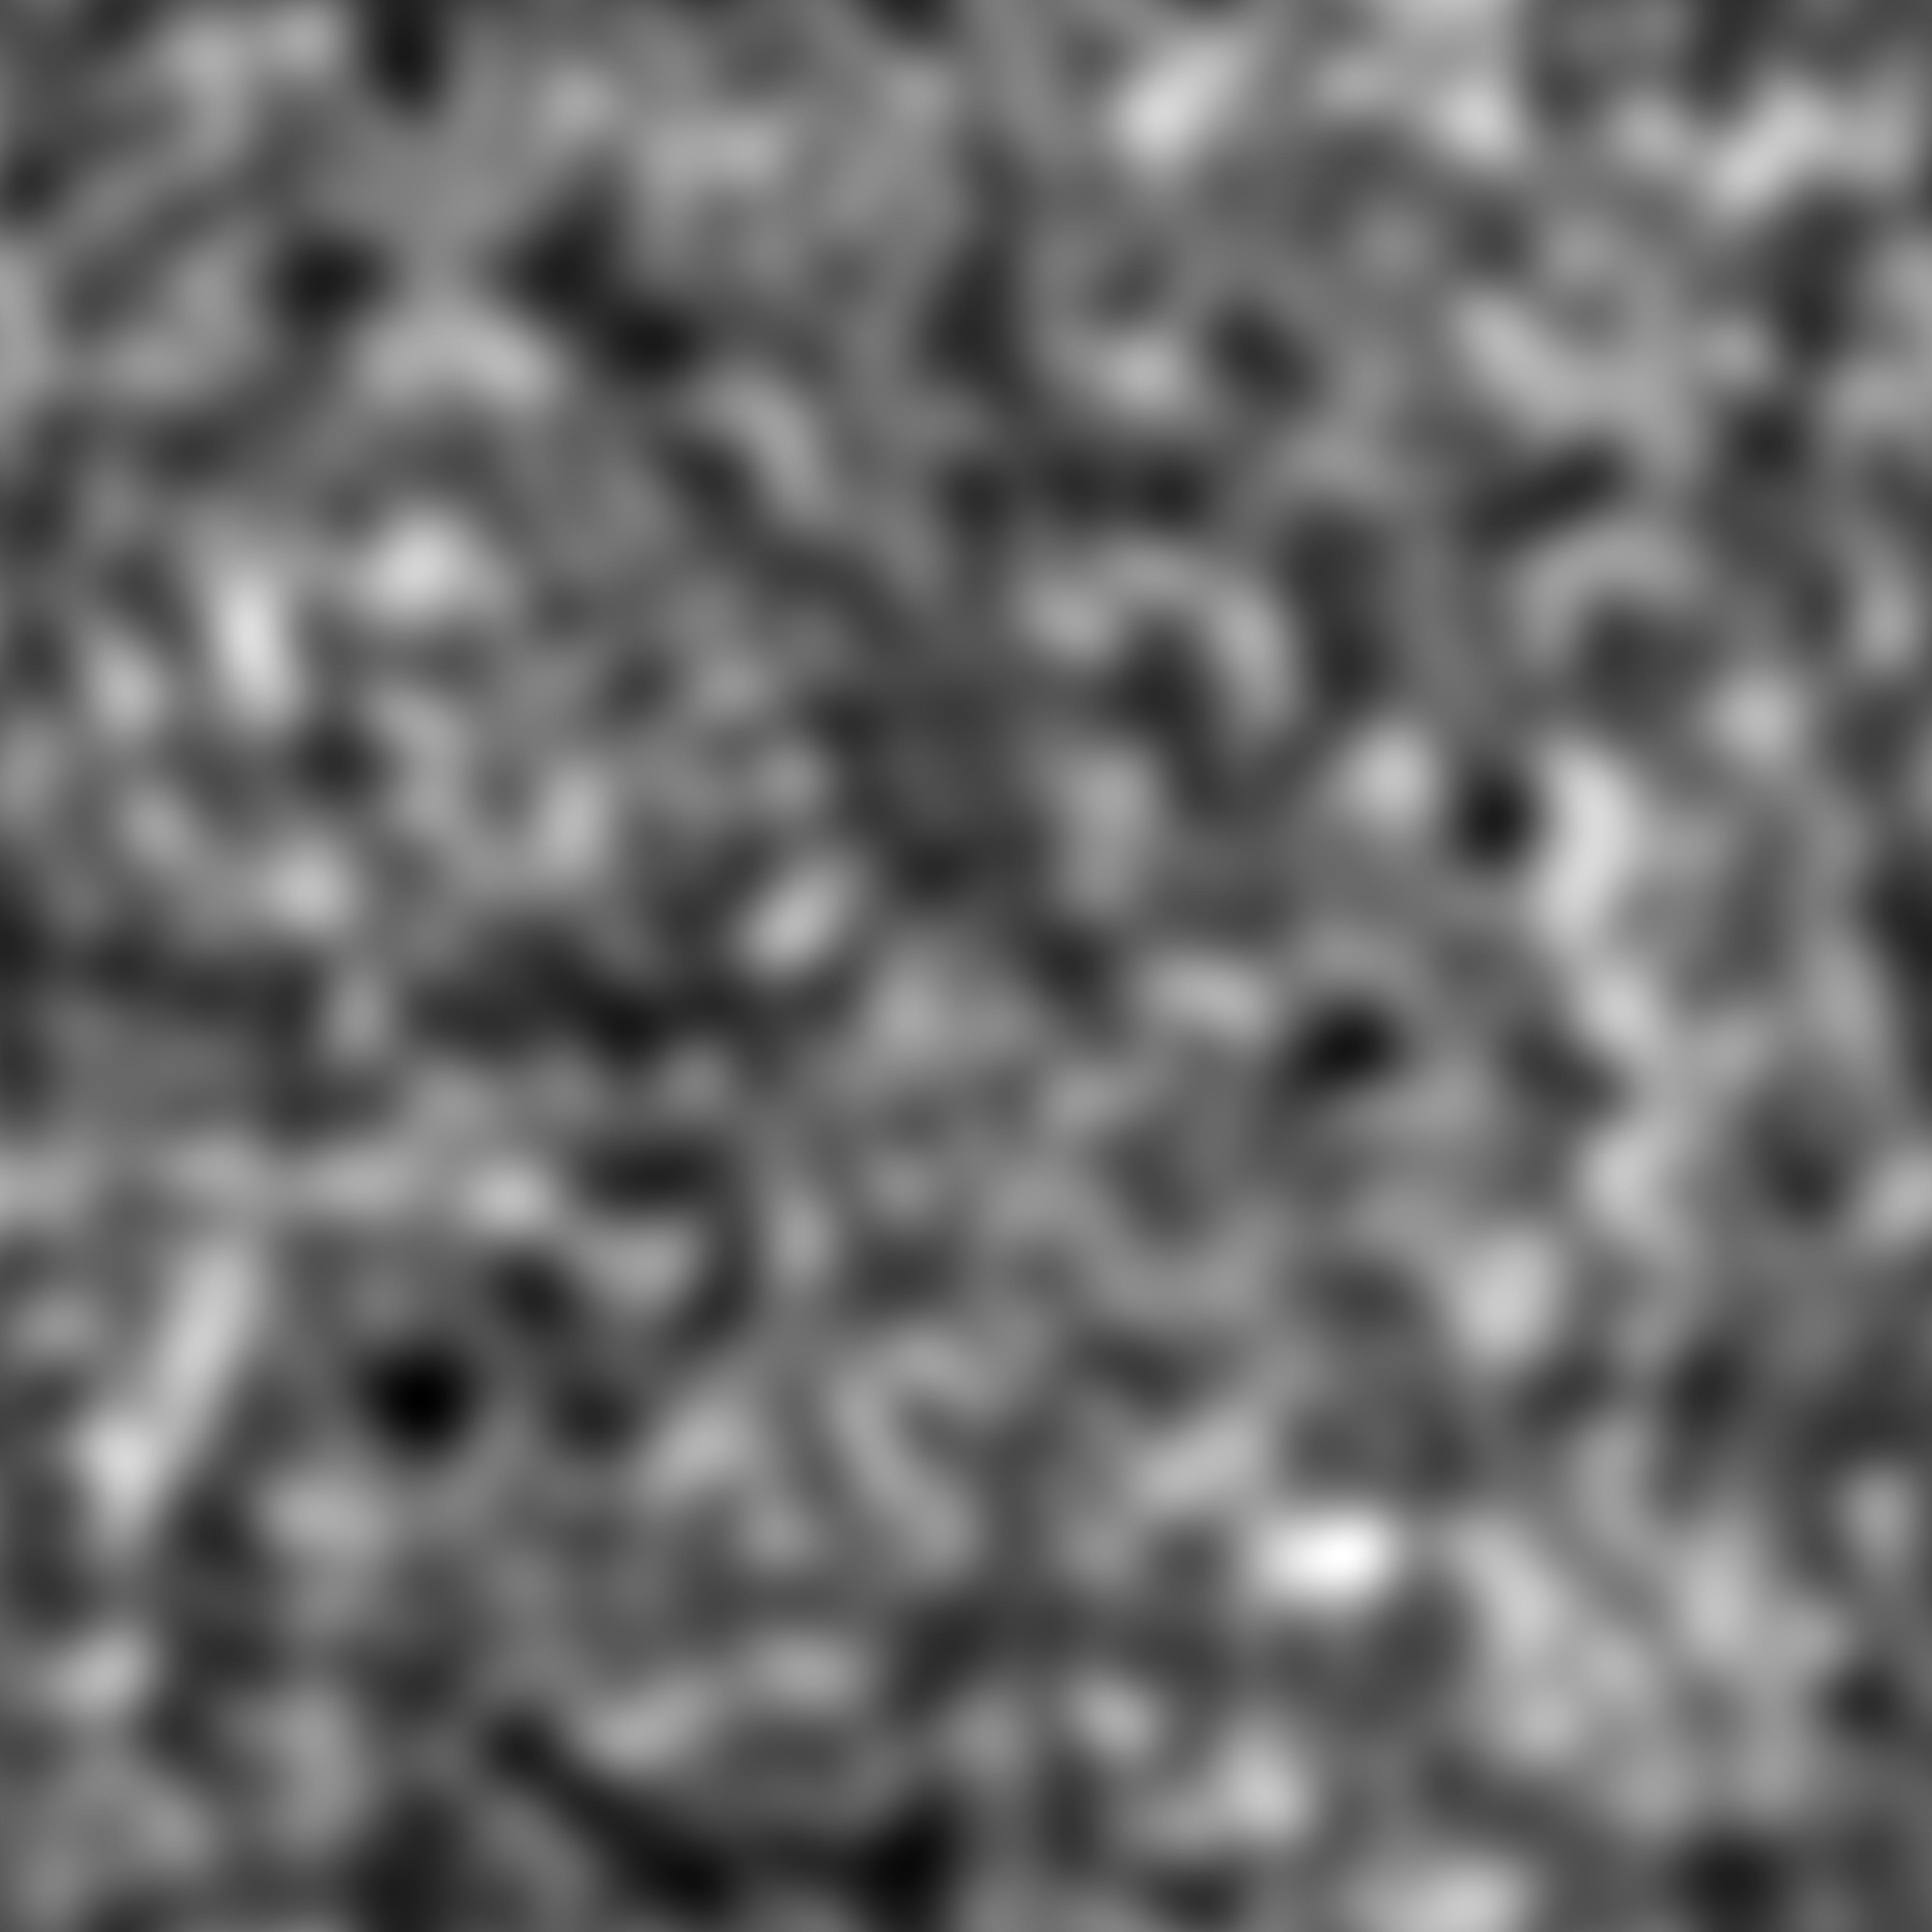
\includegraphics[scale=0.40]{ExampleSmoothImage0.png}}
\end{subfigure}
\hfill
\begin{subfigure}
%[width=5cm]
{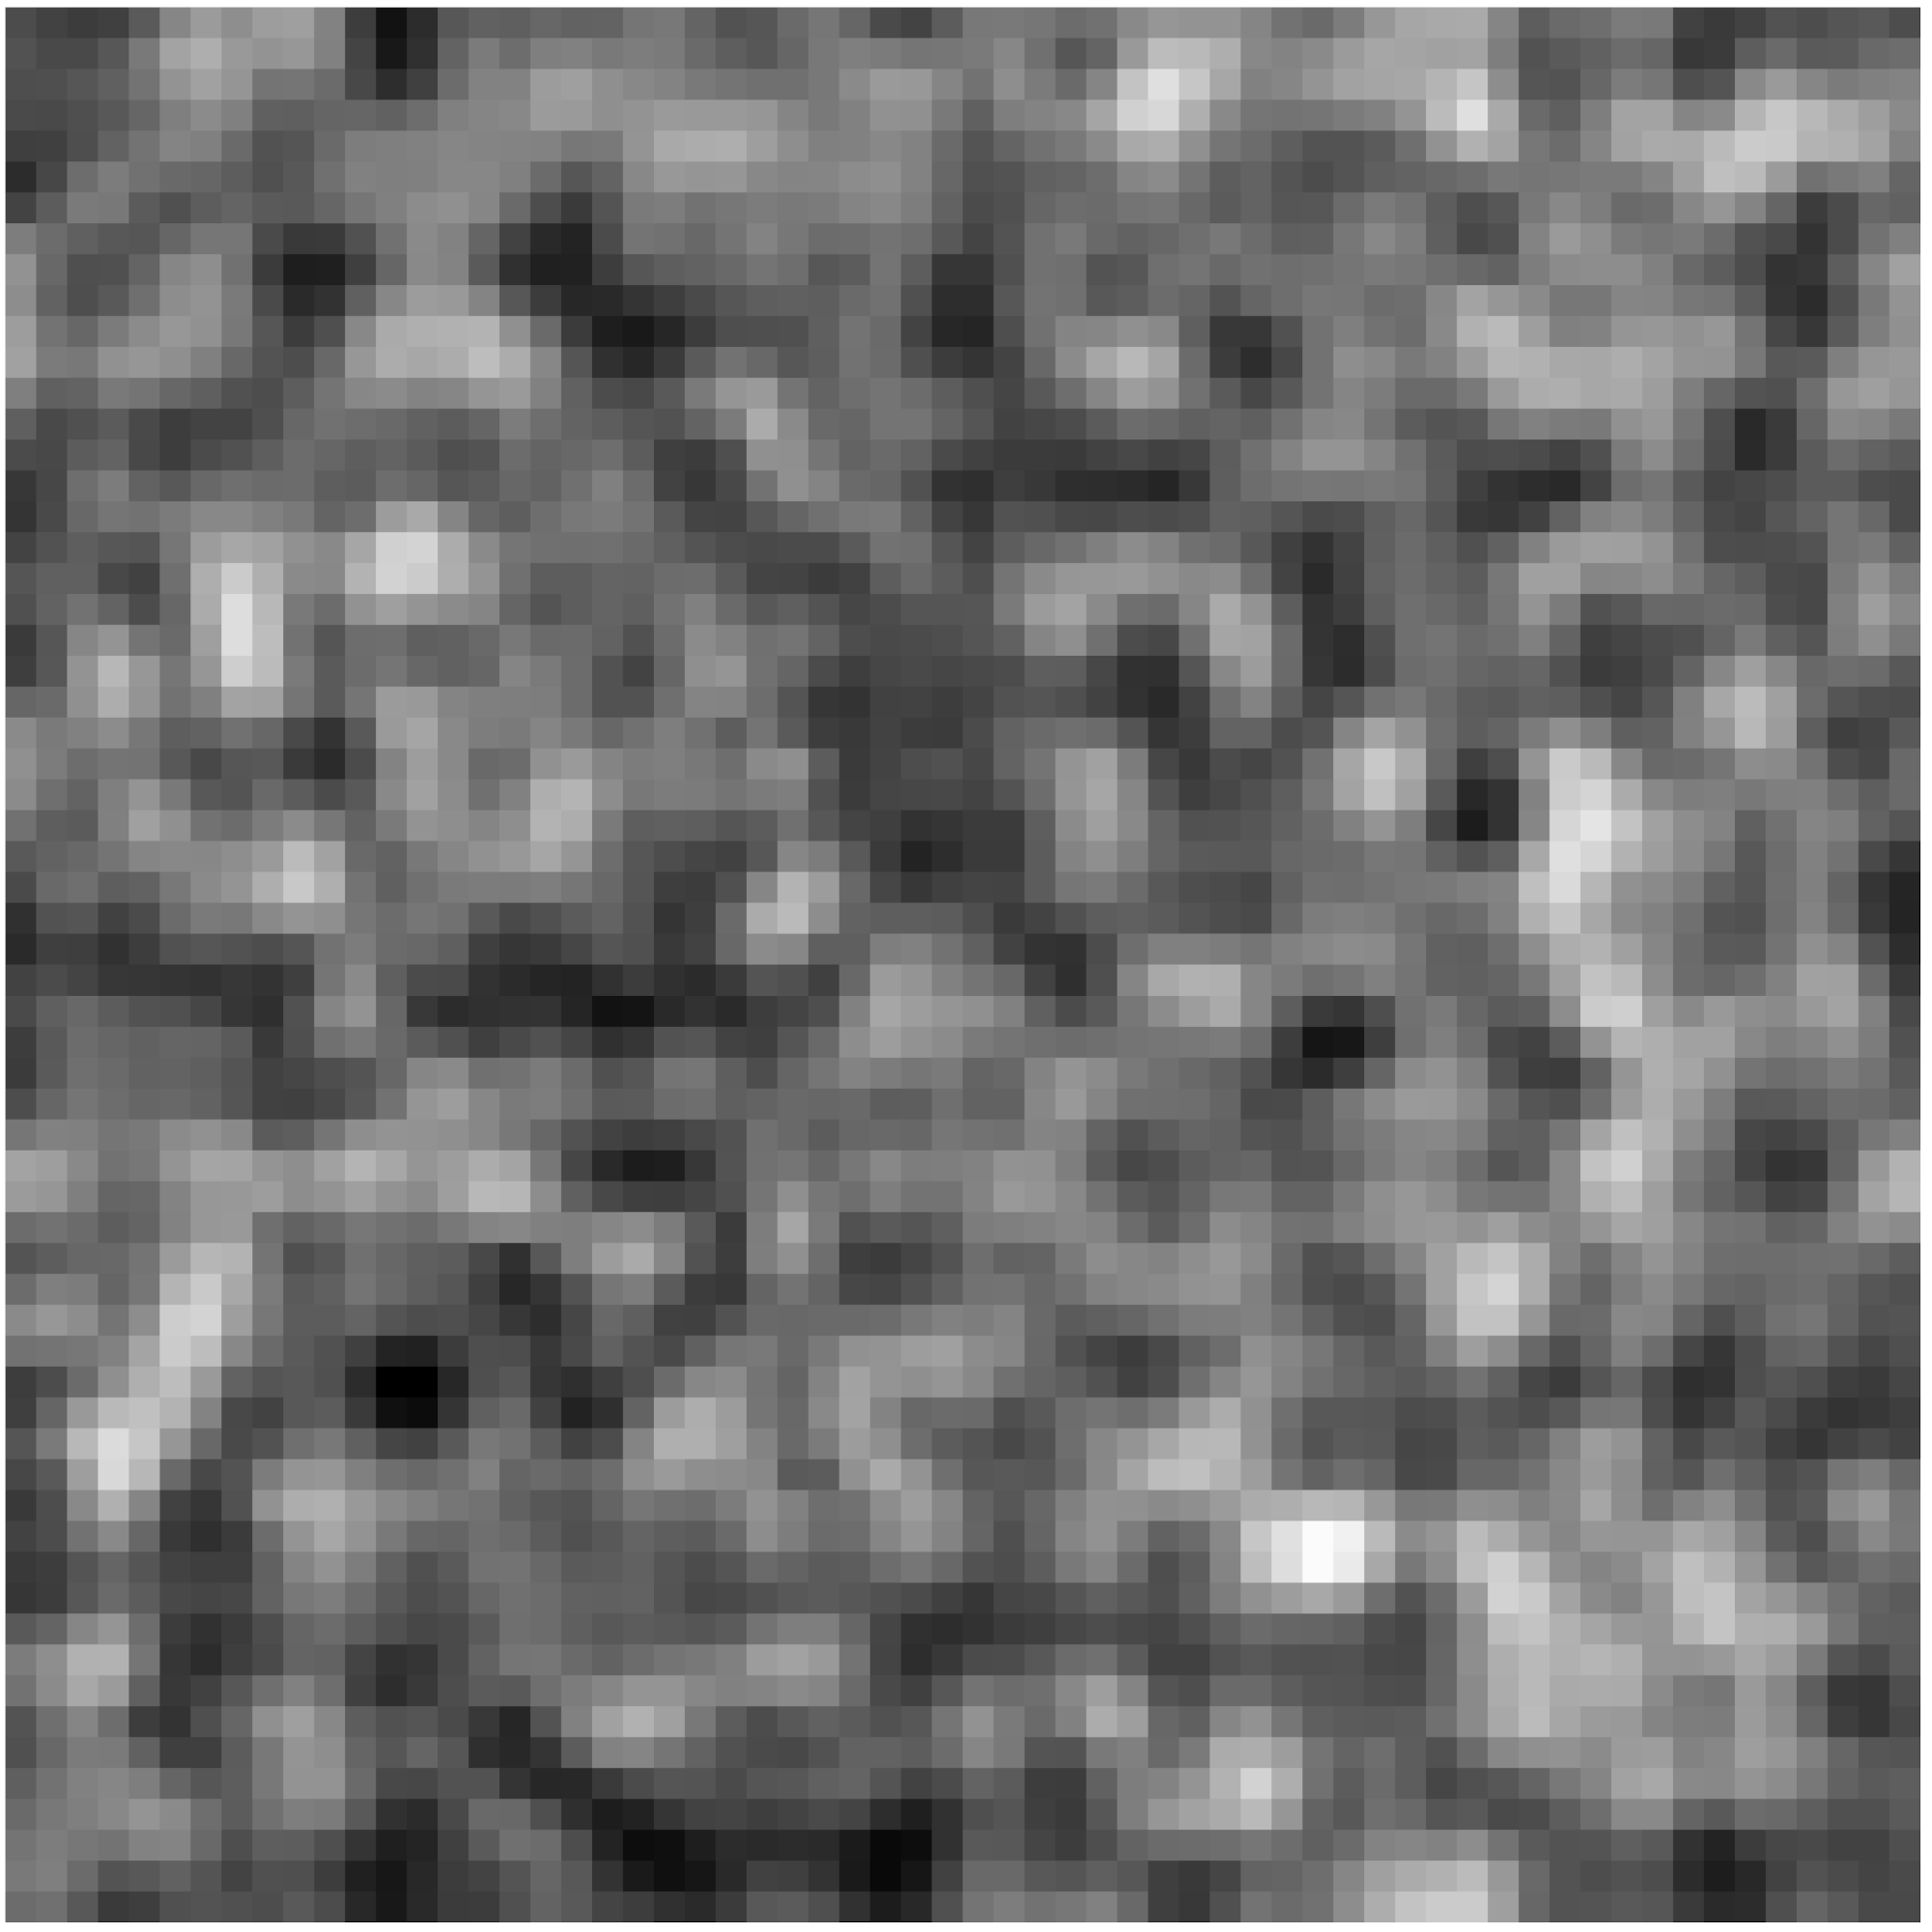
\includegraphics[scale=0.40]{ExampleSmoothImage6.png}}
\end{subfigure}
\\
\begin{subfigure}
{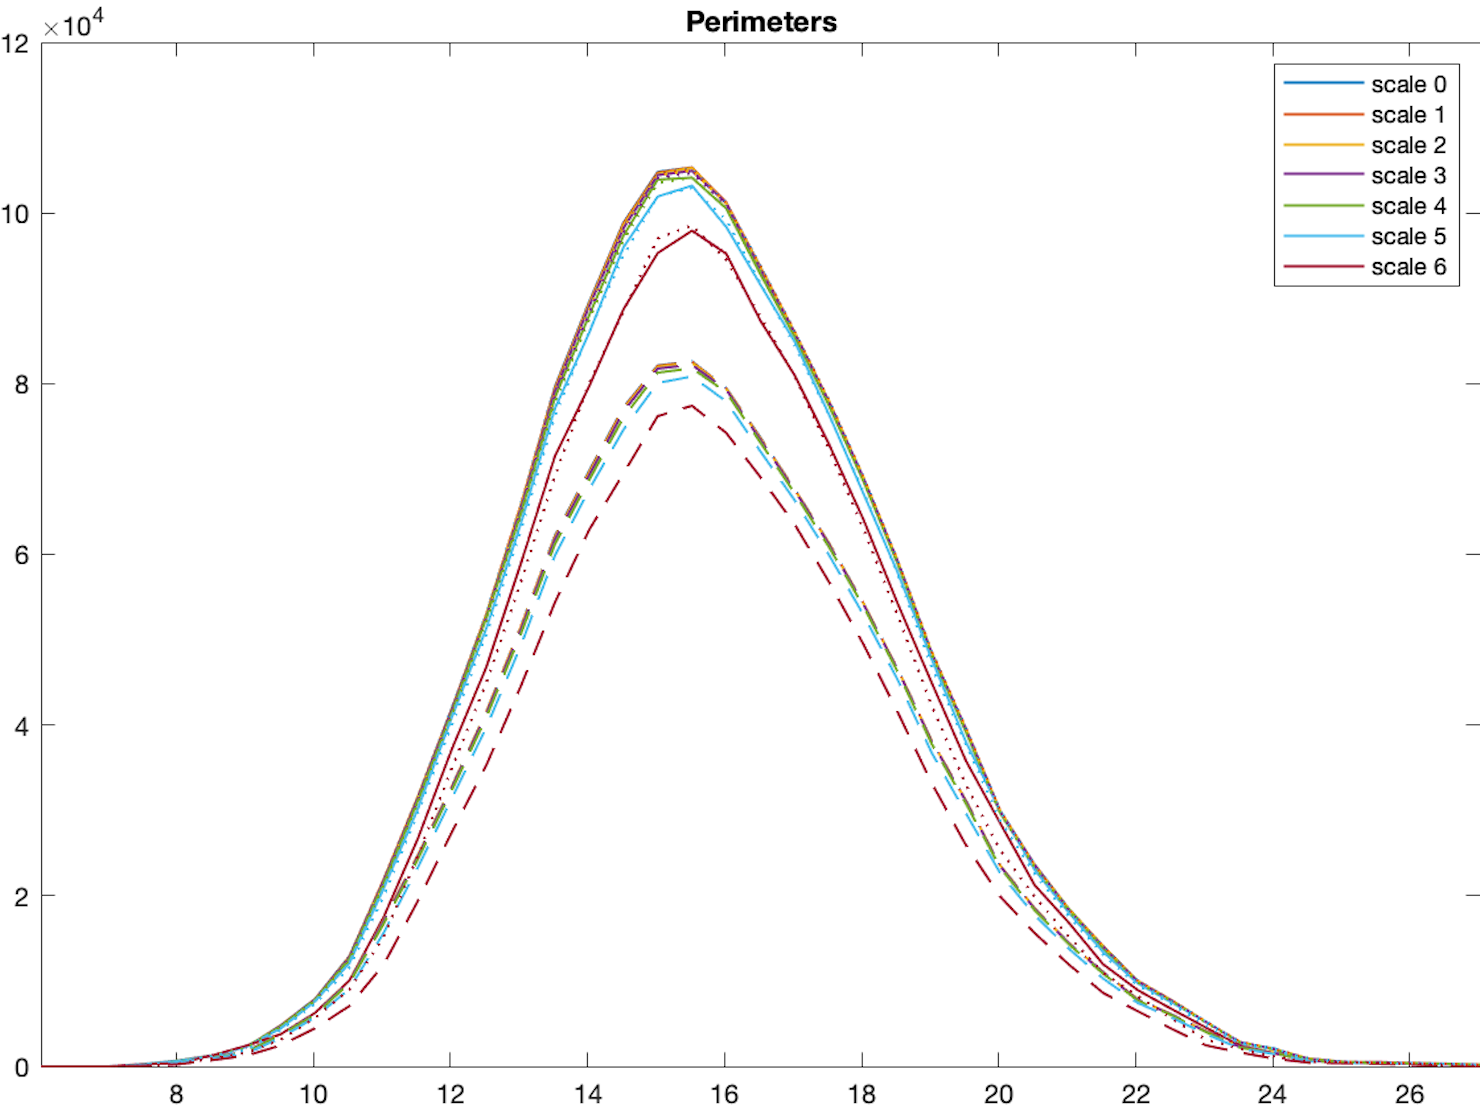
\includegraphics[scale=0.50]{ExampleSmoothPerimeters.png}}
\end{subfigure}
\hspace{10mm}
\begin{subfigure}
{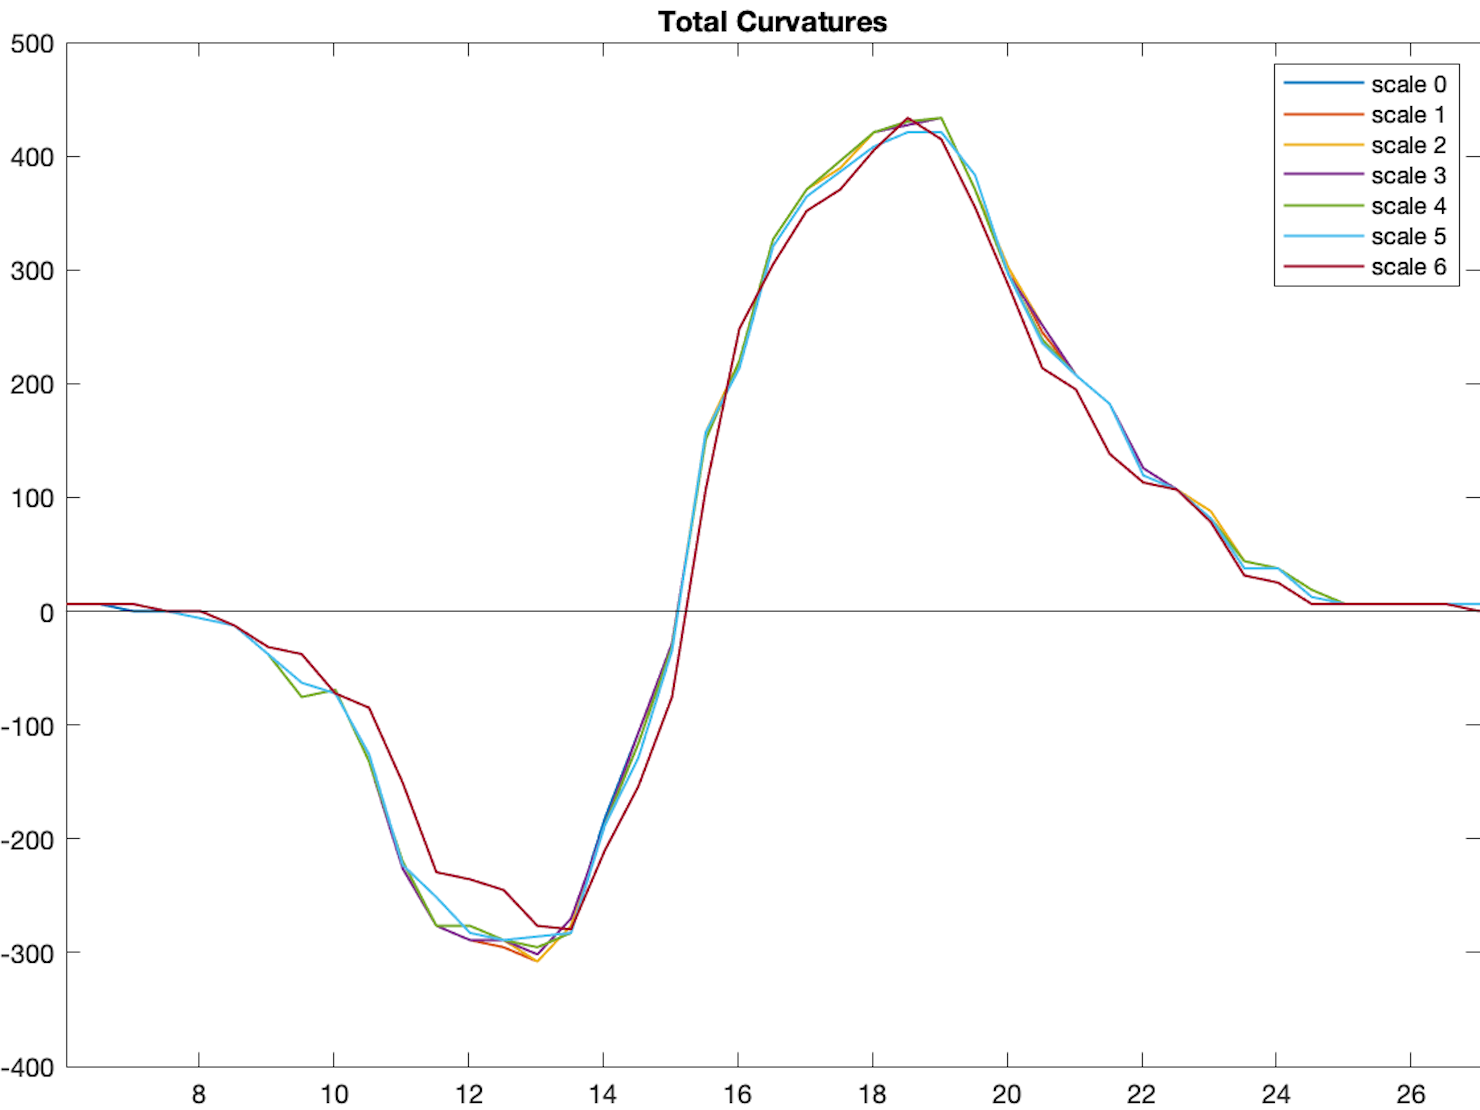
\includegraphics[scale=0.50]{ExampleSmoothCurvatures.png}}
\end{subfigure}
%\end{tabular}
\end{center}
\caption{Top line: on the left, a sample on $(0,1)^2$ of a smooth shot noise random field $X$ with Gaussian kernel~\cite{BD-Geometry-published} on a digital image of size $4000\times 4000$ pixels, i.e. field $X_\eps$ with here $\eps=1/4000$. On the right, same field $X$ but now discretized on a $62\times 62$ pixels grid. It corresponds to a ``scale'' $s=6$, since $62=\lfloor 4000/2^{s} \rfloor$ with $s=6$. Bottom line: on the left, the perimeter of the excursion sets of $X_\eps$ as a function of the level $t$ (in abscissa) - only values of $t$ multiples of $.5$ have been used, hence the plot is a polygonal curve - for different scales $s$ (different colors). The plain curve is the perimeter as defined for discretized fields, the dashed curve is the unbiased perimeter computed as in Appendix~\ref{unbiased:app}, and the dotted curve is $4/\pi$ times the unbiased perimeter. It fits quite well the plain curve, illustrating Proposition~\ref{cvgce:LP}. On the bottom right, the total curvature $\TC^6$ of the excursion sets of $X_\eps$ as a function of the level $t$ (in abscissa) - again, only values of $t$ multiples of $.5$ have been used, hence the plot is a polygonal curve - for different scales $s$ (different colors). As intuitively expected, and except for the coarsest scale $s=6$, whatever the size of the discretization, the values of the total curvature remain almost the same. }\label{ExampleSmooth:fig}
\end{figure}

Let us remark that assuming moreover that $\E(\|\nabla X\|_\infty^3)<+\infty$ and $\E(\|D^2 X\|_\infty^2)\linebreak <+\infty$, for any $h:\R\rightarrow \R$ bounded $C^2$ function with $h'$ and $h''$ bounded, denoting by $H$ a primitive of $h$, the random field $H\circ X$ will also satisfies assumptions of Proposition~\ref{cvgce:LTC} as soon as $\bbP(h(X(0))=0)=0$. By linearity this allows us to state the convergence results for $\LTC^\dd_{X_\eps}(h,U_\eps)$ and obtain in the isotropic case the weak-convergence (according to the set of admissible test functions $h$)
\[
\E\left(\TC^\dd\left(\partial E_{X_\eps}(t)\cap U_\eps\right)\right)\rightharpoonup
\E\left(\TC(\partial E_{X}(t) \cap U)\right),
\]
as remarked in the Gaussian setting. It explains that there is no bias on the level total curvature when discretizing a smooth isotropic stationary random field. This is illustrated on Figure~\ref{StatGaussT100:fig} for a Gaussian field and on Figure~\ref{ExampleSmooth:fig} for a smooth isotropic shot noise field. This last figure also shows the robustness of $\TC$ with respect to the scales of resolution.


%\medskip

\begin{rema}
Let us notice that by the formula for $\LTC_{X_\eps}$ in Proposition~\ref{level-int-discr:prop}, we have in the hexagonal tiling case,
\[
\LTC_{X_\eps}(U_\eps)=\frac{\pi}{3}\sum_{v\,\in\, {\calV}_\eps\,\cap\,U_\eps} \left[X^{(3)}(v)+X^{(1)}(v)-2X^{(2)}(v)\right].
\]
\end{rema}

We see that it involves $X^{(2)}(v)$, that is the median value around $v$. In the square tiling case, there are two median values given by $X^{(2)}(v)$ and $X^{(3)}(v)$. Hence we have here shown an interesting link between median value and curvature since, as $\eps$ goes to $0$, the limit of $\LTC_{X_\eps}(U_\eps)$ is, in expectation, the curvature of the smooth function $X$. This link was already well-known in the field of mathematical image processing where the median filter, a commonly used filtering method for images, converges (when iterated) to the so-called mean curvature motion (see~\cite{Cao03a} for instance).
%\goodbreak
\vspace{10em}
\appendix
\section{Detailed technical proofs}

\subsection{Proof of Theorem~\ref{GaussianDiscret:th}}\label{App:GaussianDiscret:th}



We will first need the following result that can be found in~\cite[p.~139]{Tong90}: when $(X_1,\,\ldots,\,X_n)$ is a centered exchangeable Gaussian vector with positive correlation, meaning that $\Cov(X_i,X_j)=1$ if $i=j$ and $\Cov(X_i,X_j)=\rho \in [0,1)$ if $i\neq j$ one has
\[
\left(X_1,\,\ldots,\,X_n\right)\stackrel{d}{=}\left(\sqrt{\rho}Z_0+\sqrt{1-\rho}Z_1,\,\ldots,\,\sqrt{\rho}Z_0+\sqrt{1-\rho}Z_n\right),
\]
where $Z_0,\,\ldots,\,Z_n$ are i.i.d. standard Gaussian random variables. It then follows that, since $h\in L^1(\R)$,
\begin{multline*}
\E\left(H(X_{2,\,2}) - H(X_{1,\,2})\right)\\
\begin{aligned}
& = \int_\R h(t) \E \left(
\ind_{\,t\,<\,\sqrt{\rho}Z_0\,+\,\sqrt{1-\rho}Z_{2,\,2}}-\ind_{\,t\,<\,\sqrt{\rho}Z_0\,+\,\sqrt{1-\rho}Z_{1,\,2}}\right) \, dt \\
& = \int_\R h(t) \E\left(\Phi\left(\frac{t-\sqrt{1-\rho}Z_{1,\,2}}{\sqrt{\rho}}\right)-\Phi\left(\frac{t-\sqrt{1-\rho}Z_{2,\,2}}{\sqrt{\rho}}\right)\right)\,dt,\\
\end{aligned}
\end{multline*}
where $\Phi$ denotes the distribution function of the standard Gaussian random variable and $Z_{1,\,2}<Z_{2,\,2}$ are the ordered statistics of the i.i.d. variables $Z_1, Z_2$.\\
We consider
\begin{multline*}
\E\left(H(X_{2,\,2}(\rho_\eps)\right) - H\left(X_{1,\,2}(\rho_\eps)\right)
\\
=\int_\R h(t) \E\left(\Phi\left(\frac{t-\sqrt{1-\rho_\eps}Z_{1,\,2}}{\sqrt{\rho_\eps}}\right)-\Phi\left(\frac{t-\sqrt{1-\rho_\eps}Z_{2,\,2}}{\sqrt{\rho_\eps}}\right)\right)\,dt,
\end{multline*}
where $\rho_\eps=\rho(\sqrt{3}\eps e_{\theta})$ with $\theta\in\{\pi/2,\pm\pi/6\}$ for hexagonal tiling or $\rho_\eps=\rho(\eps e_{\theta})$ with $\theta\in\{0,\pi/2\}$ for square tiling corresponding to the edge orientations and the distance between centers.


By Taylor Formula,
\[
\Phi\left(\frac{t-\sqrt{1-\rho_\eps}Z_{i,\,2}}{\sqrt{\rho_\eps}}\right)
=\Phi\left(\frac{t}{\sqrt{\rho_\eps}}\right)-\frac{\sqrt{1-\rho_\eps}Z_{i,\,2}}{\sqrt{\rho_\eps}}\Phi'\left(\frac{t}{\sqrt{\rho_\eps}}\right)+O\left(\eps^{2\alpha}\right),
\]
where $|O(\eps^{2\alpha})|\le C\eps^{2\alpha}(|Z_{1}|+|Z_2|)^2e^{-t^2/4}$ for some numerical constant $C$ that may change from one line to another one. Hence,
\begin{multline*}
\E\left(\Phi\left(\frac{t-\sqrt{1-\rho_\eps}Z_{1,\,2}}{\sqrt{\rho_\eps}}\right)-\Phi\left(\frac{t-\sqrt{1-\rho_\eps}Z_{2,\,2}}{\sqrt{\rho_\eps}}\right)\right)\\
=\sqrt{\frac{1-\rho_\eps}{\rho_\eps}}\Phi'\left(\frac{t}{\sqrt{\rho_\eps}}\right)\E\left(Z_{1,\,2}-Z_{2,\,2}\right)+O\left(\eps^{2\alpha}\right),
\end{multline*}
with $|O(\eps^{2\alpha})|\le C\eps^{2\alpha}e^{-t^2/4}$ and $\E(Z_{1,\,2}-Z_{2,\,2})=\tfrac{2}{\sqrt{\pi}}$ by~\cite[p.~96]{Nevzorov}. Hence
\[
\E\left(\Phi\left(\frac{t-\sqrt{1-\rho_\eps}Z_{1,\,2}}{\sqrt{\rho_\eps}}\right)-\Phi\left(\frac{t-\sqrt{1-\rho_\eps}Z_{2,\,2}}{\sqrt{\rho_\eps}}\right)\right)
=\sqrt{1-\rho_\eps}\frac{2}{\sqrt{\pi}}\varphi(t)+O\left(\eps^{2\alpha}\right),
\]
where $\varphi(t)=\tfrac{1}{\sqrt{2\pi}}e^{-t^2/2}$. Now, we have to separate the tiling cases.

%\smallskip

First assume that we are in the hexagonal tiling case. Then we write
\begin{multline*}
\E\left(\LP_{X_\eps^{\Hex}}(h,U_\eps)\right)\\
=\eps\sum_{i=1}^3|\calE_\eps^{\theta_i}\cap
U_\eps|\times
\E\bigg(H\Big(X_{2,\,2}\left(\rho\left(\sqrt{3}\eps e_{\theta_i}\right)\right)\Big) - H\Big(X_{1,\,2}\left(\rho\left(\sqrt{3}\eps e_{\theta_i}\right)\right)\Big)\bigg),
\end{multline*}
for $\{\theta_1,\theta_2,\theta_3\}=\{\pi/2,\pm \pi/6\}$. But $|\calE_\eps^{\theta_i}\cap U_\eps|=|\calC_\eps\cap U_\eps|\sim \eps^{-2}\frac{2}{3\sqrt{3}}{\calL}(U)$ for $1\le i\le 3$, and by~\eqref{A1},
\[
\sqrt{1-\rho_\eps}=\sqrt{1-\rho\left(\sqrt{3}\eps e_{\theta_i}\right)}=\sqrt{\beta_{\theta_i}\left(\sqrt{3}\eps\right)}\sim \left(\sqrt{3}\eps\right)^\alpha\sqrt{\frac{\lambda_{{2\alpha}}(\theta_i)}{2}}.
\]
It follows that
\[
\eps^{(1-\alpha)}\E\left(\LP_{X_\eps^{\Hex}}(h,U_\eps)\right)\longrightarrow \frac{4}{{\pi}}{\calL}(U)
{3}^{\frac{\alpha-1}{2}}\times\frac{1}{3}\sum_{i=1}^3\sqrt{\frac{\lambda_{{2\alpha}}(\theta_i)}{2}}\int_\R h(t){\sqrt{\pi}}\varphi(t)dt.
\]


On the other hand, for the square tiling case,
\[
\E\left(\LP_{X_\eps^{\Sq}}(h,U_\eps)\right)=\eps\sum_{i=1}^2|\calE_\eps^{\theta_i}\cap U_\eps|\times
\E\big(H(X_{2,\,2}(\rho(\eps e_{\theta_i}))\big) - H\big(X_{1,\,2}(\rho(\eps e_{\theta_i}))\big),
\]
with $\{\theta_1,\theta_2\}=\{0,\pi/2\}$, and $|\calE_\eps^{\theta_i}\cap U_\eps|=|\calC_\eps\cap U_\eps|\sim \eps^{-2}{\calL}(U)$ for $i=1,2$, with by~\eqref{A1}
\[
\sqrt{1-\rho(\eps e_{\theta_i})}=\sqrt{\beta_{\theta_i}(\eps)}\sim \eps^\alpha\sqrt{\frac{\lambda_{{2\alpha}}(\theta_i)}{2}}.
\]

It follows that
\[
\eps^{(1-\alpha)}\E\left(\LP_{X_\eps^{\Sq}}(h,U_\eps)\right)\longrightarrow \frac{4}{{\pi}}{\calL}(U)
\times\left(\frac{1}{2}\sum_{i=1}^2\sqrt{\frac{\lambda_{{2\alpha}}(\theta_i)}{2}}\right)\int_\R h(t){\sqrt{\pi}}\varphi(t)dt.
\]



Now, let us consider the level total curvature where we assume moreover that $\rho(\eps e_\theta)=\rho(\eps e_{\pi/2})$ for any edge orientation and denote $\lambda_{{2\alpha}}$ the common value in view of~\eqref{A2}.

Under this assumption, in the hexagonal tiling, the three values to order form an exchangeable vector and
\[
\E\left(\LTC_{X_\eps^{\Hex}}(h,U)\right)=\frac{\pi}{3}\left|\calV_\eps\cap U_\eps\right|\E\big(H(X_{1,\,3}(\rho_\eps))+H(X_{3,\,3}(\rho_\eps)) - 2H(X_{2,\,3}(\rho_\eps))\big),
\]
with, similarly to previously,
\begin{multline*}
\E\big(H(X_{1,\,3}(\rho_\eps))+H(X_{3,\,3}(\rho_\eps)) - 2H(X_{2,\,3}(\rho_\eps))\big)\\
\begin{aligned}
&=\int_\R h(t) \E\left(2\Phi\left(\frac{t-\sqrt{1-\rho_\eps}Z_{2,\,3}}{\sqrt{\rho_\eps}}\right) -\Phi\left(\frac{t-\sqrt{1-\rho_\eps}Z_{1,\,3}}{\sqrt{\rho_\eps}}\right)\right.\\
&\quad\left.-\Phi\left(\frac{t-\sqrt{1-\rho_\eps}Z_{1,\,3}}{\sqrt{\rho_\eps}}\right)\right)\,dt,
\end{aligned}
\end{multline*}
where $Z_{1,\,3}<Z_{2,\,3}<Z_{3,\,3}$ are the ordered statistics of the i.i.d. variables $Z_1, Z_2, Z_3$. Then by Taylor Formula at order 2,
\begin{multline*}
\Phi\left(\frac{t-\sqrt{1-\rho_\eps}Z_{i,\,3}}{\sqrt{\rho_\eps}}\right)\\
=\Phi\left(\frac{t}{\sqrt{\rho_\eps}}\right)-\frac{\sqrt{1-\rho_\eps}Z_{i,\,3}}{\sqrt{\rho_\eps}}\Phi'\left(\frac{t}{\sqrt{\rho_\eps}}\right)+
\Phi''\left(\frac{t}{\sqrt{\rho_\eps}}\right)\frac{{1-\rho_\eps}}{{\rho_\eps}}Z_{i,\,3}^2+O\left(\eps^{3\alpha}\right),
\end{multline*}
where $|O(\eps^{3\alpha})|\le C\eps^{3\alpha}(|Z_1|+|Z_2|+|Z_3|)^3|e^{-t^2/4}$ for some numerical constant $C$. Therefore
\begin{multline*}
\E\left(2\Phi\left(\frac{t-\sqrt{1-\rho_\eps}Z_{2,\,3}}{\sqrt{\rho}}\right)-\Phi\left(\frac{t-\sqrt{1-\rho}Z_{1,\,3}}{\sqrt{\rho}}\right)-\Phi\left(\frac{t-\sqrt{1-\rho}Z_{1,\,3}}{\sqrt{\rho}}\right)\right)
\\
\begin{aligned}
&=\Phi'\left(\frac{t}{\sqrt{\rho}}\right)\times \sqrt{\frac{1-\rho}{\rho}}\E\left(2Z_{2,\,3}-Z_{1,\,3}-Z_{3,\,3}\right)\\
&\quad+\frac{1}{2}\Phi''\left(\frac{t}{\sqrt{\rho}}\right)\frac{1-\rho}{\rho}\E\left(2Z_{2,\,3}^2-Z_{1,\,3}^2-Z_{3,\,3}^2\right)+O\left(\eps^{3\alpha}\right),
\end{aligned}
\end{multline*}
where $|O(\eps^{3\alpha})|\le C\eps^{3\alpha}e^{-t^2/4}$. But $\E(2Z_{2,\,3}-Z_{1,\,3}-Z_{3,\,3})=0$ (see~\cite[p.~101]{Nevzorov}) and
\[
\E\left(2Z_{2,\,3}^2-Z_{1,\,3}^2-Z_{3,\,3}^2\right)=2\left(\left(1-\frac{\sqrt{3}}{\pi}\right)-\left(1+\frac{\sqrt{3}}{2\pi}\right)\right)=-\frac{3\sqrt{3}}{\pi}.
\]
Hence
\begin{multline*}
\E\left(2\Phi\left(\frac{t-\sqrt{1-\rho_\eps}Z_{2,\,3}}{\sqrt{\rho}}\right)-\Phi\left(\frac{t-\sqrt{1-\rho}Z_{1,\,3}}{\sqrt{\rho}}\right)-\Phi\left(\frac{t-\sqrt{1-\rho}Z_{1,\,3}}{\sqrt{\rho}}\right)\right)
\\
\sim -\frac{1}{2}\Phi''(t)\frac{3^{1+\alpha}\sqrt{3}}{\pi}\frac{\lambda_{{2\alpha}}}{2}\eps^{2\alpha},
\end{multline*}
and since $|\calV_\eps\cap U_\eps|\sim 2 |\calC_\eps\cap U_\eps|\sim \eps^{-2}\frac{4}{3\sqrt{3}}{\calL}(U)$, we get
\[
\eps^{2(1-\alpha)}\E\left(\LTC_{X_\eps^{\Hex}}(h,U)\right)\longrightarrow \frac{3^{\alpha-1}}{\sqrt{2\pi}}\lambda_{{2\alpha}}\int_{\R}h(t)te^{-t^2/2}dt.
\]
Things are more complicated for the square tiling case and we only consider $\LTC^6\linebreak :=\frac{1}{2}(\LTC^4+\LTC^8)$. By stationarity we obtain
\begin{multline*}
\E\left(\LTC^6_{X_\eps^{\Sq}}(h,U_\eps)\right)\\
=\frac{\pi}{2}\left|\calV_\eps\cap U_\eps\right|
\E\big(H\left(X_{1,\,4}(\rho_\eps)\right)+H\left(X_{4,\,4}(\rho_\eps)\right)-H\left(X_{2,\,4}(\rho_\eps)\right)-H\left(X_{3,\,4}(\rho_\eps)\right)\big),
\end{multline*}
where $(X_{i,\,4}(\rho_\eps))_{1\,\le\,i\,\le\,4}$ denotes the ordered statistics of
\[
\left(X_1,X_2,X_3,X_4\right):=\big(X(0),X(\eps e_0),X(\eps e_{\pi/2}),X(\eps (e_0+e_{\pi/2}))\big).
\]
Since we assume that $\rho(\eps e_0)=\rho(\eps e_{\pi/2}):=\rho_\eps$, $(X_1,X_2,X_3,X_4)$ has a covariance matrix given by
\[
\begin{pmatrix}
1&\rho_\eps& \rho_\eps& \tilde{\rho}_\eps\\
\rho_\eps&1& \tilde{\rho}_\eps& \rho_\eps\\
\rho_\eps&\tilde{\rho}_\eps& 1&\rho_\eps\\
\tilde{\rho}_\eps& 1&\rho_\eps&\rho_\eps
\end{pmatrix},
\]
where $\tilde{\rho}_\eps=\rho(\eps (e_0+e_{\pi/2}))$. It follows that $(X_1,X_2,X_3,X_4)$ is no more an exchangeable vector but under~\eqref{A3} we can write
\begin{multline*}
\left(X_1,X_2,X_3,X_4\right)
\\
\stackrel{d}{=}\left(\sqrt{\rho_\eps}Z_0 +\sqrt{\rho_\eps-\tilde{\rho}_\eps}W_1,\sqrt{\rho_\eps}Z_0+\sqrt{\rho_\eps-\tilde{\rho}_\eps}W_2,\sqrt{\rho_\eps}Z_0\right.\\
\left. +\sqrt{\rho_\eps-\tilde{\rho}_\eps}W_3,\sqrt{\rho_\eps}Z_0+\sqrt{\rho_\eps-\tilde{\rho}_\eps}W_4\right),
\end{multline*}
where $(W_1,W_2,W_3,W_4)$ equals in distribution to
\begin{align*}
\Bigg(Y_5+\sqrt{\frac{1-2\rho_\eps+\tilde{\rho}_\eps}{\rho_\eps-\tilde{\rho}_\eps}}Y_1,
Y_6 &+\sqrt{\frac{1-2\rho_\eps
+\tilde{\rho}_\eps}{\rho_\eps-\tilde{\rho}_\eps}}Y_2,-Y_6 \\
& +\sqrt{\frac{1-2\rho_\eps+\tilde{\rho}_\eps}{\rho_\eps-\tilde{\rho}_\eps}}Y_3,-Y_5+\sqrt{\frac{1-2\rho_\eps+\tilde{\rho}_\eps}{\rho_\eps-\tilde{\rho}_\eps}}Y_4\Bigg),
\end{align*}
with $Z_0,Y_1,\,\ldots,\,Y_6$ i.i.d. standard Gaussian variables. Hence, introducing $\delta_1=\delta_4\linebreak=-1$ and $\delta_2=\delta_3=1$,
\begin{multline*}
\E\big(H\left(X_{1,\,4}(\rho_\eps)\right)+H\left(X_{4,\,4}(\rho_\eps)\right)-H\left(X_{2,\,4}(\rho_\eps)\right)-H\left(X_{3,\,4}(\rho_\eps)\right)\big)
\\
=\int_\R h(t) \E\left(\sum_{j=1}^{4}\delta_j
\Phi\left(\frac{t-\sqrt{\rho_\eps-\tilde{\rho}_\eps}W_{j,\,4}}{\sqrt{\rho_\eps}}\right) \right)dt.
\end{multline*}

Again by Taylor formula we get
\begin{align*}
\E\left(\sum_{j=1}^{4}\delta_j
\Phi\left(\frac{t-\sqrt{\rho_\eps-\tilde{\rho}_\eps}W_{j,\,4}}{\sqrt{\rho_\eps}}\right)\right)&=
\Phi'\left(\frac{t}{\sqrt{\rho_\eps}}\right)\times \sqrt{\frac{\rho_\eps-\tilde{\rho}_\eps}{\rho_\eps}}\E\left(\sum_{j=1}^{4}\delta_j W_{j,\,4}\right)\\
&+\frac{1}{2}\Phi''\left(\frac{t}{\sqrt{\rho_\eps}}\right)\frac{\rho_\eps-\tilde{\rho}_\eps}{\rho_\eps}\E\left(\sum_{j=1}^{4}\delta_j W_{j,\,4}^2\right)+O\left(\eps^{3\alpha}\right),
\end{align*}
with $|O(\eps^{3\alpha})|\le Ce^{3\alpha}e^{-t^2/4}$. But $(W_1,W_2,W_3,W_4)\stackrel{d}{=}(-W_1,-W_2,-W_3,-W_4)$ implies that
\[
\left(W_{1,\,4},W_{2,\,4},W_{3,\,4},W_{4,\,4}\right)\stackrel{d}{=}\left(-W_{4,\,4},-W_{3,\,4},-W_{2,\,4},-W_{1,\,4}\right)
\]
so that
\[
\E\left(W_{2,\,4}+W_{3,\,4}-W_{1,\,4}-W_{4,\,4}\right)=0
\]
and
\[
\E\left(W_{2,\,4}^2+W_{3,\,4}^2-W_{1,\,4}^2-W_{4,\,4}^2\right)=2\E\left(W_{2,\,4}^2-W_{1,\,4}^2\right).
\]
But
\[
\E\left(W_{2,\,4}^2-W_{1,\,4}^2\right)=\sum_{\sigma\,\in\,\calS_4}
\E\left(\left(W_{\sigma(2)}^2-W_{\sigma(1)}^2\right)\ind_{W_{\sigma(1)}\,\le\,W_{\sigma(2)}\,\le\,W_{\sigma(3)}\,\le\,W_{\sigma(4)}}\right)
\]
and since we assume that $\sqrt{\frac{1-2\rho_\eps+\tilde{\rho}_\eps}{\rho_\eps-\tilde{\rho}_\eps}}\longrightarrow 0$
\begin{multline*}
\E\left(\left(W_{\sigma(2)}^2-W_{\sigma(1)}^2\right)\ind_{W_{\sigma(1)}\,\le\,W_{\sigma(2)}\,\le\,W_{\sigma(3)}\,\le\,W_{\sigma(4)}}\right)\\
\longrightarrow \E\left(\left(Z_{\sigma(2)}^2-Z_{\sigma(1)}^2\right)\ind_{Z_{\sigma(1)}\,\le\, Z_{\sigma(2)}\,\le\,Z_{\sigma(3)}\,\le\, Z_{\sigma(4)}}\right),
\end{multline*}
where we introduced $(Z_1,Z_2,Z_3,Z_4):=(Y_5,Y_6,-Y_6,-Y_5)$. It follows that if $\{\sigma(1),\linebreak\sigma(2)\}=\{1,4\}$ or $\{2,3\}$ then $Z_{\sigma(2)} =-Z_{\sigma(1)}$ and
\[
\E\left(\left(Z_{\sigma(2)}^2-Z_{\sigma(1)}^2\right)\ind_{Z_{\sigma(1)}\,\le\,Z_{\sigma(2)}\,\le\,Z_{\sigma(3)}\,\le\,Z_{\sigma(4)}}\right)=0.
\]
So assume that $\{\sigma(1),\sigma(2)\}\neq \{1,\,4\}$ and $\neq \{2,\,3\}$. Then $Z_{\sigma(1)}$ and $Z_{\sigma(2)}$ are\linebreak i.i.d. standard Gaussian variables. Moreover, $Z_{\sigma(3)}=-Z_{\sigma(1)}$ or $Z_{\sigma(3)}=-Z_{\sigma(2)}$. If $Z_{\sigma(3)}=-Z_{\sigma(1)}$ then $Z_{\sigma(4)}=-Z_{\sigma(2)}$ and $\ind_{Z_{\sigma(1)}\,\le\,Z_{\sigma(2)}\,\le\, Z_{\sigma(3)}\,\le\,Z_{\sigma(4)}}=0$ and again
\[
\E\left(\left(Z_{\sigma(2)}^2-Z_{\sigma(1)}^2\right)\ind_{Z_{\sigma(1)}\,\le\,Z_{\sigma(2)}\,\le\,Z_{\sigma(3)}\,\le\,Z_{\sigma(4)}}\right)=0.
\]
It only remains the case where $Z_{\sigma(3)}=-Z_{\sigma(2)}$ and $Z_{\sigma(4)}=-Z_{\sigma(1)}$ and
\begin{multline*}
\E\left(\left(Z_{\sigma(2)}^2-Z_{\sigma(1)}^2\right)\ind_{Z_{\sigma(1)}\,\le\,Z_{\sigma(2)}\,\le\,Z_{\sigma(3)}\,\le\,Z_{\sigma(4)}}\right)\\
\begin{aligned}
&=\int_{\R^2}\left(y^2-x^2\right)\ind_{y\,\ge\,x}\ind_{y\,\le\,0}\frac{1}{2\pi}e^{-\frac{x^2+y^2}{2}}dxdy\\
&=-\frac{1}{2\pi}\int_0^{2\pi}\cos(2\theta)\ind_{\sin(\theta)\,\ge\,\cos\,(\theta)}\ind_{\sin(\theta)\,\le\,0}\,d\theta\int_0^{+\infty}r^3e^{-r^2/2}dr\\
&=-\frac{1}{\pi}\int_{\pi}^{5\pi/4}\cos(2\theta)d\theta\\
&=-\frac{1}{2\pi}.
\end{aligned}
\end{multline*}
Note that the number of such permutations is equal to $8$ (4 choices for $\sigma(1)$ and 2 choices for $\sigma(2)$). We therefore deduce that
\[
\E\left(W_{2,\,4}^2-W_{1,\,4}^2\right)
\longrightarrow -\frac{4}{\pi}.
\]
By~\eqref{A3} we have $\rho_\eps-\tilde{\rho}_\eps=1-\rho_\eps+o(\eps^{2\alpha})=\frac{\lambda_{{2\alpha}}}{2}\eps^{2\alpha}+o(\eps^{2\alpha})$ and
\[
\E\left(\sum_{j=1}^{4}\delta_j
\Phi\left(\frac{t-\sqrt{\rho_\eps-\tilde{\rho}_\eps}W_{j,\,4}}{\sqrt{\rho_\eps}}\right)\right)
= -\frac{2}{\pi}\Phi''(t)\lambda_{{2\alpha}}\eps^{2\alpha}+o\left(\eps^{2\alpha}\right).
\]
Hence we obtain
\begin{align*}
&\eps^{2(1-\alpha)}\E\left(\LTC^6_{X_\eps^{\Sq}}(h,U_\eps)\right)\\
&=\frac{\pi}{2}\eps^2\left|\calV_\eps\cap U_\eps\right|
\eps^{-2\alpha}\E\big(H\left(X_{1,\,4}(\rho_\eps)\right)+H\left(X_{4,\,4}(\rho_\eps)\right)-H\left(X_{2,\,4}(\rho_\eps)\right)-H\left(X_{3,\,4}(\rho_\eps)\right)\big)\\
&\quad\longrightarrow\frac{1}{\sqrt{2\pi}}\lambda_{{2\alpha}}\int_{\R}h(t)te^{-t^2/2}dt,
\end{align*}
since $|\calV_\eps\cap U_\eps|\sim |\calC_\eps\cap U_\eps|\sim {\calL}(U)\eps^{-2}$.


\subsection{Technical details for the proof of Theorem~\ref{limit-deter:th}}\label{app:limit-deter:th}

Let us consider the level total curvature integral of $f_\eps$. Let us first remark that the set $\calV_\eps$ of vertices can be divided into two subsets: the subset $\calV_\eps^+$ of vertices $v_+$ that are on the top of a vertical edge, and the subset $\calV_\eps^-$ of vertices $v_-$ that are on the bottom of a vertical edge. Recall that each vertical edge is identified with its midpoint $w\in \calE_\eps^{\pi/2}$ in such a way that $w+\frac{\eps}{2} e_{\pi/2}\in\calV_\eps^+$ and the centers of its three neigbouring hexagons are given by $w + \tfrac{3}{2}\eps e_{\pi/2}$, $w - \tfrac{\sqrt{3}}{2}\eps e_{0}$ and $w + \tfrac{\sqrt{3}}{2}\eps e_{0}$, while $w- \tfrac{\eps}{2} e_{\pi/2}\in\calV_\eps^-$ and the centers of its three neigbouring hexagons are given by $w - \frac{3}{2}\eps e_{\pi/2}$, $w - \tfrac{\sqrt{3}}{2}\eps e_{0}$ and $w + \tfrac{\sqrt{3}}{2}\eps e_{0}$. See also Figure~\ref{FigConvLPHexag2:fig} right. Note that for each $v_+\in \calV_\eps^+ \cap U_\eps$ one has $v_+-\eps e_{\pi/2}\in \calV_\eps^- \cap U_\eps$. Hence, we can write
\begin{align*}
\LTC_{f_\eps}(U_\eps)&=\frac{\pi}{3} \sum_{v\,\in\,\calV_\varepsilon\,\cap\,U_\eps} \left[f^{(3)}(v) + f^{(1)}(v)-2 f^{(2)}(v)\right]\\
&= \frac{\pi}{3} \sum_{w\,\in\,\calE_\varepsilon^{\pi/2}\,\cap\,U_\eps} \tilde{g}(w),
\end{align*}
where for $w\in \calE_\varepsilon^{\pi/2}$ we have defined
\[
\tilde{g}(w) := \left[f^{(3)}(w^+) +
f^{(1)}(w^+)-2 f^{(2)}(w^+)\right]+\left[f^{(3)}(w^-) +
f^{(1)}(w^-)-2 f^{(2)}(w^-)\right],
\]
with
\begin{multline*}
\left\{f^{(1)}(w^+), f^{(2)}(w^+),f^{(3)}(w^+)\right\}\\
=\left\{f\left(w+\frac{3}{2}\eps e_{\pi/2}\right), f\left(w+\frac{\sqrt{3}}{2}\eps e_{0}\right),f\left(w-\frac{\sqrt{3}}{2}\eps e_{0}\right)\right\}
\end{multline*}
\begin{multline*}
\left\{f^{(1)}(w^-), f^{(2)}(w^-),f^{(3)}(w^-)\right\}\\
=\left\{f\left(w-\frac{3}{2}\eps e_{\pi/2}\right), f\left(w+\frac{\sqrt{3}}{2}\eps e_{0}\right),f\left(w-\frac{\sqrt{3}}{2}\eps e_{0}\right)\right\}.
\end{multline*}

Using Taylor formula, we have
\begin{align*}
f\left(w+\frac{3}{2}\eps e_{\pi/2}\right)&=f(w)+\frac{\sqrt{3}\eps}{2}\left(\sqrt{3}\partial_2 f(w)+\frac{3\sqrt{3}}{4}\eps\partial_{22} f(w)+\eps^2r_1(w,\eps)\right)\\
f\left(w+\frac{\sqrt{3}}{2}\eps e_{0}\right)&=f(w)+\frac{\sqrt{3}\eps}{2}\left(\partial_1 f(w)+\frac{\sqrt{3}}{4}\eps \partial_{11} f(w)+\eps^2r_2(w,\eps)\right)\\
f\left(w-\frac{\sqrt{3}}{2}\eps e_{0}\right)&=f(w)+\frac{\sqrt{3}\eps}{2}\left(-\partial_1 f(w)+\frac{\sqrt{3}}{4}\eps\partial_{11} f(w)+\eps^2r_3(w,\eps)\right)\\
f\left(w-\frac{3}{2}\eps e_{\pi/2}\right)&=f(w)+\frac{\sqrt{3}\eps}{2}\left(-\sqrt{3}\partial_2 f(w)+\frac{3\sqrt{3}}{4}\eps\partial_{22} f(w)+\eps^2 r_4(w,\eps)\right),
\end{align*}
with $|r_i(w,\eps)|\le \frac{3\sqrt{3}}{4}\|D^3 f\|_\infty$, for all $1\le i\le 4$. In the following, we assume that $\eps$ is chosen small enough, such that $\eps \|D^3 f\|_\infty\le \|D^2 f\|_\infty$.


In order to compare the different values of $f(w+ \cdot)$, we have to distinguish two cases.
%faire des cases 1 et 2 ?


%$\bullet$ Case 1:
\begin{case}
assume that $w \notin {\calO}_\eps (U,f)$, where
\[
{\calO}_\eps (U,f):=\left\{x\in U;
\left| \frac{1}{2}\left|\partial_1f(x)\right|-\frac{\sqrt{3}}{2}\left|\partial_2f(x)\right| \right| <3\eps\left\|D^2 f\right\|_\infty\right\}.
\]
Now, in a first sub-case, let us assume that $|\sqrt{3}\partial_2f(w)|-|\partial_1f(w)|>6\eps\|D^2 f\|_\infty$ and note that it implies that $\nabla f(w)\in C_1$. Then for $i=1,4$, and $j=2,3$,
\[
\sqrt{3}\left|\partial_2 f(w)\right|+\eps \tilde{r_i}(w,\eps)>\left|\partial_1 f(w)\right|+\eps \tilde{r_j}(w,\eps),
\]
where $\tilde{r_i}(w,\eps)= \tfrac{3\sqrt{3}}{4}\partial_{22} f(w)-\eps |r_i(w,\eps)|$ and $\tilde{r_j}(w)= \tfrac{\sqrt{3}}{4}\partial_{11} f(w)+\eps |r_j(w,\eps)|$ satisfying $|\tilde{r_k}(w,\eps)|\le \tfrac{3\sqrt{3}}{2}\|D^2f\|_\infty<3\|D^2f\|_\infty$ for $1\le k\le 4$. It follows that
\[
\left\{f^{(2)}(w^+),f^{(2)}(w^-)\right\}=\left\{f\left(w+\frac{\sqrt{3}}{2}\eps e_{0}\right), f\left(w-\frac{\sqrt{3}}{2}\eps e_{0}\right)\right\}
\]
and
\begin{align*}
\tilde{g}(w)&= \frac{\sqrt{3}\eps}{2}\bigg(\frac{3\sqrt{3}}{2}\eps \partial_{22}f(w)+\frac{\sqrt{3}}{2}\eps\partial_{11}f(w)+\eps^2\sum_{i=1}^4r_i(w,\eps)\\
& \qquad -2\left(\frac{\sqrt{3}}{2}\eps\partial_{11}f(w) +\eps^2\big(r_2(w,\eps)+r_3(w,\eps)\big)\right)\bigg) \\
& =
\frac{{3}\eps^2}{2}\left(\frac{3}{2} \partial_{22}f(w)-\frac{1}{2}\partial_{11}f(w)+\eps\big(r_1(w,\eps)+r_4(w,\eps)-r_2(w,\eps)-r_3(w,\eps)\big)\right)\\
&=\frac{{3}\eps^2}{2} \big(g(w) +\eps\big(r_1(w,\eps)+r_4(w,\eps)-r_2(w,\eps)-r_3(w,\eps)\big)
\big),
\end{align*}
where
\[
g(w) := \left(\frac{3}{2}\partial_{22}f(w)-\frac{1}{2}\partial_{11}f(w)\right)\big(\ind_{C_1}(\nabla f(w))-2\ind_{C_0}(\nabla f(w))\big).
\]


In the second sub-case, let us assume that $w$ is such that $|\partial_1f(w)|-|\sqrt{3}\partial_2f(w)|\linebreak>6\eps\|D^2 f\|_\infty$, which implies that $w\in C_0$. Hence for $i=1,4$, and $j=2,3$,
\[
\sqrt{3}\left|\partial_2 f(w)\right|+\eps \tilde{r_i}(w,\eps)<\left|\partial_1 f(w)\right|+\eps \tilde{r_j}(w,\eps),
\]
where $\tilde{r_i}(w,\eps)= \tfrac{3\sqrt{3}}{4}\partial_{22} f(w)+\eps |r_i(w,\eps)|$ and $\tilde{r_j}(w,\eps)= \tfrac{\sqrt{3}}{4}\partial_{11} f(w)-\eps |r_j(w,\eps)|$. It follows that $\{f^{(2)}(w^+),f^{(2)}(w^-)\}=\{f(w+\tfrac{ {3}}{2}\eps e_{\pi/2}), f(w-\tfrac{{3}}{2}\eps e_{\pi/2})\}$ and
\begin{align*}
\tilde{g}(w) & = \frac{\sqrt{3}\eps}{2}\bigg({\sqrt{3}}\eps\partial_{11}f(w)+2\eps^2(r_2(w,\eps)+r_3(w,\eps))\\
& \quad \quad-2\left(\frac{3\sqrt{3}}{2}\eps\partial_{22}f(w) +\eps^2(r_1(w,\eps)+r_4(w,\eps))\right)\bigg) \\
& =
\frac{{3}\eps^2}{2}\big(\partial_{11}f(w)-3\partial_{22}f(w)+2\eps(r_2(w,\eps)+r_3(w,\eps)-r_1(w,\eps)-r_4(w,\eps))\big) \\
& = \frac{{3}\eps^2}{2}\big(g(w) +2\eps(r_2(w,\eps)+r_3(w,\eps)-r_1(w,\eps)-r_4(w,\eps))\big).
\end{align*}
\end{case}

%$\bullet$ Case 2:
\begin{lastcase}
We consider now the case where $w\in {\calO}_\eps (U,f)$. Let us first remark that when $|\partial_1f(w)|\le 12\eps \|D^2f\|_\infty$, we directly get
\[
|\tilde{g}(w)| \le 60\sqrt{3}\eps^2 \|D^2f\|_\infty.
\]
Otherwise, when $|\partial_1f(w)|>12\eps \|D^2f\|_\infty$, we may identify the different ordered values, and obtain a similar bound. Let us sketch how it works by assuming for instance that $\partial_if(w)>0$ for $i=1,2$. It follows that $|\sqrt{3}\partial_2f(w)-\partial_1f(w)|\le 6\eps \|D^2f\|_\infty$ such that $f^{(1)}(w^+)=f(w-\tfrac{\sqrt{3}}{2}\eps e_0)$ and therefore $f^{(3)}(w^-)=f(w+\tfrac{\sqrt{3}}{2}\eps e_0)$. Hence we can write
\begin{multline*}
f^{(1)}(w^+)+f^{(3)}(w^+)-2f^{(2)}(w^+)\\
=\left(f\left(w-\frac{\sqrt{3}}{2}\eps e_0\right)-f^{(3)}(w^+)\right)+2\left(f^{(3)}(w^+)-f^{(2)}(w^+)\right)
\end{multline*}
and
\begin{multline*}
f^{(1)}(w^-)+f^{(3)}(w^-)-2f^{(2)}(w^-)\\
=\left(f\left(w+\frac{\sqrt{3}}{2}\eps e_0\right)-f^{(1)}(w^-)\right)+2\left(f^{(1)}(w^-)-f^{(2)}(w^-)\right),
\end{multline*}
with
\begin{align*}
\left\{f^{(2)}(w^+),f^{(3)}(w^+)\right\}&=\left\{f\left(w+\frac{\sqrt{3}}{2}\eps e_0\right),f\left(w+\frac{3}{2}\eps e_{\pi/2}\right)\right\}\\
\intertext{and}
\left\{f^{(1)}(w^-),f^{(2)}(w^-)\right\}&=\left\{f\left(w-\frac{\sqrt{3}}{2}\eps e_0\right),f\left(w-\frac{3}{2}\eps e_{\pi/2}\right)\right\}.
\end{align*}
Therefore,
\begin{multline*}
\tilde{g}(w) = \left(f\left(w+\frac{\sqrt{3}}{2}\eps e_0\right)-f^{(3)}(w^+)+2(f^{(3)}(w^+)-f^{(2)}(w^+)\right) \\
 + \left(f\left(w-\frac{\sqrt{3}}{2}\eps e_0\right)-f^{(1)}(w^-)+2(f^{(1)}(w^-)-f^{(2)}(w^-)\right),
\end{multline*}
so that
\[
\left|\tilde{g}(w) \right| \le 3\sqrt{3}\eps\left(\left|\sqrt{3}\partial_2f(w)-\partial_1f(w)\right|+3\sqrt{3}\eps \left\|D^2f\right\|_\infty\right)\le 36\sqrt{3}\eps^2 \left\|D^2f\right\|_\infty.
\]
To conclude, we use the two parts of Proposition~\ref{approx:prop} with a tiling with rhombi of centers $w\in {\calE}^{\pi/2}$ and area $\tfrac{3\sqrt{3}}{2}\eps^2$, and therefore we can find a numerical constant $C>0$ such that for all $0\leq \eps\leq\eps_0$ such that $\eps\|D^3f\|_\infty\le \|D^2f\|_\infty$, then
\begin{multline*}
\left|\LTC_{f_\eps}(U_\eps)-\tLTC_{f}^{\Hex}(U)\right|
\\
\le C\eps
\left(\left\|D^2f\right\|_\infty+\left\|D^3f\right\|_\infty\right)\left(\calL(U)+\calH^1(U)\right)\\+ C \left\|D^2f\right\|_\infty \calL\left(\calO_{\eps} (U,f)\oplus B(0,3\eps)\right).
\end{multline*}
Now, since ${\calO}_{\eps} (U,f)$ is defined as the set of $x\in U$ such that $| |\partial_1f(x)|-|\sqrt{3}\partial_2f(x)| | \linebreak <6\eps\|D^2 f\|_\infty$, by Taylor formula we have that, if $x\in {\calO}_{\eps} (U,f)$ and $y\in B(0,3\eps)$ then, $| |\partial_1f(x+y)|-|\sqrt{3}\partial_2f(x+y)| | <12\eps\|D^2 f\|_\infty$. Therefore,
\[
{\calO}_{\eps} (U,f) \oplus B(0,3\eps) \subset {\calO}_{2\eps} (U,f),
\]
and this concludes the proof of Theorem~\ref{limit-deter:th}.
\end{lastcase}

\subsection{Technical details for the proof of Theorem~\ref{limit-deter-sq:th}}\label{app:limit-deter-sq:th}

Let us consider the average level total curvature given by
\[
\LTC_{f_\eps}^6(U_\eps) := \frac{\pi}{2} \sum_{v\,\in\,\calV_\varepsilon\,\cap\,U_\eps} \left[f_\eps^{(1)}(v) + f_\eps^{(4)}(v) - f_\eps^{(3)}(v)
-f_\eps^{(2)}(v)\right],
\]
and the ``residual'' given by
\[
R_{f_\eps}(U_\eps) := \pi
\sum_{v\,\in\,\calV_\eps\,\cap\,U_\eps} \left[f_\eps^{(3)}(v) - f_\eps^{(2)}(v)\right]
\ind_{c(v)\,=\,\cross}.
\]
Then, by Proposition~\ref{level-int-discr-square:prop} we have
\[
\LTC^4_{f_\eps}(U_\eps) =\LTC^6_{f_\eps}(U_\eps)+ R_{f_\eps}(U_\eps)
\quad \text{ and
} \quad \LTC^8_{f_\eps}(U_\eps) =\LTC^6_{f_\eps}(U_\eps) - R_{f_\eps}(U_\eps).
\]


For $v\in\calV_\eps\cap U$, let us denote
\[
\tilde{g}(v) := f_\eps^{(1)}(v) + f_\eps^{(4)}(v) - f_\eps^{(3)}(v)
-f_\eps^{(2)}(v),
\]
with $\{ f_\eps^{(1)}(v), f_\eps^{(2)}(v), f_\eps^{(3)}(v), f_\eps^{(4)}(v) \}$ being the increasing ordered values of the set $\{ f(v +\eps\tfrac{\sqrt{2}}{2} e_{\alpha_k}), \, k=0,1,2,3 \},$ where $e_{\alpha_k}= \pm \tfrac{\sqrt{2}}{2} e_0 \pm \tfrac{\sqrt{2}}{2} e_{\pi/2}$.

Now, writing the Taylor expansion of $f$ at $v$, we have for $k=0,1,2,3$,
\begin{equation}\label{TaylorSq:eq}
f\left(v + \eps\frac{\sqrt{2}}{2} e_{\alpha_k}\right) = f(v) +
\frac{\eps}{2}\big(\pm\partial_1f(v) \pm\partial_2f(v)\big) + \eps^2 r_k(v,\eps),
\end{equation}
where $|r_k(v,\eps)|\leq \frac{1}{4} \|D^2 f\|_\infty$, and where the $\pm$ signs are $(+,+)$ when $k=0$,\linebreak$(-,+)$ when $k=1$, $(-,-)$ when $k=2$ and $(+,-)$ when $k=3$. See also Figure~\ref{FigConvLPSquare2:fig} right.


Let $ {\calU}_{\eps}(f,U)$ be the set of points $x\in U$ such that $ |\partial_1f(x)| < \eps \|D^2 f\|_\infty $ or $ |\partial_2 f(x)|\linebreak< \eps \|D^2 f\|_\infty$. As for the hexagonal framework, for $v\in\calV_\eps\cap U$, we consider two cases.
\pagebreak

\setcounter{casecount}{0}
\begin{case}
Assume that $v\notin {\calU}_{\eps}(f,U)$. We thus have that $ |\partial_1f(v)|\geq \eps \|D^2 f\|_\infty $ and $ |\partial_2 f(v)| \geq\eps \|D^2 f\|_\infty $, and therefore the ordered values can be identified with in particular $\{f_\eps^{(1)}(v),f_\eps^{(4)}(v)\}=\{f(v+\eps\tfrac{\sqrt{2}}{2}e_{\alpha_{k}}),k=0,2\}$ if $\nabla f(v)\in Q_+$, while $\{f_\eps^{(1)}(v),f_\eps^{(4)}(v)\}=\{f(v+\eps\tfrac{\sqrt{2}}{2}e_{\alpha_{k}}),k=1,3\}$ if $\nabla f(v)\in Q_-$. Since $e_{\alpha_{k+2}}=-e_{\alpha_{k}}$ for $k=0,1$, $f_\eps^{(1)}(v)$ and $f_\eps^{(4)}(v)$ are achieved at two opposite squares and we have that the configuration at $v$ is not a cross (recall the definition of a cross configuration in Proposition~\ref{level-int-discr-square:prop}), and that
\begin{align*}
\tilde{g}(v) & = f\left(v+\eps\frac{\sqrt{2}}{2} e_{\alpha_{k_v}}\right) + f\left(v-\eps\frac{\sqrt{2}}{2} e_{\alpha_{k_v}}\right) \\
&\qquad - f\left(v + \eps\frac{\sqrt{2}}{2} e_{\alpha_{k_v+1}}\right) - f\left(v - \eps\frac{\sqrt{2}}{2} e_{\alpha_{k_v+1}}\right) \\
& = \frac{\eps^2}{2} \left[D^2f(v).\left(e_{\alpha_{k_v}}, e_{\alpha_{k_v}}\right) - D^2f(v).\left(e_{\alpha_{k_v+1}}, e_{\alpha_{k_v+1}}\right)\right] +
\eps^3 \tilde{r}(v), \\
& = {\eps^2} g(v)+ \eps^3 \tilde{r}(v),
\end{align*}
where we introduce $g(v)=\partial_{12} f(v)(\ind_{\nabla f(v) \in Q^+} -\ind_{\nabla f(v) \in Q^-})$ and $|\tilde{r}(v)|\leq \|D^3 f\|_\infty $.
\end{case}
\vspace{1em}

\begin{lastcase}
Assume now that the vertex $v\in {\calU}_{\eps}(f,U)$, and therefore $\min(|\partial_1f(v)|,\linebreak |\partial_2f(v)|) <\eps \|D^2 f\|_\infty $. If we also have that $\max(|\partial_1f(v)|, |\partial_2f(v)|) < 3 \eps \|D^2 f\|_\infty $, then we directly have, from Equation~\eqref{TaylorSq:eq}, that
\[
\left|\tilde{g}(v)\right| \leq 16 \eps^2 \left\|D^2 f\right\|_\infty \quad \text{ and }
\quad \left| f_\eps^{(3)}(v) - f_\eps^{(2)}(v) \right| \leq 8 \eps^2 \left\|D^2 f\right\|_\infty.
\]
But now, if $\max(|\partial_1f(v)|, |\partial_2f(v)|) \geq 3 \eps
\|D^2 f\|_\infty $, to see how it works, without loss of generality, we may assume for instance that $\partial_1f(v) \geq 3 \eps \|D^2 f\|_\infty $ while $|\partial_2f(v)| <\eps \|D^2 f\|_\infty $. Then, using the Taylor expansion of Equation~\eqref{TaylorSq:eq}, we have that $\{ f_\eps^{(3)}(v), f_\eps^{(4)}(v) \} = \{f(v) + \frac{\eps}{2} \partial_1f(v) +
\eps^2 \tilde{r}_{j}(v,\eps); j=3,4\} $ and $\{ f_\eps^{(1)}(v), f_\eps^{(2)}(v) \}\linebreak= \{f(v) - \frac{\eps}{2} \partial_1f(v) +
\eps^2 \tilde{r}_{j}(v,\eps); j=1,2\} $, with $|\tilde{r}_{j}(v,\eps)| \leq
\|D^2 f\|_\infty $. Therefore, we have that in that case, the configuration at $v$ is not a cross and that
\[
\left|\tilde{g}(v)\right| \leq 4 \eps \left\|D^2 f\right\|_\infty.
\]

%\medskip

To summarize, we have on the one hand
\begin{multline*}
\left| R_{f_\eps}(U_\eps)\right|\\
= \pi \left| \sum_{v\,\in\,\calV_\eps\,\cap\,U_\eps}
\left[f_\eps^{(3)}(v) - f_\eps^{(2)}(v)\right] \ind_{c(v)\,=\,\cross} \right| \leq 8 \pi \eps^2 \left\|D^2 f\right\|_\infty \left| \calV_\eps\cap U_\eps\cap\calU_{\eps}(f,U) \right|.
\end{multline*}
And thus by the second part of Proposition~\ref{approx:prop} used in the framework of the tiling with squares of side length $\eps$ (and thus diameter $d_\eps=\sqrt{2}\eps$), we get that there exists a constant $C$ such that
\[
\left| R_{f_\eps}(U_\eps) \right|\leq C \left\|D^2 f\right\|_\infty \calL \left(\calU_{\eps}(f,U) \oplus B\left(0,\sqrt{2}\eps\right)\right) \leq C \left\|D^2 f\right\|_\infty
\calL \left(\calU_{3\eps}(f,U)\right),
\]
since from the definition of $\calU_{\eps}(f,U)$ we have that $\calU_{\eps}(f,U) \oplus B(0,\sqrt{2}\eps) \subset \calU_{3\eps}(f,U)$. On the other hand, using $g(v)=\partial_{12} f(v)(\ind_{\nabla\,f(v)\,\in\,Q^+} -\ind_{\nabla\,f(v) \,\in\,Q^-})$, we get
\begin{align*}
\frac{2}{\pi} \LTC^6_{f_\eps}(U_\eps) & = \sum_{v\,\in\,\calV_\varepsilon\,\cap\,U_\eps} \tilde{g}(v) \\
& = \sum_{v\,\in\,\calV_\varepsilon\,\cap\,U_\eps} \eps^2 g(v) + \sum_{v\,\in\,\calV_\varepsilon\,\cap\,\calU_{\eps}\,(f,U)} \left(\tilde{g}(v) -\eps^2 g(v) \right)\\
& \mkern135mu + \sum_{v\,\in\,\calV_\varepsilon\,\cap\,\calU_{\eps}\,(f,\,U)^c} \eps^3 \tilde{r}(v).
\end{align*}
Using now the two parts of Proposition~\ref{approx:prop}, and the different estimations obtained above, we have the announced result, that is for $\dd\in\{4,6,8\}$,
\begin{align*}
\left| \LTC^{\dd}_{f_\eps}(U_\eps) - \frac{\pi}{2}\int_U g(x) \, dx
\right| &\leq \eps C_{_{\LTC}}^{^{\Sq}}(f,U)\, + C \left\|D^2 f\right\|_\infty \calL\left(\calU_{3\eps}(f,U)\right),
\\
\intertext{where}
C_{_{\LTC}}^{^{\Sq}}(f,U) & \le C\left(\calL(U)+\calH^1(\partial U)\right)\left(\left\|D^2f\right\|_\infty+\left\|D^3f\right\|_\infty\right).\qedhere
\end{align*}
\end{lastcase}


\subsection{Technical details for the proof of Proposition~\ref{cvgce:LTC}}\label{cvLTC:app}



$\bullet$ In the square tiling case:

We define $\Theta$ as the argument of the gradient $\nabla X(0)$ and we write
\[
\E\left(\tLTC^{^{\Sq}}_{X}(U)\right)=\calL(U)\times \frac{\pi}{2}\E\left(\partial_{12}X(0)g(\Theta)\right),
\]
where $g$ is the $\pi$-periodic piecewise $C^1$ function defined by $g(\theta)=1$ if $\theta\in (0,\pi/2)$, $g(\theta)=-1$ if $\theta\in (\pi/2,\pi)$ and $g(\theta)=0$ if $\theta\in\{0,\frac{\pi}{2}\}$. Now, as in~\cite[the proof of Theorem~2]{BD-Geometry-published}, let us introduce the complex variables $J=\|\nabla X(0)\|e^{i\Theta}$ and\linebreak$K=\frac{1}{4}(\partial_{22}X(0)-\partial_{11}X(0)-2i\partial_{12}X(0))$ so that
\[
\frac{\pi}{2}\E\left(\partial_{12}X(0)g(\Theta)\right)=\pi\Im\left(\E\left(\overline{K}g(\Theta)\right)\right),
\]
where $\Im$ denotes the imaginary part of a complex number and $\overline{K}$ is the complex conjugate of $K$. According to Dirichlet theorem, since for $\theta\in \{0,\frac{\pi}{2}\}$ we have defined $g(\theta)=\frac{1}{2}(g(\theta^+)+g(\theta^-))$, it follows that the partial Fourier series of $g$ given by $S_N(g)(\theta)=\sum_{|n|\,\le\,N}c_n(g)e^{in\,\theta}$, for $N\ge 1$ and $\theta \in [0,2\pi]$, with $c_n(g)=\frac{1}{2\pi}\int_0^{2\pi}g(\theta)e^{-in\,\theta}d\theta$, satisfy
\[
\forall \theta \in [0,2\pi],\,\, S_N(g)(\theta)\underset{N\,\rightarrow\,+\infty}{\longrightarrow} g(\theta).
\]
Therefore, the Fejer sum $\sigma_N(g)=\frac{1}{N}\sum_{n=0}^{N-1}S_n(g)$ also converges pointwise towards $g$ with $|\sigma_N(g)(\theta)|\le \|g\|_\infty=1$ for all $N\ge 1$ so that by Lebesgue theorem we have
\[
\E\left(\overline{K}g(\Theta)\right)=\lim_{N\,\rightarrow\,+\infty}\E\left(\overline{K}\sigma_N(g)(\Theta)\right)=\lim_{N\,\rightarrow\,+\infty}\sum_{|n|\,\le\,N}\left(1-\frac{|n|}{N}\right)c_n(g)\E\left(\overline{K}e^{in\Theta}\right).
\]
Under the additional assumption that $X$ is isotropic, for any $\theta\in [0,2\pi]$ we have
\[
(J,K)\stackrel{d}{=}\left(e^{i\theta}J,e^{2i\theta}K\right),
\]
that implies that $\E\left(\overline{K}e^{in\Theta}\right)=0$, for all $n\neq 2$. Then
\[
\E\left(\overline{K}g(\Theta)\right)=c_2(g)\alpha_2(1),
\]
where, following notation of~\cite{BD-Geometry-published}, we have $\alpha_2(1)=\E(\overline{K}e^{2i\Theta})$. Now a simple computation yields that $c_2(g)=-\frac{2i}{\pi}$ and therefore
\[
\frac{\pi}{2}\E\left(\partial_{12}X(0)g(\Theta)\right)=-2\Re(\alpha_2(1)).
\]
But since $\E(\partial_{jj}X(0))=0$ by stationarity of $X$, we exactly have also
\[
-2\Re(\alpha_2(1))=-\E\left(\frac{D^2X(0)\cdot \left(\nabla X(0)^\perp,\nabla X(0)^\perp\right)}{\left\|\nabla X(0)\right\|^2}\right)=\frac{\E(\LTC_X(U))}{{\calL}(U)},
\]
following the proof of~\cite[Theorem~2]{BD-Geometry-published} and using the fact that $\ind_{\|\nabla X(0\|>0}\linebreak=1$ a.s. with our assumptions.
\vspace{3pt}
%\bigskip


$\bullet$ In the hexagonal tiling case:

As previously we define $\Theta$ as the argument of the gradient $\nabla X(0)$ and write
\[
\E\left(\tLTC^{^{\Hex}}_{X}(U)\right)=\calL(U)\times
\frac{\pi}{3\sqrt{3}}\E\left(\left[\frac{3}{2}\partial_{22}X(0)
-\frac{1}{2}\partial_{11}X(0)\right]g(\Theta)\right),
\]
where $g$ is the $\pi$-periodic function defined on $[-\pi/6,5\pi/6]$ by $g=\ind_{(\pi/6,\,5\pi/6)}-2\ind_{(-\pi/6,\,\pi/6)}$.

Since $X$ is isotropic we have for any angle $\theta$, and rotation matrix $R_\theta$, the following equality in distribution
\[
\left(D^2X(0), \nabla X(0)\right)\stackrel{d}{=}\left(R_\theta D^2X(0) R_{-\theta}, R_\theta \nabla X(0)\right).
\]
A first rotation of angle $-\pi/6$ yields
\[
\E\left(\left[\frac{3}{2}\partial_{22}X(0)
-\frac{1}{2}\partial_{11}X(0)\right]g(\Theta)\right)=\E\left(\left[-\sqrt{3}\partial_{12}X(0)
+\partial_{22}X(0)\right]g_1(\Theta)\right),
\]
with $g_1(\theta)=g(\theta-\pi/6)$. A second rotation of angle $\pi/6$ yields
\[
\E\left(\left[\frac{3}{2}\partial_{22}X(0)
-\frac{1}{2}\partial_{11}X(0)\right]g(\Theta)\right)=\E\left(\left[\sqrt{3}\partial_{12}X(0)
+\partial_{22}X(0)\right]g_2(\Theta)\right),
\]
with $g_2(\theta)=g(\theta+\pi/6)$. A third rotation of angle $\pi/2$ yields
\[
\E\left(\left[\frac{3}{2}\partial_{22}X(0)
-\frac{1}{2}\partial_{11}X(0)\right]g(\Theta)\right)=\E\left(\left[\frac{3}{2}\partial_{11}X(0)
-\frac{1}{2}\partial_{22}X(0)\right]g_3(\Theta)\right),
\]
with $g_3(\theta)=g(\theta-\pi/2)$. But note that we have $g_1-g_2=3g_4$ for
\[
g_4=\left(\ind_{(2\pi/3,\,\pi)} -\ind_{(0,\,\pi/3)}\right)
\]
on $[0,\pi)$, and $g_1+g_2-\frac{1}{2}g_3=-\frac{3}{2}g_3$ such that
\begin{multline*}
\E\left(\left[\frac{3}{2}\partial_{22}X(0)
-\frac{1}{2}\partial_{11}X(0)\right]g(\Theta)\right)\\
=-\sqrt{3}\E\big(\partial_{12}X(0)g_4(\Theta)\big)-\frac{1}{2}
\E\big(\left[\partial_{22}X(0)-\partial_{11}X(0)\right]g_3(\Theta)\big).
\end{multline*}

Since for any $\theta$, $\{\Theta=\theta\}\subset \{\langle \nabla X(0),e_{\theta+\pi/2}\rangle =0\}$, our assumptions imply $\Theta \neq \theta$ a.s. so that
\begin{align*}
\E\left(\partial_{12}X(0)g_4(\Theta)\right) &=\E\left(\partial_{12}X(0)\tilde{g_4}(\Theta)\right),
\\
\text{and }
\E\left([\partial_{22}X(0)-\partial_{11}X(0)]g_3(\Theta)\right) &=\E\big([\partial_{22}X(0)-\partial_{11}X(0)]\tilde{g_3}(\Theta)\big),
\end{align*}
where we set $\tilde{g_k}=g_k$ on $(0,\pi/3)\cup (\pi/3,2\pi/3)\cup (2\pi/3,\pi)$ and $\tilde{g_k}(\theta)=\frac{1}{2}(g_k(\theta^+)+g_k(\theta^-))$ for $\theta\in \{0,\pi/3,2\pi/3\}$ and extend it by $\pi$-periodicity. But, as previously

\begin{align*}
\E\left(\partial_{12}X(0)\tilde{g_4}(\Theta)\right) &=2\Im \E\left(\overline{K}\tilde{g_4}(\Theta)\right)
=2 \Im \left(c_2(\tilde{g_4})\alpha_2(1)\right),
\\
\intertext{and}
\E\big([\partial_{22}X(0)-\partial_{11}X(0)]\tilde{g_3}(\Theta)\big) &=4\Re \E\left(\overline{K}\tilde{g_3}(\Theta)\right)
=4 \Re \left(c_2(\tilde{g_3})\alpha_2(1)\right),
\end{align*}
with $c_2(\tilde{g_3})=\frac{3\sqrt{3}}{2\pi}$ and $c_2(\tilde{g_4})=\frac{3i}{2\pi}$. Then
\begin{align*}
\sqrt{3}\E\left(\partial_{12}X(0)g_4(\Theta)\right) &=2\sqrt{3}\frac{3}{2\pi}\Re(\alpha_2(1))=\frac{3\sqrt{3}}{\pi}\Re(\alpha_2(1)),
\\
\intertext{and}
\frac{1}{2}\E\big([\partial_{22}X(0)-\partial_{11}X(0)]\tilde{g_3}(\Theta)\big) &=2\frac{3\sqrt{3}}{2\pi}\Re(\alpha_2(1))=\frac{3\sqrt{3}}{\pi}\Re(\alpha_2(1)),
\end{align*}
so that
\[
\E\left(\left[\frac{3}{2}\partial_{22}X(0)
-\frac{1}{2}\partial_{11}X(0)\right]g(\Theta)\right)=-\frac{3\sqrt{3}}{\pi}\times 2\Re(\alpha_2(1)),
\]
and we conclude again that
\[
\E\left(\tLTC^{^{\Hex}}_{X}(U)\right)={\calL}(U)\times \big(-2\Re(\alpha_2(1))\big)=\E\left(\LTC_X(U)\right).
\]

\section{Unbiased computation of the perimeter}\label{unbiased:app}

We address here the following question: consider a function $f$ defined on $U$, but that we know only at the points $x\in\calC_\eps^{\Sq}$, the centers of the squares of a square lattice of size $\eps$. Given a value $t$, how can we compute in an unbiased way the perimeter of the excursion set $\{ f\ge t\}$ in $U$ ? In the previous sections, we saw that if we compute the perimeter of $f_\eps$, the function that is piecewise constant on the squares of the tilling, we have a bias in the perimeter (with a multiplicative factor $4/\pi$ in the isotropic case). Now instead of considering $f_\eps$ and its perimeter, that will be made of small edges of length $\eps$ that are always else vertical or horizontal, we can consider a ``linear'' approximation of $f$ in each dual square. More precisely: let $v\in\calV_\eps$ be a vertex. It is then the center of a dual square (of side length also equal to $\eps$), and where the four ordered values at the four vertices of this dual square are assumed to be such that $f^{(1)}(v)< f^{(2)}(v)< f^{(3)}(v)< f^{(4)}(v)$. Assume that $f$ is smooth (at least $C^2$), that $\eps$ is small enough, and that $v$ is a ``generic'' vertex (no cross configuration), and let $z_1$, $z_2$, $z_3$ and $z_4$ denote the 4 ordered centers). Then for $t\in\R$, the boundary of the excursion set $\{ f\ge t\}$ will go through the dual square if and only if $f^{(1)}(v)< t\leq f^{(4)}(v)$. Then in that case it can be approximated by a small segment given by (see Figure~\ref{UnbiasedPerim:fig}):
\begin{itemize}
\item If $f^{(1)}(v)< t\leq f^{(2)}(v)$, the small segment is $[A_1 B_1]$ where $A_1$ is the point on $[z_1 z_2]$ given by
\[
A_1 =
\frac{f^{(2)}(v) - t}{f^{(2)}(v) - f^{(1)}(v)} z_1 +
\frac{t-f^{(1)}(v)}{f^{(2)}(v) - f^{(1)}(v)} z_2,
\]
 and $B_1$ is the point on $[z_1 z_3]$ given by
\[
B_1 =
\frac{f^{(3)}(v) - t}{f^{(3)}(v) - f^{(1)}(v)} z_1 +
\frac{t-f^{(1)}(v)}{f^{(3)}(v) - f^{(1)}(v)} z_3.
\]
 The length of this segment is
\[
L_{1,\,f}^\eps(v,t)= \eps \left(t-f^{(1)}(v)\right) \sqrt{\frac{1}{\left(f^{(2)}(v) -
f^{(1)}(v)\right)^2} +\frac{1}{\left(f^{(3)}(v) - f^{(1)}(v)\right)^2} }.
\]
\item If $f^{(2)}(v)< t\leq f^{(3)}(v)$, the small segment is $[A_2 B_2]$ where $A_2$ is the point on $[z_2 z_4]$ given by
\[
A_2 =
\frac{f^{(4)}(v) - t}{f^{(4)}(v) - f^{(2)}(v)} z_2 +
\frac{t-f^{(2)}(v)}{f^{(4)}(v) - f^{(2)}(v)} z_4,
\]
and $B_2$ is the point on $[z_1 z_3]$ given by 
\[
B_3 =
\frac{f^{(3)}(v) - t}{f^{(3)}(v) - f^{(1)}(v)} z_1 +
\frac{t-f^{(1)}(v)}{f^{(3)}(v) - f^{(1)}(v)} z_3.
\]
The length of this segment is
\begin{multline*}
L_{2,f}^\eps(v,t)\\
= \eps \sqrt{ 1 + \frac{\left(\left(t-f^{(1)}(v)\right)\left(f^{(4)}(v) - f^{(2)}(v)\right)
- \left(t-f^{(2)}(v)\right)\left(f^{(3)}(v) - f^{(1)}(v)\right)\right)^2}{\left(f^{(3)}(v) - f^{(1)}(v)\right)^2 \left(f^{(4)}(v) -
f^{(2)}(v)\right)^2} }.
\end{multline*}
\item If $f^{(3)}(v)< t\leq f^{(4)}(v)$, the small segment is $[A_3 B_3]$ where $A_3$ is the point on $[z_2 z_4]$ given by
\[
A_3 =
\frac{f^{(4)}(v) - t}{f^{(4)}(v) - f^{(2)}(v)} z_2 +
\frac{t-f^{(2)}(v)}{f^{(4)}(v) - f^{(2)}(v)} z_4
\]
and $B_3$ is the point on $[z_3 z_4]$ given by 
\[
B_3 =
\frac{f^{(4)}(v) - t}{f^{(4)}(v) - f^{(3)}(v)} z_3 +
\frac{t-f^{(3)}(v)}{f^{(4)}(v) - f^{(3)}(v)} z_4.
\]

\noindent The length of this segment is
\[
L_{3,\,f}^\eps(v,t)= \eps \left(f^{(4)}(v)-t\right) \sqrt{\frac{1}{\left(f^{(4)}(v) -
f^{(3)}(v)\right)^2} +\frac{1}{\left(f^{(4)}(v) - f^{(2)}(v)\right)^2} }.
\]
\end{itemize}

\begin{figure}[ht]
\begin{center}
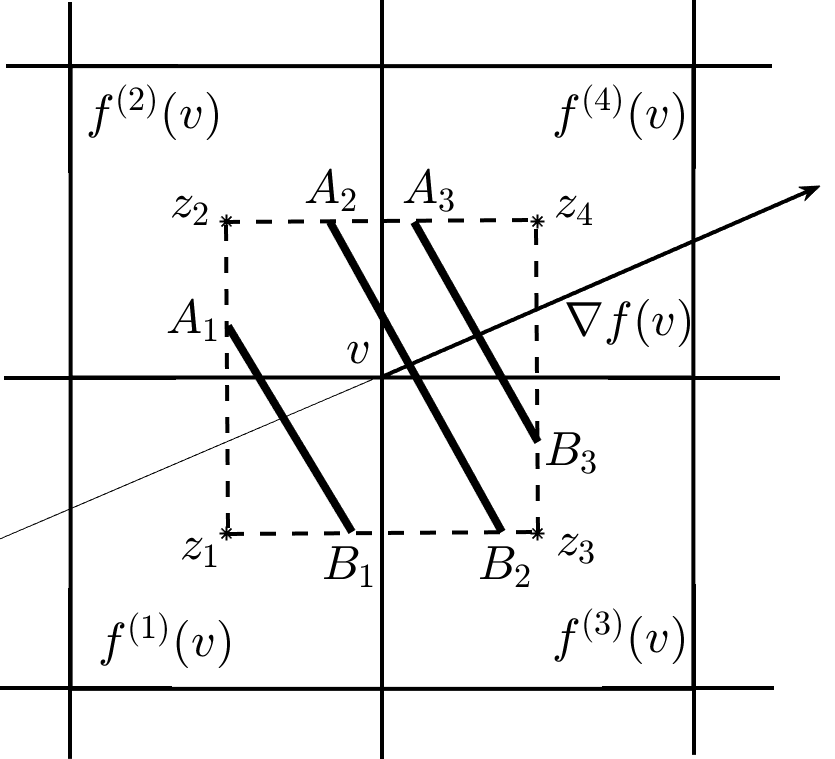
\includegraphics{FigLuPSquare2.png}
\end{center}
\caption{In each dual square, we compute the length of the segment that is the linear approximation of the level line $\{f=t\}$.}\label{UnbiasedPerim:fig}
\end{figure}


Define
\[
L_f^\eps(t,U) := \sum_{v\,\in\,\calV^{\Sq}_\eps\,\cap\,U} \sum_{j=1}^3
L_{j,\,f}^\eps(v,t) \ind_{f^{(j)}\,(v)\,<\,t\,\leq\, f^{(j+1)}(v)}.
\]
The following proposition shows that this way of computing the perimeter is unbiased.

\begin{prop}\label{unbiased-perim:prop}

Let $f$ be a $C^2$ function defined on $U^{\eps_0}$, for some $\eps_0>0$, such that $\min (|\partial_1 f(x)|, |\partial_2 f(x)|)<\max (|\partial_1 f(x)|, |\partial_2 f(x)|)$ for all $x\in U^{\eps_0}$. For $h\in C_b(\R)$, let us define the level unbiased perimeter integral as
\[
\LuP_f^\eps(h,U) := \int_\R h(f(t)) L_f^\eps(t,U) \, dt.
\]
Then $\LuP_f^\eps(h,U)$ converges to $\LP_f(h,U)$ as $\eps$ goes to $0$.
\end{prop}

\begin{proof}
By the coarea formula, since $f$ is $C^2$, we have
\[
\LP_f(h,U) = \int_\R h(t) \Per\left(E_f(t),U\right) \, dt = \int_U h(f(x))
\left\| \nabla f(x) \right\| \, dx.
\]
Using the definition of $\LuP_f^\eps(h,U)$, we can write
\begin{align*}
\LuP_f^\eps(h,U) &= \int h(f(t)) L_f^\eps(t,U) \, dt\\
&=\sum_{v\,\in\,\calV^{\Sq}_\eps\,\cap\,U}\; \sum_{j=1}^3 \int h(t)
L_{j,\,f}^\eps(v,t) \ind_{f^{(j)}\,(v)\,<\,t\,\leq\,f^{(j+1)}\,(v)} \, dt.
\end{align*}
The four values $f^{(k)}(v)$, $k=1,2,3,4$ are given by $\{ f(v +
\eps\tfrac{\sqrt{2}}{2}e_{\alpha_k})\}$ where the $e_{\alpha_k}$ are the unit vectors $\pm \frac{\sqrt{2}}{2} e_0 \pm \frac{\sqrt{2}}{2} e_{\frac{\pi}{2}}$. Therefore, using a first order Taylor expansion and denoting $\delta_1(v):=\min (|\partial_1 f(v)|, |\partial_2 f(v)|)$, resp. $\delta_2(v):=\max(|\partial_1 f(v)|, |\partial_2 f(v)|)$, since we assume $\delta_1(v)<\delta_2(v)$, we can write
\begin{align*}
f^{(1)}(v) &= f(v) - \eps \frac{1}{2}\left(\delta_1(v) + \delta_2(v)\right) + r_1(v,\eps),\\
f^{(2)}(v) &= f(v) + \eps \frac{1}{2}\left(\delta_1(v) - \delta_2(v)\right) + r_2(v,\eps) ,\\
f^{(3)}(v) &= f(v) - \eps \frac{1}{2}\left(\delta_1(v) - \delta_2(v)\right) + r_3(v,\eps),\\
f^{(4)}(v) &= f(v) + \eps \frac{1}{2}\left(\delta_1(v) + \delta_2(v)\right) + r_4(v,\eps),
\end{align*}
where $|r_k(v,\eps)|\leq \eps^2 \|D^2f\|$ for all $k$, with $\|D^2f\|:= \Sup_{x\in U} \| D^2f(x)\| < +\infty $. Then, we have
\[
\int_\R h(t)
L_{1,\,f}^\eps(v,t) \ind_{f^{(1)}\,(v)\,\leq\,t\,\leq\,f^{(2)}\,(v)} \, dt = h(f(v)) + \frac{\eps^2}{2} \frac{\delta_1(v)}{\delta_2(v)}
\sqrt{\delta_1(v)^2 + \delta_2(v)^2 } + \tilde{r_1}(v,\eps),
\]
where
$|\tilde{r_1}(v,\eps)|\leq C_{f,\,h,\,U} \eps^3$, with $C_{f,\,h,\,U}$ a constant that depends on $f$, $h$ and $U$ but not on $\eps$. In the following such a constant will be simply denoted $C$.

To compute the second integral, we first notice that $\forall t\in[f^{(2)}(v),f^{(3)}(v)]$, we have
\[
L_{2,\,f}^\eps(v,t)=
\frac{\eps}{\delta_2(v)} \sqrt{\delta_1(v)^2 + \delta_2(v)^2 } +
r'_2(v,\eps),
\]
with $|r'_2(v,t,\eps)|\leq C\eps^2$. Therefore we
obtain
\begin{multline*}
\int_\R h(t)
L_{2,\,f}^\eps(v,t) \ind_{f^{(2)}\,(v)\,\leq\,t\,\leq\,f^{(3)}\,(v)} \, dt \\
= h(f(v)) + \eps^2 \left(1-\frac{\delta_1(v)}{\delta_2(v)}\right)
\sqrt{\delta_1(v)^2 + \delta_2(v)^2 } + \tilde{r_2}(v,\eps),
\end{multline*}
where
$|\tilde{r_2}(v,\eps)|\leq C \eps^3$.

The third integral is computed in a way analogous to the first one, and we get the same approximation, namely
\[
\int_\R h(t)
L_{3,\,f}^\eps(v,t) \ind_{f^{(3)}\,(v)\,\leq\,t\,\leq\,f^{(4)}\,(v)} \, dt = h(f(v)) + \frac{\eps^2}{2} \frac{\delta_1(v)}{\delta_2(v)}
\sqrt{\delta_1(v)^2 + \delta_2(v)^2} + \tilde{r_3}(v,\eps),
\]
where
$|\tilde{r_3}(v,\eps)|\leq C_{f,\,h,\,U} \eps^3$.

Summing these three estimates and noticing that $\sqrt{\delta_1(v)^2 +
\delta_2(v)^2} = \| \nabla f(v) \| $, we obtain
\[
\LuP_f^\eps(h,U) = \sum_{v\,\in\,\calV^{\Sq}_\eps\,\cap\,U} \eps^2 h(f(v)) \left\| \nabla f(v)\right\|
+ \tilde{r}(\eps),
\]
that converges to $ \LP_f(h,U)$ as $\eps$ goes to $0$ thanks to Proposition~\ref{approx:prop}.
\end{proof}
%\vspace{5em}

\newpage
\bibliography{AHL_Bierme}
\end{document}
